%%%%%%%%%%%%%%%%%%%%%%%%%%%%%%%%%
%% usmthesis.cls 2016/12/08 version V1.7.
%%
%% IMPORTANT MESSAGE (Dec 2016)
%% Due to the recent numerous changes requested by IPS, USM to different
%% candidates -- often conflicting even within the same week -- without much
%% consistency nor in black in white, I have found it increasingly difficult
%% to maintain a coherent version. I have therefore decided to provide some
%% options that seem to be favored by IPS on different occasions; but will no
%% longer update the template until an updated formatting guidelines with clear
%% instructions and concrete samples is published.
%%
%% THERE WILL BE NO FURTHER UPDATES UNTIL IPS-USM PUBLISHES AN OFFICIAL
%% UPDATED FORMATTING GUIDELINES WITH CONCRETE, CLEAR INSTRUCTIONS.
%%
%% Individual requests for help to modify this version for your needs will be
%% handled on a case by case basis, depending on my mood, perhaps for a fee.
%% Requests for help to modify past versions will NOT be entertained.
%% Please read http://tex.my/how-to-ask-for-latex-related-help-effectively/.
%%
%% (Yes I'm that tired and frustrated. I know everyone just want to graduate,
%% but I am by now genuinely put off by the tone of some requests with rude
%% attitudes, unclear descriptions, flip-flopping conditions, etc for something
%% that was originally for my own use.)
%%
%% Usmthesis _was_ fun; but it has ceased to be so for me.
%%
%% Submit a git pull request on https://github.com/liantze/usmthesis
%% if you wish to contribute your changes. No timeframe is set for approvals.
%% I cannot check through any edited usmthesis.cls of any version without
%% CVS.
%%
%% Oh and if you'd like to adapt this template (the .cls and/or the .tex) for
%% your institution, that's perfectly fine, but at least keep the license
%% (LPPL 1.3) and the original author (me) won't you? It's just normal decency.
%% THANK you. :-)
%%%%%%%%%%%%%%%%%%%%%%%%%%%%%%%%%

%% If you prefer -- and have been allowed -- to use
%% Arial, then
%% \documentclass[arial]{usmthesis}
%% It's not really Arial, it's a Helvetica look-alike,
%% but if you're not a designer nor a typographer, you
%% probably can't tell the difference (I can't either)
%%
%% OTHER IMPORTANT OPTIONS:
%% singespacetitle - Make title on cover and title
%%                   page single-spaced.
%%
%% chapnumwords — Make chapter titles be `Chapter One'
%% tocchapnumwords — Make the ToC use `Chaper One' too
%%   (Engineering IPS seems to like the above two settings)
%%
%% tocpage   These options will add a ``Page'' label at the
%% lotpage   top of the Table of Contents, List of Tables,
%% lofpage   List of Figures and List of Plates respectively.
%% loppage   I don't know lah, one moment IPS says must add at
%%           the top of all these lists; one month later say
%%           only the ToC, a few months later say don't add at all.
%%           Find, mix-and-match yourself based on the instrustions you got.
%%
%% tocCAPSfront - Sometimes IPS wants the ``Table of Contents'', ``List of
%%                Figures'', ``Abstract'' etc to be all-caps in the ToC;
%%                sometimes they don't. Use this option to make them ALL CAPS.
%%
%% tocCAPSref - Similar to the above but for the ``References''.
%% tocCAPSapp - Similar to the above but for the ``Appendices''.
\documentclass[
singlespacetitle, % Make title on cover page singlespaced
% chapnumwords,tocchapnumwords,  %% ``Chapter One'' I think Engineering like this
tocpage,  % Put ``Page'' at top of ToC. Add lotpage, lofpage if
          % ``Page'' is also needed for LoT and LoF.
% tocCAPSfront, % Make ``List of Tables'' etc in ToC CAPS
% tocCAPSref, % Make ``References'' in ToC CAPS
% tocCAPSapp, % Make ``Appendices'' in ToC CAPS
]{usmthesis}

%%%%%%%%%%%%%%%%%%%%%%%%%%%%%%%%%%%%%%%%%%%%%%%%%%%%%%%
% This is usmthesis.tex, 6 Dec 2016. READ THE COMMENTS.
% Some formattings are easiest changed by uncommenting
% some lines in this .tex file or by changing certain
% options.
%
% Created by Lim Lian Tze (Ph.D.)
% liantze@gmail.com
% http://liantze.penguinattack.org.
%%%%%%%%%%%%%%%%%%%%%%%%%%%%%%%%%%%%%%%%%%%%%%%%%%%%%%%

\usepackage{pdfpages}
\usepackage{afterpage}
\usepackage{import}

% Set font size to 13pt
\usepackage{scrextend}
\changefontsizes{13pt}
\usepackage{pdflscape}

%% Example of loading other packages that you may require.
%% I'm loading the marvosym package so that I can produce a
%% smiley face with the command \Smiley.
\usepackage{marvosym}
\usepackage[inkscapelatex=false]{svg}

%% Also, the enumitem package is great for customising
%% list environments.
\usepackage{enumitem}
\usepackage{tabu}
\usepackage{booktabs}
\usepackage{calligra}
\usepackage{multirow}
\usepackage{multicol}
\usepackage{bm}
\usepackage{bibentry}
\usepackage{booktabs,caption}
\usepackage[flushleft]{threeparttable}
% \usepackage[capposition=top]{floatrow}
\usepackage{breakurl}

%% Listings is a nice package for typesetting code
%% listings. Other possible packages include fancyvrb,
%% minted, etc.
% \usepackage{listings}
% \lstset{basicstyle=\ttfamily,breaklines=true}

%% For those who need to produce algorithms and pseudocode.
%% There are a number of different packages available, but
%% unfortunately they tend not to work well together!
%% I'm using algorithmicx, specifically algpseucode, here.
\usepackage{algpseudocode}
\usepackage{algorithm}
\usepackage{indentfirst}
\usepackage{multirow}
\usepackage{dutchcal}
\usepackage{changepage}

\usepackage{xcolor}
\usepackage{amsfonts}
\colorlet{punct}{red!60!black}
\definecolor{background}{HTML}{EEEEEE}
\definecolor{delim}{RGB}{20,105,176}
\colorlet{numb}{magenta!60!black}
\usepackage{listings}
\lstdefinelanguage{json}{
    basicstyle=\normalfont\ttfamily,
    numbers=left,
    numberstyle=\scriptsize,
    stepnumber=1,
    numbersep=8pt,
    showstringspaces=false,
    breaklines=true,
    frame=lines,
    backgroundcolor=\color{background},
    literate=
     *{0}{{{\color{numb}0}}}{1}
      {1}{{{\color{numb}1}}}{1}
      {2}{{{\color{numb}2}}}{1}
      {3}{{{\color{numb}3}}}{1}
      {4}{{{\color{numb}4}}}{1}
      {5}{{{\color{numb}5}}}{1}
      {6}{{{\color{numb}6}}}{1}
      {7}{{{\color{numb}7}}}{1}
      {8}{{{\color{numb}8}}}{1}
      {9}{{{\color{numb}9}}}{1}
      {:}{{{\color{punct}{:}}}}{1}
      {,}{{{\color{punct}{,}}}}{1}
      {\{}{{{\color{delim}{\{}}}}{1}
      {\}}{{{\color{delim}{\}}}}}{1}
      {[}{{{\color{delim}{[}}}}{1}
      {]}{{{\color{delim}{]}}}}{1},
}
\lstset{
    numbers=left,
    breaklines=true,
    backgroundcolor=\color{light-gray},
    tabsize=2,
    basicstyle=\ttfamily,
    literate={\ \ }{{\ }}1
}
\lstdefinelanguage{SQL}{
    morekeywords={
        SELECT, INSERT, UPDATE, DELETE, FROM, WHERE, AND, OR, NOT, NULL, IS, 
        CREATE, ALTER, DROP, TABLE, DATABASE, INDEX, VIEW, TRIGGER, PROCEDURE, 
        FUNCTION, RETURNS, BEGIN, END, AS, DECLARE, SET, IF, ELSE, CASE, 
        WHEN, THEN, LOOP, FOR, WHILE, DO, RETURN, PRIMARY, FOREIGN, KEY, 
        REFERENCES, JOIN, INNER, LEFT, RIGHT, FULL, OUTER, ON, GROUP, BY, 
        ORDER, HAVING, DISTINCT, UNION, ALL, INTO, VALUES, LIMIT, OFFSET, 
        GRANT, REVOKE, COMMIT, ROLLBACK, TRANSACTION, EXPLAIN, ANALYZE
    },
    sensitive=false,
    morecomment=[l]{--},
    morecomment=[s]{/*}{*/},
    morestring=[b]',
    morestring=[b]",
    keywordstyle=\color{blue}\bfseries,
    commentstyle=\color{gray}\ttfamily,
    stringstyle=\color{orange},
    identifierstyle=\color{black},
    basicstyle=\ttfamily\footnotesize,
    breaklines=true,
    breakatwhitespace=true,
    showstringspaces=false
}


\usepackage{caption}

\usepackage{varwidth}
\DeclareCaptionFormat{myformat}{%
  % #1: label (e.g. "Table 1")
  % #2: separator (e.g. ": ")
  % #3: caption text
  \begin{varwidth}{\linewidth}%
    \centering
    #1#2#3%
  \end{varwidth}%
}

%% PHAT PLACE
\usepackage{caption}
\usepackage{graphicx}
%% NHAT PLACE
\usepackage{amssymb}% http://ctan.org/pkg/amssymb
\usepackage{pifont}% http://ctan.org/pkg/pifont
\newcommand{\cmark}{\ding{51}}%
\newcommand{\xmark}{\ding{55}}%
% \usepackage{subcaption} ERROR ?
\usepackage{ulem}
\newcommand{\tvhung}[2]{\sout{#1}\textcolor{blue}{\textbf{#2}}}
%------------------------------

%% Enter particulars about your thesis HERE
% Your Name
\author{LE LONG TRUONG THINH \hspace{5mm} 21125079 \\ HOANG THE TRUNG \hspace{5mm} 21120583}

% English title of your thesis
\title{ANNOTATION SYSTEM FOR MEDICAL DATA WITH SMART ASSISTANCE}
% Vietnamese title of your thesis
% \title{Phát triển giải pháp hỗ trợ y tế thông minh với các thuật toán học sâu trên dữ liệu thị giác}
% Malay title of your thesis
% \titlems{Penulisan Tesis dengan LaTeX}
% Year submitted
\submityear{2025}
% Month submitted
\submitmonth{March}
%% Choose only 1 degree type! :-)
\degreetype{BACHELOR OF SCIENCE IN COMPUTER SCIENCE}
% \degreetype{Master of Science}
\lecturer{ASSOC. PROF. TRẦN MINH TRIẾT \\ M.Sc. Đỗ Trọng Lễ}
% \lecturer{MSC. ĐỖ TRỌNG LỄ}

%%%%%%%%%%%%%%%%%%%%%%%%%%%%%%%%%%%%%%%%%%%%%%%%%%%%%%%
% You can comment out the following line if you don't have a
% "List of Own Publications". And make it all caps yourself
% if it needs to be all caps in the ToC.
%%%%%%%%%%%%%%%%%%%%%%%%%%%%%%%%%%%%%%%%%%%%%%%%%%%%%%%
\newcites{own}{List of Publications}
\newcites{ownnew}{List of Directed Publications}

\usepackage[plainpages=false,bookmarksnumbered,
bookmarksdepth=section,breaklinks=true]{hyperref}
%%%%%%%%%%%%%%%%%%%%%%%%%%%%%%%%%%%%%%%%%%%%%%%%%%%%%%%
% Options for generating hyperlinks when using pdfLaTeX
%%%%%%%%%%%%%%%%%%%%%%%%%%%%%%%%%%%%%%%%%%%%%%%%%%%%%%%

\hypersetup{
    colorlinks,
    citecolor=black,
    filecolor=black,
    linkcolor=black,
    urlcolor=black
}

\ifpdf
  \makeatletter
  \hypersetup{hypertexnames=false,%
    pdfauthor={\@author},pdftitle={\@title}}
  \makeatother
\fi

\usepackage{ragged2e}
\usepackage{tikz}
\usepackage{multido}
\usetikzlibrary{calc}
\usepackage{longtable}
\usepackage{makecell}
% https://tex.stackexchange.com/questions/64839/how-to-change-listing-caption
\renewcommand{\lstlistingname}{Block}
\usepackage{url}
% \def\UrlBreaks{\do\/\do-}
\usepackage{breakurl}

% \usepackage{pdflscape}

% \usepackage{amsmath}
% \DeclareMathOperator*{\argmax}{arg\,max}
% \DeclareMathOperator*{\argmin}{arg\,min}

\usepackage{listings}
\usepackage{xcolor}
\definecolor{light-gray}{gray}{0.9}
\lstdefinestyle{cSharp}{
    language=[Sharp]C,
    basicstyle=\ttfamily\scriptsize,
    numbers=left,
    numberstyle=\tiny\color{gray},
    stepnumber=1,
    numbersep=10pt,
    backgroundcolor=\color{white},
    showspaces=false,
    showstringspaces=false,
    showtabs=false,
    frame=single,
    breaklines=true,
    breakatwhitespace=false,
    tabsize=4,
    captionpos=b,
}

\lstset{
  language=JavaScript,
  basicstyle=\ttfamily\small,
  backgroundcolor=\color{gray!10},
  frame=single,
  breaklines=true,
  showstringspaces=false,
  keywordstyle=\color{blue}\bfseries,
  commentstyle=\color{gray}\itshape,
  stringstyle=\color{orange}
}


\setcounter{secnumdepth}{5}
\setcounter{tocdepth}{5}

\makeatletter
\newcommand\subsubsubsection{\@startsection{paragraph}{4}{\z@}{-2.5ex\@plus -1ex \@minus -.25ex}{1.25ex \@plus .25ex}{\normalfont\normalsize\bfseries}}
\newcommand\subsubsubsubsection{\@startsection{subparagraph}{5}{\z@}{-2.5ex\@plus -1ex \@minus -.25ex}{1.25ex \@plus .25ex}{\normalfont\normalsize\bfseries}}
\makeatother
\begin{document}

%%%%%%%%%%%%%%%%%%%%%%%%%%%%%%%%%%%%%%%%%%%%%%%%%%%%%%%
% Default bibliography style is apa (using
% \RequirePackage[natbibapa]{apacite} in the class file).
%
% If you prefer the number system though, use bibliography
% style "plainnat" for [1][2][3] or "alpha" for [Jon94] (the label
% will be auto-generated).
%%%%%%%%%%%%%%%%%%%%%%%%%%%%%%%%%%%%%%%%%%%%%%%%%%%%%%%
% \bibliographystyle{apacite}
% \bibliographystyleown{apacite}
% \bibliographystyle{plainnat}
% \bibliographystyleown{plainnat}
\bibliographystyle{ieeetr}
\bibliographystyleown{ieeetr}

%%%%%%%%%%%%%%%%%%%%%%%%%%%%%%%%%%%%%%%%%%%%%%%%%%%%%%%
% Inserts the cover page (the hard cover with gold-lettering)
% and the title page
%%%%%%%%%%%%%%%%%%%%%%%%%%%%%%%%%%%%%%%%%%%%%%%%%%%%%%%
\makecover
\frontmatter


%%%%%%%%%%%%%%%%%%%%%%%%%%%%%%%%%%%%%%%%%%%%%%%%%%%%%%%
% MAKE SURE YOU HAVE A acknowledgements.tex FILE
%%%%%%%%%%%%%%%%%%%%%%%%%%%%%%%%%%%%%%%%%%%%%%%%%%%%%%%

% \import{content/appendices}{advisor-comment.tex}
% \import{content/appendices}{reviewer-comment.tex}
% \includepdf[pages=-]{content/appendices/advisor_comment}
% \includepdf[pages=-]{content/appendices/reviewer_comment}
% \addtocounter{page}{-4}   
\import{content/appendices}{acknowledgements.tex}
% \import{content}{syllabus.tex}
% by FIT's requirement, proposal does not have page numbering
% and the page after the proposal (ToC) starts from ii
% 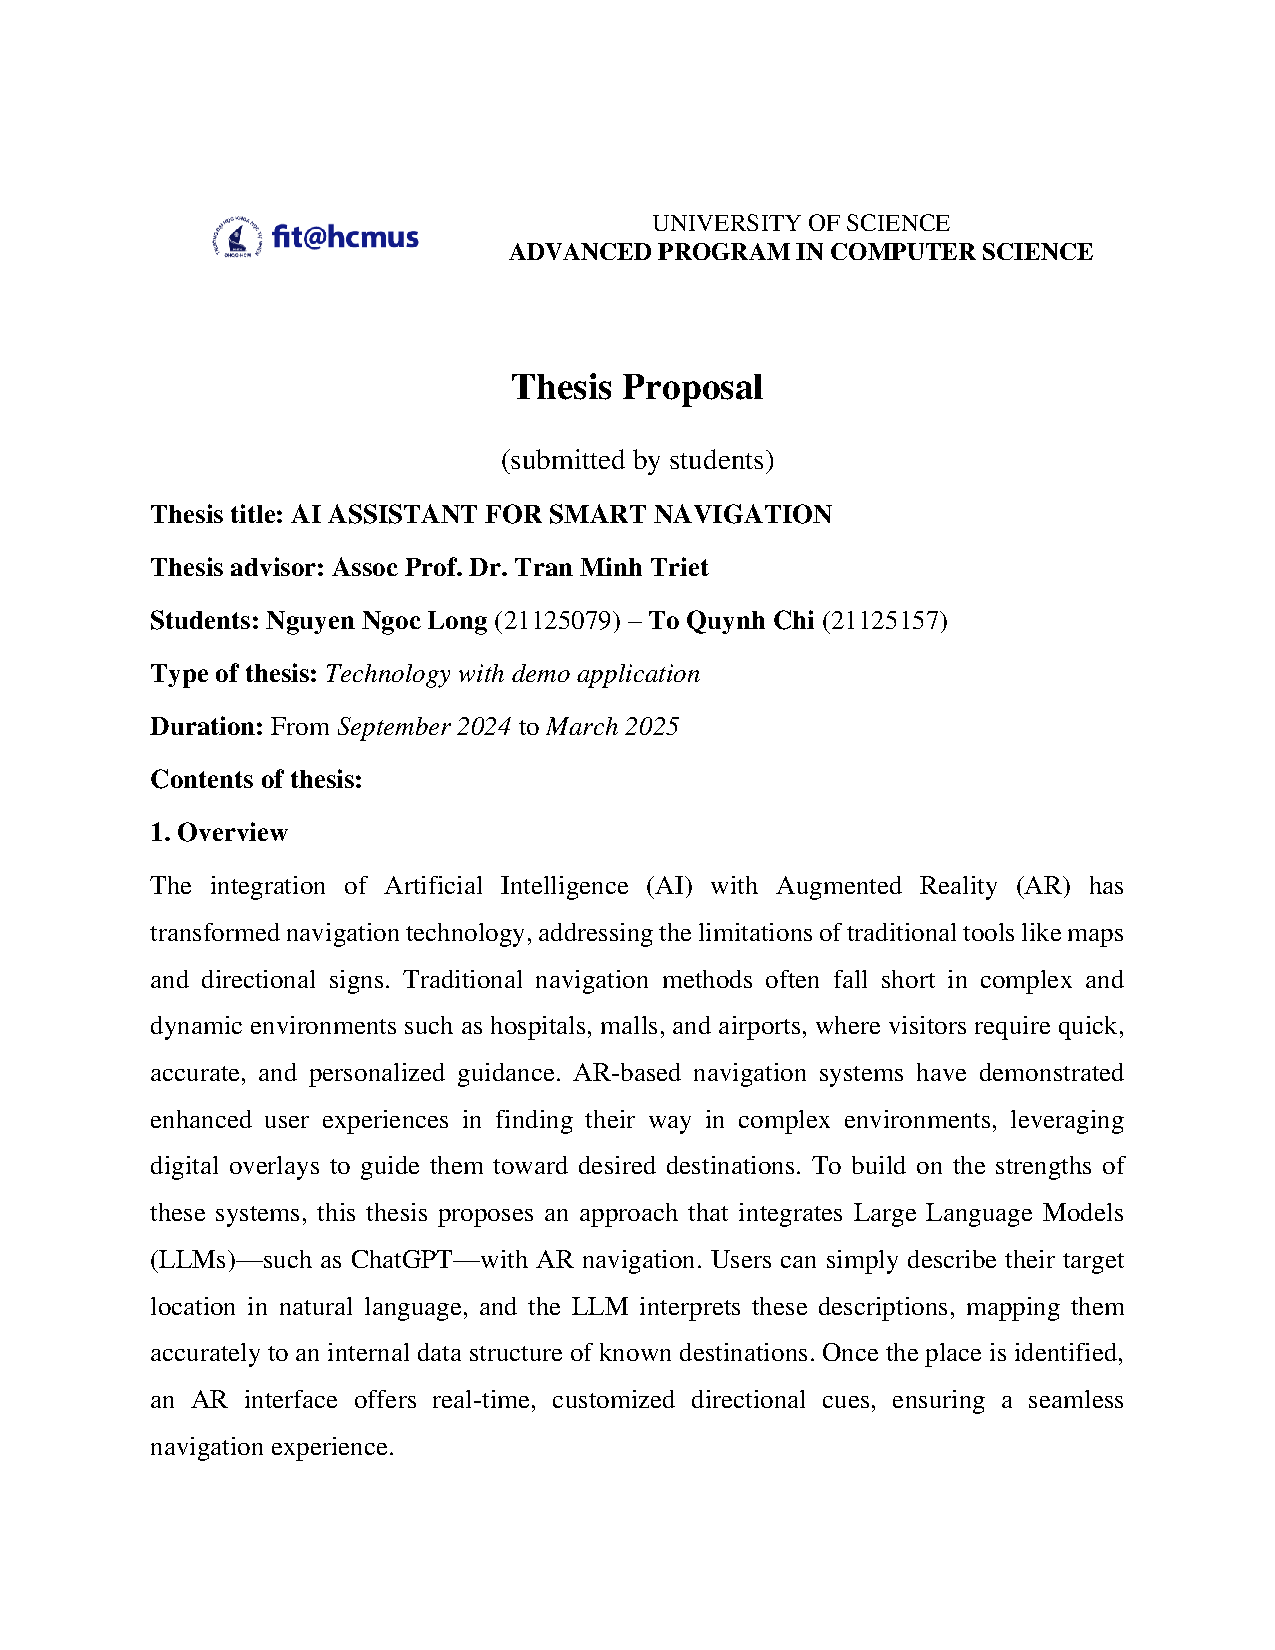
\includepdf[pages=-]{content/appendices/ThesisProposalOfficial}
\addtocounter{page}{-6}   
\tableofcontents \clearpage
%\listoftables \clearpage
%\listoffigures \clearpage
%%%%%%%%%%%%%%%%%%%%%%%%%%%%%%%%%%%%%%%%%%%%%%%%%%%%%%%
% You can comment out the following line if you don't
% have a "List of Plates"
%%%%%%%%%%%%%%%%%%%%%%%%%%%%%%%%%%%%%%%%%%%%%%%%%%%%%%%
% \listofplates \clearpage

%%%%%%%%%%%%%%%%%%%%%%%%%%%%%%%%%%%%%%%%%%%%%%%%%%%%%%%
% You can comment out the following line if you don't
% have a "List of Acronyms"
%%%%%%%%%%%%%%%%%%%%%%%%%%%%%%%%%%%%%%%%%%%%%%%%%%%%%%%
% \include{loa}

% Paragraph spacing
% \setlength\parskip{0.6em}
% Text-float spacing
\setlength\intextsep{24pt}

%%%%%%%%%%%%%%%%%%%%%%%%%%%%%%%%%%%%%%%%%%%%%%%%%%%%%%%
% Your Malay and English abstracts, each in one file.
%%%%%%%%%%%%%%%%%%%%%%%%%%%%%%%%%%%%%%%%%%%%%%%%%%%%%%%
% \input{abs-mal}
\begin{EnAbstract}
Medical imaging annotation remains a critical bottleneck in healthcare AI development, requiring extensive manual effort from medical experts and limiting the scalability of AI applications in clinical settings. This thesis presents the design, implementation, and evaluation of an intelligent medical annotation system that integrates AI assistance with clinical workflows to address these challenges.

The proposed solution consists of a four-component microservices architecture: (1) a React-based workflow management platform using Supabase for real-time collaboration and task orchestration; (2) an AI-enhanced annotation interface built on OHIF Viewer 3.x with integrated AI assistance capabilities; (3) a MONAI Label-based AI engine providing foundation model support including VISTA3D for multi-organ segmentation; and (4) an Orthanc PACS system for DICOM-compliant medical data management. This integrated approach enables seamless coordination between AI capabilities and medical expertise while maintaining compatibility with existing healthcare infrastructure.

The system implements novel AI-human collaboration mechanisms including interactive segmentation refinement, uncertainty visualization, and adaptive learning based on user corrections. A sophisticated workflow orchestration engine supports various annotation paradigms from simple single-annotator tasks to complex multi-stage collaborative workflows with quality control and consensus building.

The system design enables seamless integration with existing PACS infrastructure through standard DICOM protocols and provides a scalable foundation for AI-assisted medical annotation in healthcare environments. The platform demonstrates the feasibility of combining multiple specialized medical imaging tools into a unified, user-friendly interface that can adapt to various institutional requirements and clinical workflows.

The key contributions include a novel microservices integration architecture for medical imaging tools, an innovative AI-human collaboration framework optimized for medical annotation workflows, and a practical implementation that demonstrates the viability of AI-assisted annotation in clinical settings. This work provides a foundation for scalable medical annotation systems and contributes to advancing healthcare AI adoption in resource-constrained environments.

\end{EnAbstract}

\mainmatter

%%%%%%%%%%%%%%%%%%%%%%%%%%%%%%%%%%%%%%%%%%%%%%%%%%%%%%%
% The actual chapters of your thesis as listed in
% mainchaps.tex. Make sure you have the relevant
% chapter files.
% E.g. if you mainchaps.tex contains the lines
%
%  \include{hypothesis.tex}
%  \include{proof.tex}
%
% Then you MUST have the files hypothesis.tex, proof.tex
% (containing the relevant chapters) in the same directory
% as mainchaps.tex.
%%%%%%%%%%%%%%%%%%%%%%%%%%%%%%%%%%%%%%%%%%%%%%%%%%%%%%%
% 
\chapter{Introduction}
\label{sec:Introduction}
\label{Chapter1}

\begin{ChapAbstract}
Chapter 1 introduces the critical role of high-quality annotated data in modern machine learning and identifies the significant limitations of existing data annotation platforms, particularly their rigid workflows, insufficient auditability, and inflexible access control. It motivates the need for a novel platform designed to be flexible, auditable, and scalable, capable of supporting complex, real-world annotation pipelines. The chapter outlines the thesis objectives: to design and implement a platform with a dynamic, graph-based workflow engine, a fine-grained Attribute-Based Access Control (ABAC) system, and comprehensive audit trails. It highlights the benefits of these architectural components, emphasizing the platform's extensibility through its integration with specialized tools like OHIF Viewer, MONAI Label, and Orthanc for domains such as medical imaging. This introduction sets the stage for the detailed system design, implementation, and evaluation presented in the subsequent chapters.
\end{ChapAbstract}

\section{Overview}
\label{Chapter1-overview}

The rapid advancement of machine learning (ML) and artificial intelligence (AI) has led to the proliferation of sophisticated systems, from advanced analytical interfaces to large language models (LLMs), which are increasingly integral across diverse industries. The foundational efficacy of these systems is predicated upon the availability of high-quality, meticulously managed data. Within this paradigm, data annotation emerges as a critical process, transforming raw, unstructured information—such as images, text, audio, or video—into structured, labeled datasets that ML algorithms can effectively process and learn from. This precise labeling enables machines to interpret complex real-world phenomena, make accurate predictions, and execute decisions aligned with human perception and knowledge. 

The exponential growth in manuscript submissions to premier ML venues, including NeurIPS, ICML, and ICLR, underscores a profound and escalating demand not merely for increased data volume, but for data characterized by superior quality, enhanced granularity, and robust structural integrity. For instance, the development of AI systems aimed at augmenting scientific validation, such as those supporting factual verification or guiding reviewer performance, critically depends on access to "more granular, structured, and ethically-sourced peer review process data". This highlights that the pervasive need for high-quality, structured data extends beyond conventional model training, becoming a prerequisite for maintaining the integrity and scalability of scientific validation itself. Consequently, the success and ethical deployment of advanced AI are directly constrained by the current state of data annotation. Substandard data quality does not merely lead to minor technical inefficiencies; it results in systemic model failures, significant financial losses, and an erosion of trust in AI systems. Therefore, data annotation is not merely a preparatory technical step but a critical function for risk management and trust-building within the AI development lifecycle. 


\subsection*{Impact of Data Quality on Model Performance and Reliability}

A critical challenge in machine learning (ML) development is the tendency to prioritize data quantity over quality, which can significantly impair model performance and reliability. The use of low-quality data in training directly contributes to biased and inaccurate predictions, leading to suboptimal decision-making. The consequences of poor data quality are far-reaching, manifesting in several detrimental effects across the AI model lifecycle. These include diminished model accuracy, precision, and recall; biased predictions resulting in unfair or erroneous outcomes; and phenomena such as model hallucinations, where AI systems produce nonsensical or incorrect outputs. Additionally, poor data quality can precipitate model failures in production, incurring substantial financial costs, necessitating extensive data cleansing efforts, and eroding trust in AI initiatives. It also exacerbates technical debt and increases maintenance burdens due to inherent dataset flaws.

% Discussing common data quality issues
Common data quality issues in ML development include sparse data, characterized by incomplete or missing entries; noisy data, encompassing irrelevant, duplicate, or inaccurate information; and harmful data, which may embed biases against specific groups or include sensitive information vulnerable to training data poisoning. These challenges underscore the need for robust data quality strategies, such as comprehensive data cleansing, automated quality validation (e.g., schema validation, statistical checks, completeness assessments, and anomaly detection), and active learning techniques to enhance data reliability and volume.

% Highlighting the role of data annotation
The direct correlation between data quality and biased model predictions, coupled with the imperative for fairness and inclusivity in AI systems, positions data annotation as a cornerstone of responsible AI development. The design of annotation processes and platforms carries significant ethical and societal implications, extending beyond technical performance metrics. The growing emphasis on ``structured summaries'' and ``ethically-sourced peer review process data'' redefines ``high-quality data'' to encompass not only label accuracy but also the structural integrity and ethical provenance of datasets. This necessitates advanced annotation capabilities that transcend basic labeling, supporting complex, multi-layered data structuring and incorporating mechanisms for bias detection and mitigation at the source.

% Concluding the section
These considerations highlight the critical role of intelligent annotation assistance in addressing data quality challenges, ensuring robust, fair, and ethically sound AI systems capable of meeting the demands of modern applications.
\section{Motivation}
\label{sec:chapter-1-motivation}

Despite the critical importance of high-quality data annotation, existing platforms often exhibit significant shortcomings and inherent challenges. These limitations, particularly concerning rigid workflow designs, insufficient auditability, and inflexible access control mechanisms, prevent the efficiency, and reliability deployment of machine learning applications \cite{johnson2021challenges}. Addressing these deficiencies is paramount for supporting the intricate demands of complex, real-world ML annotation pipelines.

\subsection{Limitations of Existing Data Annotation Platforms}
Many contemporary data annotation platforms are characterized by rigid, predefined workflows that prove difficult to modify \cite{li2022annotation}. This inherent inflexibility leads to substantial inefficiencies, especially within the dynamic and iterative nature of modern AI projects. Specific issues include unclear or incomplete guidelines, which result in inconsistent and unreliable annotations \cite{chen2020guideline}, and a misalignment between annotators' tasks and the ultimate model goals, often leading to incorrect labeling. Furthermore, the use of inefficient annotation tools and poorly structured workflows slows down processes and increases the likelihood of errors \cite{wang2019workflow}. Disorganized projects frequently lead to delays and bottlenecks, while overloading annotators with high volumes of work contributes to fatigue and diminished accuracy.

A significant failing in current platforms is the absence of robust quality control and oversight mechanisms \cite{parker2022quality}. Without stringent quality checks, annotation errors often go unnoticed, culminating in flawed datasets and, consequently, unreliable AI models \cite{smith2020dataquality}. This includes the lack of a multi-step review process or automated checks, inconsistent labeling across different annotators, and missing audits. The challenge is further compounded by the impracticality of reviewing every single label for accuracy at scale.

Existing platforms also frequently suffer from inflexible access control mechanisms. A lack of granular access controls often permits unrestricted access, significantly increasing the risk of unauthorized changes and data leaks \cite{davies2023security}. Traditional role-based access control (RBAC) systems, which assign permissions based on predefined roles, are often static and struggle to adapt to the complex, dynamic environments characteristic of modern data annotation.

Moreover, scaling annotation efforts for large datasets and complex projects presents considerable challenges, placing significantly strain on both human teams and technological tools \cite{garcia2021scalability}. This includes difficulties in managing diverse data types and accurately interpreting complex patterns, as well as ensuring data accuracy and consistency across vast volumes of information. The recent rise of synthetic data and LLM data labeling has introduced new layers of complexity, particularly concerning consistency and bias management within the annotation process itself \cite{brown2023synthetic}. These factors, combined with the high costs associated with quality annotation, make balancing budget constraints with quality standards a tricky endeavor \cite{miller2024cost}.

To further elucidate the inherent limitations of current offerings, Table \ref{tab:platform_limitations} provides a comparative analysis of selected prominent data annotation platforms against key functionalities crucial for advanced annotation tasks. While some platforms excel in specific areas, none provide a comprehensive solution addressing all the identified challenges, particularly in the intersection of intelligent assistance, robust quality control, and adaptive security for complex tasks like referring expression and video object segmentation.

\begin{table}[htbp]
    \centering
    \caption{Comparative Analysis of Existing Data Annotation Platforms}
    \label{tab:platform_limitations}
    \renewcommand{\arraystretch}{1.4}
    \begin{tabularx}{\textwidth}{|>{\raggedright\arraybackslash}X
                                    |>{\raggedright\arraybackslash}X
                                    |>{\raggedright\arraybackslash}X
                                    |>{\raggedright\arraybackslash}X|}
        \hline
        \textbf{Feature / Platform}
            & \textbf{Label Studio}
            & \textbf{OHIF Viewer}
            & \textbf{Slicer 3D} \\
        \hline
        \textbf{Workflow Adaptability}
            & Configurable via JSON
            & Rigid (Viewing focus)
            & Rigid and specialized \\
        \hline
        \textbf{Granular Access Control}
            & Basic RBAC
            & Limited (Integrated with PACS)
            & Not applicable (local use) \\
        \hline
        \textbf{Interaction between users}
            & Yes
            & No
            & No \\
        \hline
        \textbf{Advanced QA \& Audit Trails}
            & Moderate (Custom setup)
            & Limited (Basic logging)
            & Limited (Research focus) \\
        \hline
        \textbf{AI-in-the-Loop / Active Learning}
            & Basic (External integration)
            & Limited (Pre-segmentation)
            & Limited (Plugin-based AI) \\
        \hline
        \textbf{Support for Complex/Dynamic Tasks}
            & Good (General)
            & Highly Specialized (Medical viewing)
            & Highly Specialized (3D medical analysis) \\
        \hline
        \textbf{Support for Medical Data (e.g., DICOM)}
            & Yes (Generic, requires conversion)
            & Excellent (Native DICOM)
            & Excellent (Native DICOM, NIfTI) \\
        \hline
    \end{tabularx}
\end{table}

The identified limitations reveal a fundamental lack of adaptability and robust governance as the underlying issue with many existing platforms. Rigid workflows directly contribute to inconsistencies and inefficiencies, which, when coupled with insufficient quality control, inevitably result in flawed datasets. These flawed datasets then lead to model failures and an erosion of trust, creating a detrimental cycle of wasted investment and poor AI outcomes. The inflexibility in access control further exacerbates security and compliance risks. The emergence of LLMs and synthetic data introduces a new dimension of complexity that current platforms are ill-equipped to handle. This is not merely about scaling traditional annotation, but about managing consistency and mitigating novel biases introduced by AI-assisted labeling processes themselves. This implies that a modern platform must be designed with "AI-in-the-loop" annotation and its unique challenges in mind. Furthermore, the consequences of using low-quality data extend beyond technical performance to include cascading financial impacts and technical debt. This transforms the motivation for a new platform from a purely academic or technical exercise into a strategic business imperative for organizations investing heavily in AI, underscoring the real-world value proposition of the proposed thesis.

\subsection{The Need for a Modern, Flexible, Auditable, and Scalable Platform}
The limitations mentioned above underscore the pressing need for a new generation of data annotation platforms. Such a platform must transcend the capabilities of existing solutions by being inherently flexible and adaptive, capable of handling complex, real-world annotation pipelines that involve dynamic and evolving requirements, moving beyond rigid, predefined sequences. It must also be fully auditable and transparent, providing robust mechanisms for quality control, error detection, and detailed tracking of all actions and state transitions to ensure data integrity and accountability. Crucially, the platform must be scalable, designed to efficiently accommodate growing data volumes and project complexities without compromising performance or accuracy. Finally, it must incorporate advanced security features with fine-grained access control, capable of limiting user views to granular data based on individual and contextual attributes, rather than relying solely on static roles.
\section{Objective}
\label{sec:chapter-1-objectives}

This thesis aims to address shortcomings in existing data annotation platforms by designing and implementing a system with enhanced flexibility, security, extensibility, and auditability. The specific objectives are meticulously crafted to contribute directly to a more efficienta and reliable data annotation process for machine learning.

\subsection*{Objective 1. To design and implement a data annotation platform with a dynamic, graph-based workflow engine.}
This objective seeks to overcome the inherent rigidity of current annotation workflows by introducing a dynamic, graph-based engine. Conceptualized as a Directed Acyclic Graph (DAG), this engine will facilitate the flexible definition and execution of complex, multi-stage annotation pipelines, adapting to evolving requirements in real-time. Such an approach offers unparalleled flexibility, scalability, and efficiency by streamlining processes, reducing bottlenecks, and enabling real-time adjustments to rules and conditions. A visual, low-code pipeline builder will democratize the creation and management of sophisticated data preparation strategies. Furthermore, the dynamic workflow engine will provide operational intelligence through real-time insights and analytics, enabling identification of bottlenecks and optimization of resource allocation. This directly contributes to the agility necessary for iterative AI development, accelerating the machine learning lifecycle by allowing rapid experimentation with diverse annotation strategies.

\subsection*{Objective 2. To develop a fine-grained, Attribute-Based Access Control (ABAC) system for secure and contextual permissions.}
This objective directly addresses the limitations of inflexible access control by implementing an Attribute-Based Access Control (ABAC) system. ABAC determines permissions based on a dynamic combination of user, resource, and environmental attributes (e.g., job role, data classification, access location). Access decisions are made in real-time by evaluating these attributes against predefined policies. The benefits of ABAC are substantial: it enhances security by enforcing granular, context-aware controls; aids in compliance with stringent regulations (e.g., GDPR, HIPAA, NIST 800-53); scales effortlessly in rapidly growing enterprises and cloud environments; and reduces administrative burden by centralizing permission management. By dynamically evaluating a rich set of attributes, ABAC enables proactive risk mitigation, ensuring that access is granted or denied based on the contextual risk of an access attempt. This represents a fundamental shift from static, identity-based security to a context-aware approach, crucial for handling sensitive data and enabling secure collaboration.

\subsection*{Objective 3. To ensure the platform is extensible for integration with external data sources and machine learning models}
This objective underscores the platform's architectural design for seamless integration with diverse external data sources and various machine learning models. Extensibility will be achieved through comprehensive APIs facilitating automated imports, task creation, and exports, alongside robust support for cloud storage solutions. Crucially, the platform will support Man-in-the-Loop (MITL), also known as Human-in-the-Loop (HITL), systems. This involves leveraging AI-assisted labeling (e.g., pre-annotation using models like SAM or Grounding DINO, active learning) for initial suggestions, combined with robust human validation for quality control, bias mitigation, and handling complex edge cases. For specialized domains, such as medical imaging, extensibility will be demonstrated through integration with established tools like the OHIF Viewer for visualization, MONAI Label for AI-assisted annotation tailored for medical images, and Orthanc as a PACS server for data management. This symbiotic relationship between AI and human expertise will lead to continuously improving data quality and model performance, while the extensive integration capabilities position the platform as an integral component within broader MLOps pipelines.

\subsection*{Objective 4. To create a reliable system with comprehensive audit trails for all actions and state transitions.}
This objective aims to ensure the platform's reliability, traceability, and accountability by implementing robust audit logging and audit trail functionalities. Audit logging systematically records all significant activities and changes, capturing detailed information about user actions and system events. Audit trails then connect these discrete events into a detailed, narrative-driven timeline, illustrating the lineage and transformation of data. The importance of comprehensive audit trails is multifaceted: they provide accountability and traceability by documenting who performed each action, when, and why; they are vital for demonstrating compliance with legal and regulatory frameworks (e.g., GDPR, HIPAA, FDA 21 CFR Part 11); they enable early detection of unauthorized access or suspicious activities; and they assist in debugging and root cause analysis. Furthermore, transparency into data sources and transformations, facilitated by audit trails, fosters increased trust among stakeholders, helps identify and mitigate biases in datasets, and enhances the interpretability and explainability of AI models by meticulously tracking data lineage.
\label{chap1:sec4-thesis-content}

\section{Thesis Contents}
This introductory chapter has laid the foundational groundwork for the thesis, establishing the critical context for data annotation, identifying the significant research gap stemming from limitations in existing platforms, and clearly articulating the proposed solution through specific objectives and its defined scope. The subsequent chapters will delve into the detailed design, implementation, and rigorous evaluation of the proposed web-based data annotation platform.

\subsection*{Chapter 2. Literature Review}
  This chapter will provide a comprehensive and critical review of existing academic and industry literature pertinent to data annotation platforms, advanced workflow management systems, modern access control mechanisms, and the principles of auditability in complex software systems. It will analyze current approaches, identify their strengths and weaknesses, and precisely delineate the specific gaps that this thesis aims to address.

\subsection*{Chapter 3. System Design and Architecture}
 This chapter will detail the architectural design of the proposed web-based data annotation platform. It will elaborate on the chosen architectural patterns, the interconnections between its backend, middleware, and frontend components, and the specific design principles underpinning the dynamic, graph-based workflow engine, the fine-grained Attribute-Based Access Control (ABAC) system, and the comprehensive audit trail mechanism.

\subsection*{Chapter 4. Annotation System For Medical Data With Smart Assistance}
 This chapter will describe the technical implementation of the platform. It will outline the specific technologies, programming languages, frameworks, and methodologies employed in developing each core component. Furthermore, it will provide insights into the practical challenges encountered during the development process and the innovative solutions adopted to overcome them.

\subsection*{Chapter 5. Evaluation and Results}
 This chapter will present the methodology used for evaluating the implemented platform, followed by a detailed presentation and analysis of the results. It will rigorously assess the platform's performance, flexibility, security, auditability, and scalability against the defined thesis objectives, utilizing relevant quantitative and qualitative metrics, as well as illustrative use cases.

\subsection*{Chapter 6. Conclusion and Future Work}
 This final chapter will synthesize the key findings and contributions of the thesis to the field of data annotation and machine learning infrastructure. It will also critically discuss the limitations of the current work and propose promising directions for future research and development, suggesting avenues for extending the platform's capabilities and applicability.


\include{content/chapters/chap-intelligent-navigation-and-destination-management}
\chapter{System Design and Architecture}
\label{sec:System Design and Architecture}
\begin{ChapAbstract}
Chapter 3 delineates the comprehensive system design and architectural framework of the medical imaging data annotation platform. It elaborates on the strategic technology stack choices, the intricate design of both frontend and backend components, and the robust deployment infrastructure, all meticulously engineered to address the unique demands of medical data privacy, scalability, and AI-driven workflows.
\end{ChapAbstract}

\section{Technology Stack and Design Rationale}
The selection of the technology stack is predicated on achieving a highly scalable, maintainable, and secure platform, particularly critical for handling sensitive medical imaging data. This section justifies the architectural philosophy and the specific technologies chosen for each layer of the system.

\subsection{Architectural Philosophy}
The platform adopts a decoupled, multi-tiered architecture comprising a PostgreSQL-centric backend and a modern React frontend. This architectural philosophy is a strategic choice to ensure robust scalability, enhanced maintainability, and clear separation of concerns. By decoupling the frontend (user interface) from the backend (business logic and data storage), each layer can be developed, deployed, and scaled independently, optimizing resource utilization and facilitating parallel development. The backend, centered around PostgreSQL, provides a reliable and extensible data foundation, while the React frontend offers a highly responsive and modular user experience. This modularity simplifies debugging, updates, and the integration of new features or technologies without extensive rework, thereby enhancing the system's long-term viability and adaptability.

The following diagram provides a high-level overview of the platform's architectural components and their interconnections, illustrating the decoupled nature of the system and the flow of data between the user, frontend, backend, and external medical imaging/AI services.

\begin{figure}
    \centering
    \includegraphics[width=1\linewidth]{content//resources//architecture.png}
    \caption{Overview of the platform's architecture}
    \label{fig:enter-label}
\end{figure}

\subsection{Frontend Rationale (React \& Refine.dev)}
The frontend is built with React, a leading JavaScript library renowned for its component-based architecture and declarative nature. React's component model promotes reusability, modularity, and maintainability, allowing complex UIs to be efficiently assembled from smaller, independent units. This facilitates parallel development and ensures a consistent design language across the application. React is a highly popular choice, running on 4.8\% of websites globally and being leveraged by approximately 41.6\% of professional developers according to a 2024 StackOverflow report. Its component architecture is reported to produce 60\% faster development times compared to monolithic architectures, and React-built sites can render 15-20\% faster than other JavaScript library-based websites. 

To accelerate development and provide enterprise-level features, the platform leverages Refine.dev. Refine is a headless frontend framework that streamlines the creation of data-intensive applications like admin panels and dashboards. It offers pre-built components and hooks for common enterprise functionalities, including CRUD (Create, Read, Update, Delete) operations, robust authentication flows, and flexible routing, significantly reducing boilerplate code and development time. Refine's backend-agnostic nature ensures compatibility with the chosen Supabase backend, providing 100\% control over the project without workflow constraints. Refine.dev is noted for its ability to significantly increase development speed, allowing data-heavy apps to be set up in a short amount of time, often less than a minute using its CLI. It boasts a community of 32K+ active developers and is used in 8K+ production projects. 

For a comprehensive and consistent user interface, Ant Design is integrated. Ant Design is a widely adopted UI library that provides a rich collection of high-quality, customizable, and accessibility-compliant React components. Its adherence to a unified design language ensures a cohesive look and feel across the application, improving team collaboration and reducing design-to-development discrepancies.

Finally, Vite is employed as the build tool and development server. Vite offers significantly faster development experiences due to its instant server start, lightning-fast Hot Module Replacement (HMR), and efficient production builds. It leverages native ES modules for on-demand file serving, eliminating the need for bundling during development, and performs optimized builds with Rollup for production, including code splitting and tree shaking for smaller bundle sizes and faster load times. 

\subsection{Backend Rationale (Supabase \& PostgreSQL)}
The backend is architected around Supabase, an open-source Backend-as-a-Service (BaaS) platform that provides a managed PostgreSQL database, authentication, real-time capabilities, and serverless functions. Supabase was chosen as a robust alternative to traditional backend development, simplifying much of the heavy lifting while offering the flexibility and transparency of open-source tools. 

At its core, Supabase utilizes PostgreSQL, a highly reliable, extensible, and performant relational database system. PostgreSQL is a dominant force in the relational database market, holding a 16.85\% share as of 2025, making it the second most used open-source database after MySQL. It is also recognized as the

most admired and desired database in recent surveys. This choice allows the platform to leverage the full power of SQL, including advanced queries, JSON support, and ACID compliance, ensuring strong data integrity and transactional consistency. In performance comparisons, PostgreSQL within Supabase demonstrates significant advantages for complex queries, with complex joins completing in 89ms compared to Firebase's 251ms, and aggregations in 103ms versus Firebase's 327ms. 

A key architectural strategy is the embedding of core business logic directly within PostgreSQL functions and triggers. This approach ensures atomicity and data integrity by executing logic directly at the database level, guaranteeing that operations are either fully completed or entirely rolled back. Triggers automatically execute SQL functions on table events (e.g., INSERT, UPDATE, DELETE), providing a powerful mechanism for enforcing business rules and maintaining data consistency directly within the database. While this approach can introduce challenges in debugging and potential vendor lock-in if overused , for critical business logic requiring high transactional integrity and direct data manipulation, it offers unparalleled reliability. 

\subsection{Medical Imaging \& AI Rationale (Orthanc, OHIF, MONAI)}
The selection of specialized tools for medical imaging and AI is crucial for addressing the domain-specific complexities and regulatory requirements.

\begin{itemize}
    \item \textbf{Orthanc}: Chosen as a lightweight, open-source DICOM server (mini-PACS). Orthanc simplifies the management and exchange of medical images by providing a modern RESTful API and full support for the DICOMweb standard (QIDO-RS, WADO-RS, STOW-RS). Its design abstracts the inherent complexity of the DICOM format and protocol, allowing developers to interact with medical images with minimal DICOM knowledge. This significantly reduces development overhead and accelerates the integration of medical imaging data into the web-based platform. Orthanc is noted for its lightweight nature and ability to run on standard desktop computers, making deployment almost immediate.
    \item \textbf{OHIF Viewer}: Selected as a powerful, open-source, web-based medical imaging viewer. OHIF is designed for rapid loading and visualization of large radiology studies, leveraging Cornerstone3D for efficient rendering and annotation. Its React-based, component-driven architecture and flexible plugin framework allow for seamless embedding and customization within the platform's frontend. OHIF's out-of-the-box compatibility with DICOMweb archives like Orthanc further streamlines data access. While a large study of 2500 instances (800MB) can take approximately 30 seconds to display in the viewport , OHIF is continuously optimized for performance, including GPU acceleration and multi-threading for quick image decoding.
    \item \textbf{MONAI}: Utilized as a standardized, open-source framework for medical AI. MONAI Label, a component of MONAI, provides intelligent image labeling and learning tools that enable AI-assisted annotation, active learning, and continuous model improvement specifically for medical images. Its support for state-of-the-art models and integration capabilities with viewers like OHIF make it an indispensable component for building powerful, integrated medical AI workflows. MONAI Label is reported to enable 50-80\% faster annotation time and 2x faster model convergence. The MONAI ecosystem has seen significant adoption, with over 3.5 million downloads and contributions from 220 individuals globally, and has been acknowledged in over 3,000 publications.
\end{itemize}

This integrated system—Orthanc for data management, OHIF for visualization and annotation, and MONAI for AI-driven assistance—forms a modular and powerful ecosystem tailored for medical imaging data annotation, ensuring compliance, efficiency, and advanced AI capabilities. 

\subsection{Infrastructure Rationale (Nginx, Azure, Cloudflare)}
The infrastructure design prioritizes security, performance, and ease of deployment.

\begin{itemize}
    \item \textbf{Nginx}: Employed as a reverse proxy to manage and secure traffic to all backend services. Nginx sits in front of the backend servers, distributing client requests, performing load balancing, and acting as an additional layer of defense against security attacks. It centralizes SSL/TLS termination, compresses data, and caches content, thereby offloading work from backend servers and improving overall performance and security. Its role simplifies network configuration and enhances the anonymity of backend services. Nginx has seen a significant rise in popularity, surpassing Apache in market share, reaching 34.1\% by November 2023 and 33.8\% of all websites whose web server is known as of July 2025.
    \item \textbf{Azure VM}: Chosen for hosting stateful backend services, specifically Orthanc and MONAI. Azure Virtual Machines provide the necessary computational resources, persistent storage, and network configurations required for these services, which often demand dedicated resources and specific environments for optimal performance and data residency. This ensures full control over sensitive medical data, allowing deployment within a secure, on-premise or private cloud infrastructure to meet stringent data privacy and compliance requirements (e.g., HIPAA, GDPR).
    \item \textbf{Cloudflare Pages}: Utilized for deploying the frontend application with integrated CI/CD capabilities. Cloudflare Pages is a JAMstack platform designed for static websites and dynamic frontends built with frameworks like React. It offers easy setup by integrating with GitHub/GitLab repositories, providing automatic deployments on code pushes, a global CDN for low-latency responses, and built-in SSL certificates. This choice ensures rapid deployment, global accessibility, and efficient content delivery for the user-facing application. Cloudflare's global network caches static content within 50ms of 95\% of all Internet users, and its CDN can provide a 1900ms (nearly 2 second) improvement in load time for static content by reducing the physical distance between the client and the data.
\end{itemize}


\section{Frontend Design}
The frontend is meticulously designed to provide an intuitive, efficient, and highly responsive user experience for managing projects, building workflows, and performing precise medical image annotation.
\subsection{Frontend Application Framework: React \& Refine.dev}
The frontend's foundation is built upon React, a widely adopted JavaScript library celebrated for its component-based architecture. This paradigm promotes the development of reusable, self-contained UI units, which significantly enhances modularity, maintainability, and scalability of the application. React's declarative nature simplifies UI development, allowing complex interfaces to be efficiently composed from smaller, independent components. 

Building upon this robust React foundation, the platform extensively leverages Refine.dev, a headless frontend framework specifically engineered to accelerate the development of data-intensive applications such as admin panels and dashboards.

\subsubsection*{Problem Refine.dev Solves}
Traditional frontend development for data-intensive applications often faces several challenges:
\begin{itemize}
    \item \textbf{Boilerplate Code}: Implementing common enterprise features like CRUD (Create, Read, Update, Delete) operations, authentication, routing, and state management typically involves writing a significant amount of repetitive boilerplate code, which slows down development and increases maintenance burden.
    \item \textbf{Compromise between Speed and Flexibility}: Developers often have to choose between low-code tools that offer rapid initial setup but lack long-term customizability and full-code approaches that provide flexibility but require extensive manual coding.
    \item \textbf{Complex State and API Management}: Handling API networking, complex state management, and robust authentication/authorization flows in data-heavy applications can be intricate and error-prone.
\end{itemize}

\subsubsection*{How Refine.dev Solves It (Philosophy \& Features)}
Refine's philosophy centers on providing a "sweet spot between low-code and full-code," offering comparable initial development speed to drag-and-drop tools while ensuring infinite scalability for long-term complexity. It addresses the aforementioned pain points through its core features:

\begin{itemize}
    \item \textbf{Headless Architecture \& Decoupled UI}: Refine is "headless," meaning it provides the underlying logic and functionality without imposing a specific UI framework or design system. This allows developers 100\% control over the user interface, enabling seamless integration with any UI kit (e.g., Ant Design) or custom design, without being constrained by Refine's features interfering with the UI structure. Each UI component is exposed directly, not wrapped in an encapsulation layer, providing maximum flexibility.
    \item \textbf{Boilerplate-Free Code \& No Configuration}: Refine aims to eliminate repetitive tasks and boilerplate code, making projects easier to understand and maintain. It boasts an easy setup, allowing projects to be started in less than a minute using its Command Line Interface (CLI) program, which contributes to faster development times.
    \item \textbf{Backend Agnostic}: A core tenet of Refine's philosophy is its compatibility with any custom backend, including GraphQL, REST APIs, and specific integrations like Supabase, Strapi, and Firebase. This backend agnosticism prevents vendor lock-in and provides developers with complete control over their project's backend choices and workflows.
    \item \textbf{Comprehensive Feature Set}: Refine offers a complete suite of features essential for data-driven applications, including routing, networking, authentication, state management (leveraging React Query for caching and data handling), and internationalization (i18n). Its router-agnostic design allows integration with popular routing solutions like React Router and Next.js, providing automatic parameter detection and redirections.
    \item \textbf{Native TypeScript Core}: Refine is built with a native TypeScript core, enhancing code quality, maintainability, and developer experience by providing static type checking.
    \item \textbf{Built-in Support \& Community}: Refine provides built-in support for various services and boasts a strong open-source community with 31.6K+ stars on GitHub, 8K+ projects in production, and 32K+ active developers. This vibrant ecosystem ensures ongoing development, support, and a wealth of shared knowledge.
\end{itemize}

\subsection{Visual Workflow Orchestrator}
The platform integrates XYFlow to create a sophisticated visual, graph-based interface for composing annotation pipelines. XYFlow is a powerful library for building interactive node-based editors, providing the core engine for managing node states, complex edge routing, and automatic layouts. This visual builder empowers users, particularly project managers and researchers, to intuitively design and modify complex, multi-stage annotation workflows using a drag-and-drop interface. Custom nodes are developed to represent specific medical-imaging workflow stages, such as "Data Ingestion (Orthanc)," "MITL Node," "Human Annotator Node" and "Human Review Node" These nodes abstract the underlying technical complexities, allowing users to focus on the logical flow of the annotation process. The visual representation aids in understanding data flow, identifying bottlenecks, and making real-time adjustments, thereby enhancing overall efficiency and adaptability.

\subsection{Integrated Medical Imaging Annotation Environment}
The primary annotation interface is built around the direct embedding of the OHIF Viewer within the platform's main React application, creating a unified and high-performance environment for medical image annotation.
\subsubsection*{OHIF Viewer v3: Philosophy, Architecture, and Evolution}
The OHIF Viewer is an open-source, web-based medical imaging platform designed to provide a core framework for building complex imaging applications with user-friendly interfaces. Its philosophy centers on being highly configurable and extensible, allowing it to load images from various sources (including DICOMweb) and render them in 2D, 3D, or restructured representations. The viewer aims to load large radiology studies as quickly as possible by retrieving metadata ahead of time and streaming pixel data as needed.Historically, medical imaging software often comprised desktop applications that were challenging to debug remotely and maintain by IT staff. The OHIF Viewer emerged in this context as an attractive web-based solution, leveraging cloud computing principles.
\subsubsection*{OHIF Viewer v2 Architecture and Challenges}
In its earlier iterations (e.g., v2), OHIF Viewer was built with React using reusable UI components, but its architecture presented challenges, particularly with extensions being hard to maintain. Creating new workflows often required building new UI components and extensions from scratch, which could be cumbersome. The direct embedding via a <script> tag, while possible, was deprecated in version 3, indicating a shift towards a more integrated and robust embedding strategy.
\subsubsection*{OHIF Viewer v3: Modernized Architecture and Solutions:}
OHIF Viewer v3 represents a significant re-architecture, transitioning to a modernized structure with TypeScript and ES module support. This transition enhances stability, accelerates development cycles, and improves accessibility. Key architectural components in v3 include:
\begin{itemize}
    \item \textbf{Core Libraries}: Implement medical imaging functions (business logic) for the web. UI Component Library (@ohif/ui-next): Built using shadcn/ui, providing a modern, compact layout for panels (e.g., Study Browser, Measurement, Segmentation) and offering enhanced theming and customization options.
    \item \textbf{Extensions}: Libraries implementing essential functionalities like rendering and measurement tracking. These are the building blocks consumed by modes.
    \item \textbf{Modes}: A pivotal new concept in v3. Modes are configuration objects that compose extensions and routes to create specific application workflows or "mini-apps" within a single viewer. This allows users to utilize common extensions with different configurations, significantly enhancing customizability and eliminating the need to duplicate viewer codebase for new workflows.
    \item \textbf{Cornerstone3D}: The underlying rendering and tooling library, providing a more robust and stable foundation for 3D rendering and annotations, and supporting features like GPU acceleration and multi-threading for quick image decoding.
    \item \textbf{Performance Optimizations}: V3 leverages React 18 for concurrent rendering, offers automatic preloading of the next series to reduce loading times, and integrates Web Worker Manager to offload intensive tasks without impacting UI performance.
\end{itemize}
This modular and extensible framework allows users to focus on their specific use cases without worrying about the underlying infrastructure, providing significant benefits for custom project adjustments. Users can customize the viewer for their specific workflows and add new functionalities without forking the entire codebase. This flexibility is crucial for researchers and developers who need to adapt the viewer to unique project requirements or integrate it with proprietary systems.
\subsubsection*{Integration with MONAI Label Interface for AI-Assisted Labeling}
The platform facilitates a seamless integration of the MONAI Label interface directly into the OHIF Viewer, enabling powerful AI-assisted annotation workflows. This integration is a result of a partnership between OHIF and NVIDIA to migrate the MONAI Label plugin to the OHIF Viewer v3 platform.
\subsubsection*{MONAI Label Integration and Interaction:}
This integration allows users to effortlessly connect their MONAI Label server to OHIF Viewer v3, leveraging a wide range of advanced AI features. MONAI Label, as an intelligent image labeling and learning tool, combines AI assistance with clinical expertise to deliver fast, accurate, and consistent annotations.The interaction flow is as follows:
\begin{itemize}
    \item \textbf{AI-Assisted Pre-labeling}: The MONAI Label server, connected to the OHIF Viewer, can generate initial segmentation masks or other predictions for medical images. This significantly accelerates the initial labeling process by providing real-time AI assistance, enabling 50-80\% faster annotation time.
    \item \textbf{Human Review and Refinement}: Human annotators review and refine these AI-generated labels directly within the OHIF Viewer's comprehensive suite of tools (e.g., brushes, erasers, shapes, and thresholding tools).
    \item \textbf{Active Learning and Continuous Improvement}: The system supports active learning mechanisms, where the MONAI model intelligently queries humans for annotations on uncertain or challenging examples, optimizing the annotation process. Human-corrected annotations from the OHIF Viewer are systematically fed back to the MONAI Label server for re-training or fine-tuning, ensuring that the AI models continuously learn from real-world user interactions and progressively enhance their performance over time, leading to 2x faster model convergence.
    \item \textbf{Data Flow}: OHIF Viewer can connect directly to a MONAI Label server, which in turn can connect to local or remote DICOM-web storage (like Orthanc) to access medical images. This seamless data flow enables the entire Human-in-the-Loop (HITL) process, where AI suggestions are presented, refined by humans, and then used to improve the AI models.
\end{itemize}

This tight integration of OHIF Viewer with MONAI Label provides a powerful environment for medical image annotation, combining high-performance visualization with cutting-edge AI capabilities to accelerate research and clinical AI development.
\section{Backend Design (Supabase \& PostgreSQL)}

This section details the backend architecture of the data annotation platform, which is built entirely on the Supabase platform, leveraging its integrated services to create a robust, scalable, and secure system.

\subsection{Supabase as the Backend Foundation}

The backend is architected around Supabase, an open-source Backend-as-a-Service (BaaS) platform that provides a managed PostgreSQL database, authentication, real-time capabilities, and serverless functions. Supabase was chosen as a robust alternative to traditional backend development, simplifying much of the heavy lifting while offering the flexibility and transparency of open-source tools.

Unlike proprietary BaaS solutions, Supabase is built with open-source tools, primarily PostgreSQL, providing developers with the full power of SQL while benefiting from a stable and scalable managed infrastructure.

\textbf{Core Components Utilized:}
\begin{itemize}
    \item \textbf{PostgreSQL Database:} At the heart of Supabase is PostgreSQL, a highly reliable, extensible, and performant relational database system. PostgreSQL is a dominant force in the relational database market, holding a 16.85\% share as of 2025, making it the second most used open-source database after MySQL. It is also recognized as the most admired and desired database in recent surveys. This choice allows the platform to leverage the full power of SQL, including advanced queries, JSON support, and ACID compliance, ensuring strong data integrity and transactional consistency. In performance comparisons, PostgreSQL within Supabase demonstrates significant advantages for complex queries, with complex joins completing in 89ms compared to Firebase's 251ms, and aggregations in 103ms versus Firebase's 327ms.
    \item \textbf{Supabase Auth:} This component provides secure user authentication and management, enabling features like user registration, login, session management, password resets, and email verification with minimal code. It supports various authentication methods, including email/password and social logins.
    \item \textbf{Supabase Realtime:} Leveraging PostgreSQL replication, Supabase's Realtime engine provides live data synchronization, allowing the frontend to react instantly to database changes. This is crucial for collaborative environments and real-time notifications.
\end{itemize}

\subsection{Database Schema and Data Model}

The database schema is meticulously designed to store platform-specific entities and efficiently manage DICOM metadata, adhering to principles of logical data separation and robust security.

\subsubsection*{Logical Data Separation:}
\begin{itemize}
    \item \textbf{Core Tables (\_ prefix):} Raw, normalized data tables (e.g., \_projects, \_tasks, \_users, \_annotations, \_workflows, \_studies, \_series, \_instances) are prefixed with an underscore. These tables are considered internal and are not directly exposed to the frontend. This convention protects data integrity by ensuring that direct modifications bypass the defined business logic and security policies.
    \item \textbf{Data Views:} The primary interface for the application is provided through secure views (e.g., \texttt{projects}, \texttt{tasks}). These views join and expose data from the core tables, acting as a secure and flexible API layer. This abstraction allows fine-grained control over what data is visible and how it can be accessed by different user roles, thereby enforcing the Attribute-Based Access Control (ABAC) model at the database level. This design ensures the platform can efficiently handle the unique characteristics of medical imaging data and its associated metadata, such as indexing standard patient and study information and modality-specific tags.
\end{itemize}

\subsubsection*{Security and Access Control:}
\begin{itemize}
    \item \textbf{Row-Level Security (RLS):} All views are defined with \texttt{WITH (security\_invoker = true)}. This critical PostgreSQL feature ensures that access to data through these views is evaluated based on the permissions of the invoking user, not the view owner. This mechanism, combined with Supabase's robust RLS capabilities, enforces user-specific data access policies.
    \item \textbf{Policies:} RLS policies, defined in files such as \texttt{supabase/policies.sql}, implement the platform's Attribute-Based Access Control (ABAC) model. These policies dynamically grant or deny access based on a combination of user attributes (e.g., role, project membership), resource attributes (e.g., data sensitivity, study type), and environmental attributes (e.g., time of access, device type). This fine-grained control is paramount for HIPAA compliance and patient data privacy in medical imaging contexts.
\end{itemize}

\subsection{Business Logic: The SQL-Centric Approach}

The platform adopts a unique SQL-centric approach where core business logic is deeply embedded within the PostgreSQL database, leveraging its capabilities for transactional integrity and secure execution.

\subsubsection*{Atomic and Idempotent Functions:} 
All critical business logic, particularly for complex operations and workflow state transitions, is encapsulated within PostgreSQL functions. These functions are designed to be atomic (all changes are committed or none are) and idempotent (executing them multiple times produces the same result as executing them once). PostgreSQL triggers are used to automatically execute these SQL functions on specific table events (e.g., \texttt{AFTER INSERT ON \_tasks}).

\subsubsection*{The Workflow Engine:}
\begin{itemize}
    \item \textbf{State Transitions:} We designed some utils functions to manage the lifecycle of a task as it moves through different stages (e.g., ``Pending AI Inference,'' ``Awaiting Human Review,'' ``Quality Assured''). These functions encapsulate the logic for validating transitions, updating task statuses, and assigning the next steps.
    \item \textbf{Action Handlers:} Specific user actions trigger corresponding SQL functions. These functions process the action, update relevant data, and potentially initiate subsequent workflow steps.
\end{itemize}

\subsubsection*{Remote Procedure Calls (RPC):} 
The frontend invokes these SQL functions via Supabase's RPC mechanism. This effectively creates a secure and efficient API without the need for a traditional, separate server-side application layer.

\subsection{Authentication and Authorization}

\subsubsection*{User Authentication:} 
Supabase Auth is utilized to manage user identity, including sign-up, login, and session management. It supports various methods like email/password and social logins. User sessions are managed using JWTs (JSON Web Tokens).

\subsubsection*{Attribute-Based Access Control (ABAC):}
\begin{itemize}
    \item \textbf{Attributes:} Permissions are determined by evaluating user attributes (e.g., \texttt{user\_id}, role, department), resource attributes (e.g., \texttt{study\_instance\_uid}, \texttt{data\_sensitivity}), and environmental attributes (e.g., time of day, device type).
    \item \textbf{Policies:} Access decisions are made in real-time by evaluating these attributes against predefined policies, expressed using Boolean logic (AND, OR, NOT, IF/THEN). Example: ``A user has a role with access to resource:workflow and action:annotate can be assigned task to annotate a dicom image''
\end{itemize}

\subsection{Real-Time Capabilities and Notifications}

\textbf{Live Updates:} 
Supabase's Realtime engine broadcasts database changes to connected clients in real-time using PostgreSQL's logical replication.

\textbf{Use Cases:}
\begin{itemize}
    \item \textbf{Notifications:} Users are alerted about new task assignments, status changes, or critical project updates.
    \item \textbf{Collaborative UI:} Changes made by one annotator (e.g., adding annotations, updating task statuses) are immediately reflected in the interfaces of other users.
\end{itemize}

\subsection{Backend Testing Strategy}

Ensuring the reliability and correctness of the backend logic is paramount for a platform handling sensitive medical data.

\subsubsection*{Ensuring Reliability:} 
The testing methodology focuses on comprehensive validation of business logic, data integrity, and security policies. This includes unit tests and end-to-end simulations of workflows.

\subsubsection*{SQL-Based Testing:} 
A key strategy is the use of \texttt{pg\_prove}, allowing test cases to be written directly in SQL to validate the behavior of views and functions.

\subsubsection*{Direct Database Validation:} 
Tests simulate user roles, data states, and workflows to verify correct behavior and access control enforcement. The following snippet demonstrates a test case that covers project creation, task assignment, annotation submission.
\begin{lstlisting}[language=SQL]
begin;

select plan (19);

select tests.create_supabase_user ('admin@test.com');
select tests.authenticate_as ('admin@test.com');

create temp table test_project as
select public_v2.projects_create ('New Project', 'A description') as id;

select public_v2.project_members_update (
    (select id from test_project),
    JSONB_BUILD_ARRAY(JSONB_BUILD_OBJECT('id', tests.get_supabase_uid ('annotator@test.com'), 'role_id', '2d0ac3ac-abd8-4611-bd86-c90ec4d7271c'))
);

select public_v2.workflow_start ();

create temp table test_assignment as
select id from public_v2.tasks where project_id = (select id from test_project) and status = 'PENDING' limit 1;

select tests.authenticate_as ('annotator@test.com');
select public_v2.tasks_start ((select id from test_assignment));
select public_v2.workflow_annotate_submit ((select id from test_assignment), 'segmentationid');

select * from finish ();
rollback;

\end{lstlisting}
\section{ Deployment Architecture and Infrastructure}

The deployment architecture is designed for high availability, performance, and efficient management of both static and dynamic services.

\subsection{Service Hosting Strategy}
\subsubsection*{Frontend (Cloudflare Pages)}
The main React application, including the embedded OHIF Viewer, is deployed on Cloudflare Pages. This choice provides several benefits:

\begin{itemize}
    \item \textbf{Global CDN}: Static assets are automatically deployed to Cloudflare's global Content Delivery Network, ensuring low-latency responses for users worldwide.
    \item \textbf{Built-in CI/CD}: Cloudflare Pages integrates seamlessly with Git repositories (e.g., GitHub), automating the build and deployment process upon code pushes.
    \item \textbf{Free SSL}: Automatic SSL certificate provisioning secures the frontend without additional configuration.
\end{itemize}

\subsubsection*{Backend Services (Azure VM)}
Stateful services, including Orthanc, MONAI, and Nginx, are hosted on a dedicated Azure Virtual Machine. This provides a controlled environment for services that require persistent storage, specific hardware configurations (e.g., GPUs for MONAI), and direct network access to each other. Hosting these services within a private cloud environment like Azure VM ensures data residency and compliance with medical data regulations, preventing sensitive information from leaving the organization's controlled infrastructure.

\subsection{Centralized Access with Nginx Reverse Proxy}
Nginx plays a crucial role as a centralized reverse proxy for all backend services hosted on the Azure VM. All incoming traffic from the frontend (Cloudflare Pages) and other external clients is routed through Nginx. Its responsibilities include:

\begin{itemize}
    \item \textbf{Traffic Routing}: Directing requests to the appropriate backend service (e.g., to Orthanc for DICOM data, to MONAI for AI inference, or to the core API for database operations).
    \item \textbf{Load Balancing}: Distributing requests across multiple instances of backend services (if scaled) to maximize speed and capacity utilization.
    \item \textbf{Security}: Acting as a protective layer, masking the identities of backend servers, and enforcing security policies like SSL/TLS encryption.
\end{itemize}

Simplifying Network Configuration: Presenting a single public endpoint for multiple internal services, simplifying firewall rules and domain management.

\subsection{Continuous Integration/Continuous Deployment (CI/CD)}
The platform leverages an automated CI/CD pipeline via Cloudflare Pages for the frontend. This pipeline is configured to:

\begin{itemize}
    \item \textbf{Automatically Build}: Trigger a build process whenever code is pushed to the designated Git repository (e.g., main branch).
    \item \textbf{Deploy}: Automatically deploy the newly built frontend application to Cloudflare's global CDN.
\end{itemize}
This automation ensures rapid iteration, consistent deployments, and minimizes manual intervention, allowing developers to focus on feature development rather than deployment logistics. For backend services, a separate CI/CD process (e.g., using Azure DevOps or GitHub Actions) would manage builds and deployments to the Azure VM, ensuring that all components of the system are updated efficiently and reliably.


% \section{AI Assistant for Finding Destination}\label{section:ai-assistant}

\subsection{Problem Statement}
Users seeking their desired destinations are often overwhelmed by having to sift through extensive lists of rooms accompanied by lengthy descriptions. This process is time-consuming and inefficient, particularly when the user has only vague details about the destination and may not know the exact room code or name. In many cases, the user might recall only certain characteristics or features of a place rather than its specific identifier. Consequently, providing a simple static list of options fails to accommodate such nuances, leading to frustration and a suboptimal user experience. Therefore, there is a clear need for an intelligent system that simplifies this search process, enabling users to quickly and accurately locate their intended destinations.

\subsection{Solution}
To address these challenges and improve the efficiency of destination search, we integrate the capabilities of advanced LLMs into our application. In particular, we employ the \texttt{gpt-4o} model, which is well regarded for its proficiency in natural language understanding and generation. The system features an interactive chatbox where users can communicate directly with the LLM. Users can enter queries or descriptive phrases in their natural language, and the assistant responds with guidance, suggestions, or actions related to their requests.

Communication between the application and the LLM is facilitated via the OpenAI API. When a user sends a message, the application constructs an HTTP request that encapsulates it and sends it to the API server. The response is then processed and presented to the user. The request payload is structured as shown in the following code snippet:

\begin{lstlisting}[style=cSharp]
var requestBody = new RequestBody
{
    model = "gpt-4o",
    messages = new[]
    {
        new Message
        {
            role = "user",
            content = new[]
            {
                new Content
                {
                    type = "text",
                    text = message
                }
            }
        }
    },
    max_tokens = 300
};
new StringContent(JsonUtility.ToJson(requestBody), Encoding.UTF8, "application/json")
\end{lstlisting}

The \texttt{message} is not merely the user's raw input but a fully formatted message with appropriate prompting.

It is important to note that the \texttt{message} variable does not simply relay the raw input from the user; it is a carefully formatted string that incorporates a prompt designed to guide the LLM’s response effectively.

\hypertarget{prompt-engineering}{The art and science of crafting these prompts—commonly known as prompt engineering—is central to our solution. It involves designing the input so that the LLM produces accurate responses, is context-aware, and is directly aligned with the user's needs.} In our application, the prompt informs the model about the specific use cases and operational context of the assistant and instructs it to guide users toward providing the necessary details to facilitate accurate destination identification. The prompt used in our system is structured as follows:

\begin{lstlisting}[style=cSharp]
string prompt = @"
    Read this message from the user, process three cases:
        1. If the user asks for or describes a place, return a message instructing them to wait while the search and navigation are being processed. In addition, the message MUST start with an extra line containing the exact string \"PROCESSING\".
        2. If the user asks about the application's usage, return a message answering them based on the following description of the application: $application_description, and also introduce and guide them to use case 1 above.
        3. Otherwise, return a message to communicate with them, and also introduce and guide them to use case 1 above.
        
        For all cases, return only the message as you communicate with them; NO OTHER WORDS (except for the first case which includes one extra line).

        The message from the user: $message
";
\end{lstlisting}

This prompt ensures that the user can communicate smoothly with our AI assistant while receiving valuable information. If users provide a place's description, the model will return a formatted answer so that we can recognize it and use the description to further locate the destination in our database, as described in Section~\ref{sec:DestinationDataManagement}.

\begin{figure}[ht]
  \centering
  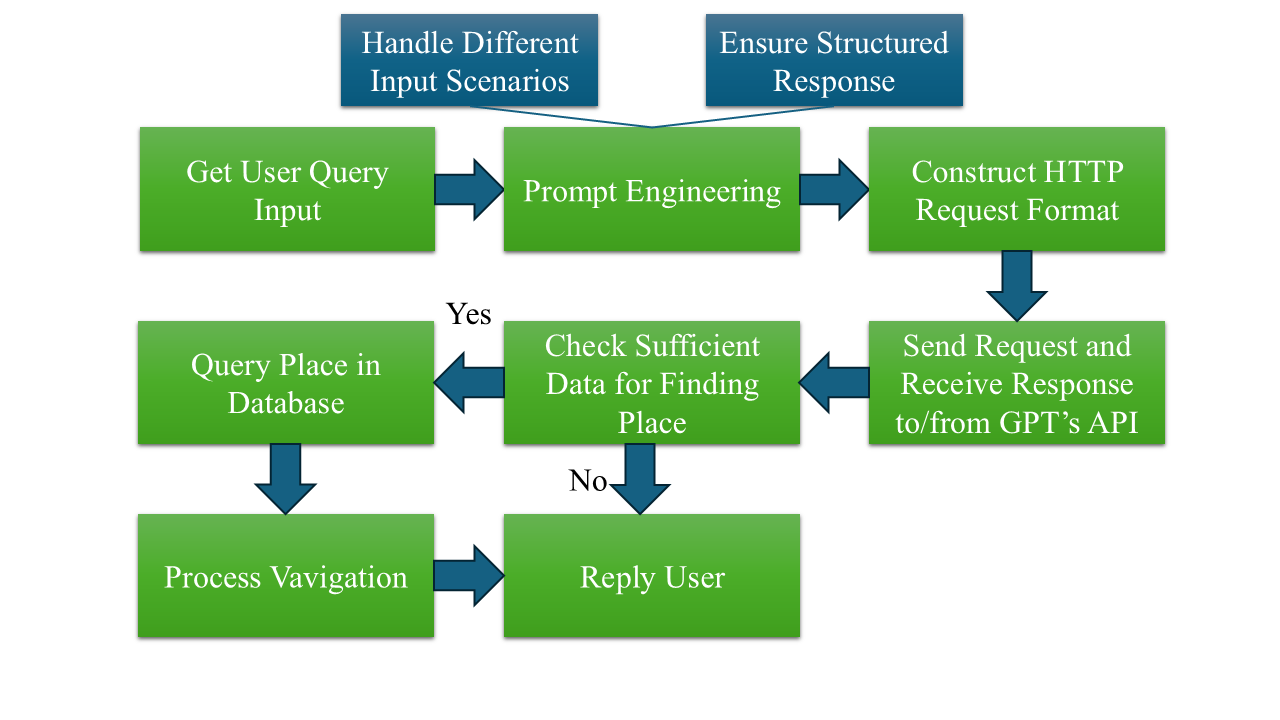
\includegraphics[scale=0.5]{content/resources/images/chap-problems-solutions/ai-assistant-0.PNG}
  \caption{Workflow of building AI Assistant}
  \label{fig:ai-assistant-0}
\end{figure}


% \section{Destination Data Management}\label{sec:DestinationDataManagement}
\subsection{Problem Statement}
To facilitate destination queries, it is necessary to store relevant metadata about each place in a well-organized and accessible manner. For instance, for a room, details such as its building name, room code, purpose, and physical location are essential elements that enable users to narrow down their search quickly and accurately. This metadata is the foundational layer for advanced search functionalities, ensuring that even vague or partial user input can be matched to the correct destination. To manage and retrieve this wealth of information efficiently, building a robust database tailored to the specific needs of destination queries is essential.

\subsection{Solutions}
Large Language Models (LLMs) have revolutionized how natural language is processed by leveraging deep learning architectures trained on vast text corpora. These models excel at understanding context, generating coherent responses, and capturing subtle nuances in language, which make them ideal for interpreting and matching user queries to relevant destination metadata. By integrating LLMs, the solutions can efficiently bridge the gap between unstructured input and structured data, enabling more flexible, accurate, and context-aware search functionalities.

Leveraging the ability of LLMs to process natural language, we have explored three approaches to address this challenge.

\subsubsection{Solution 1: Description Matching}\label{description-matching}
As the most straightforward approach, we store the entire description of each place in the database. When there is a need to query a place, we feed all the place descriptions to the LLMs and ask them to find the best fit. This method ensures that the context is fully preserved, and the correct place is likely to be found most of the time. However, a downside is that it demands substantial storage space. As the number of places increases, storing and searching through large volumes of data becomes expensive and computationally intensive.

\subsubsection{Solution 2: Keyword Matching}
To reduce storage space, for each place we extract and store its most relevant keywords using the LLMs. We apply a reverse index technique, i.e., an edge linking that keyword to the corresponding place is stored for each keyword. Since some keywords are pretty similar (i.e., different keywords describing the same attribute), for example, there might be two rooms with the keywords \texttt{toilet} and \texttt{restroom}, respectively, and the user asks for the nearest \texttt{lavatory}. In this case, both rooms satisfy the query. Therefore, we try to group them under the same keyword. For example, when considering those keywords, \textbf{restroom} can be used uniformly.

To check if the keywords are similar enough to be grouped together, we use vector embeddings. Vector embeddings map words or phrases into a high-dimensional space, where the distance between vectors represents the semantic similarity between their corresponding keywords. We convert each keyword into its vector representation using the LLMs. We then compute the cosine similarity between these vectors to measure how close or related they are. If the similarity score between two keywords exceeds a predefined threshold, we infer that they convey the same or similar meaning, and therefore, we group them under a unified keyword. A sample structure is illustrated in Figure~\ref{fig:data-management-1}.

\begin{figure}[ht]
  \centering
  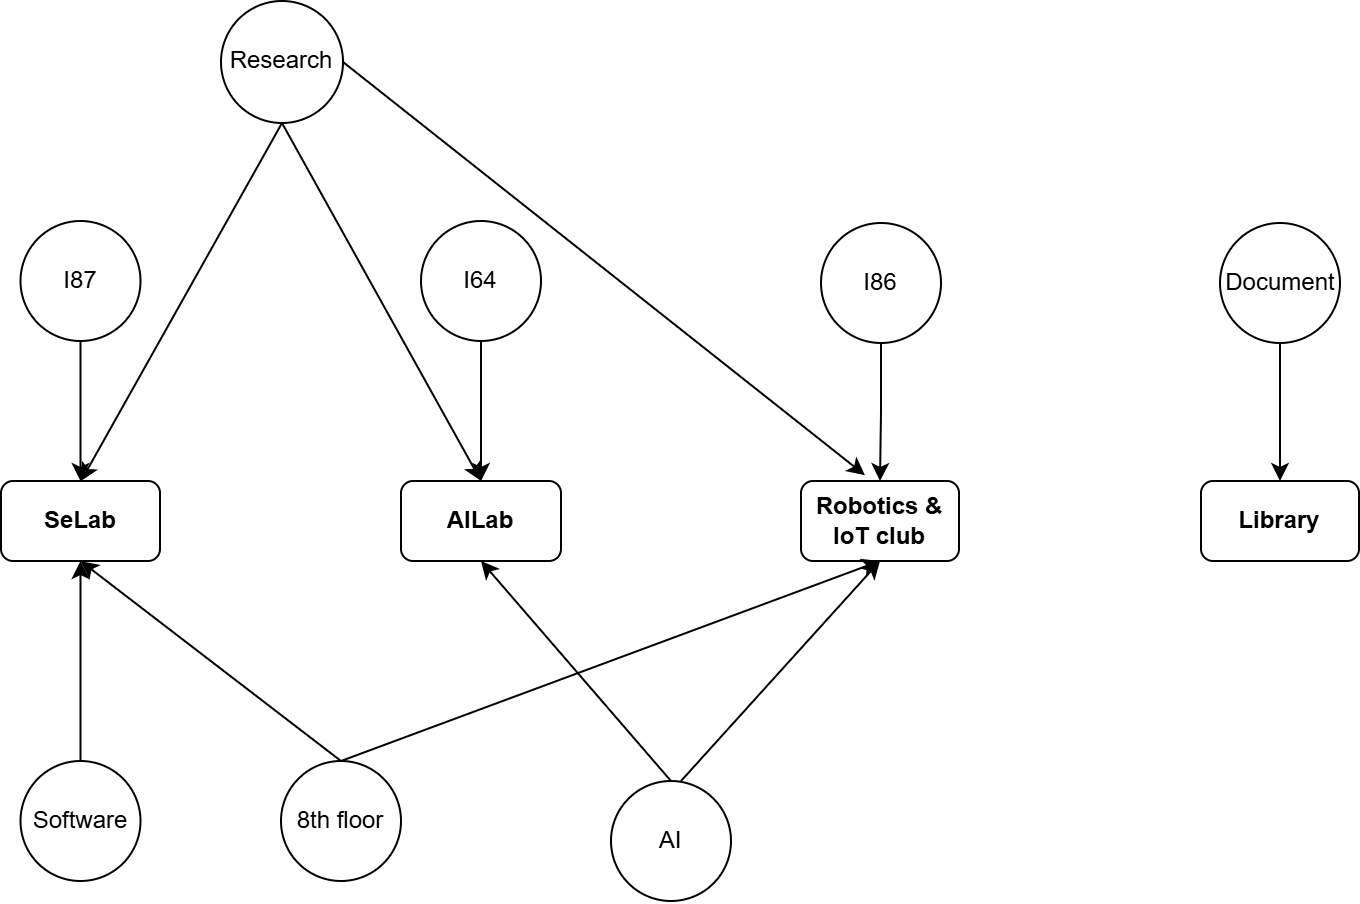
\includegraphics[scale=0.3]{content/resources/images/chap-problems-solutions/data-management-1.png}
  \caption{Keywords graph for four different rooms (square). The keywords are described as nodes (circles).}
  \label{fig:data-management-1}
\end{figure}

When processing a user query for a room, our system first extracts the pertinent keywords. The matching process then involves identifying the room that best corresponds to these keywords. The best match is the room with the highest number of keyword references or ideally contains all the keywords extracted from the query. For instance, if the user provides the following query:

\begin{lstlisting}[style=cSharp]
Please find me the laboratory of software on the 8th level.
\end{lstlisting}

The keywords extracted by the LLM are \texttt{laboratory}, \texttt{software}, and \texttt{8th level}. Using vector embeddings, these can be matched with the defined keys in the database, which are \texttt{research}, \texttt{software}, and \texttt{8th floor}, respectively. Then, the \texttt{SeLab}, \texttt{AILab}, and \texttt{Robotics \& IoT club} are referenced three times, twice, and once, respectively, as shown in Figure~\ref{fig:data-management-2}. Therefore, the \texttt{SeLab} is the desired destination.

\begin{figure}[ht]
  \centering
  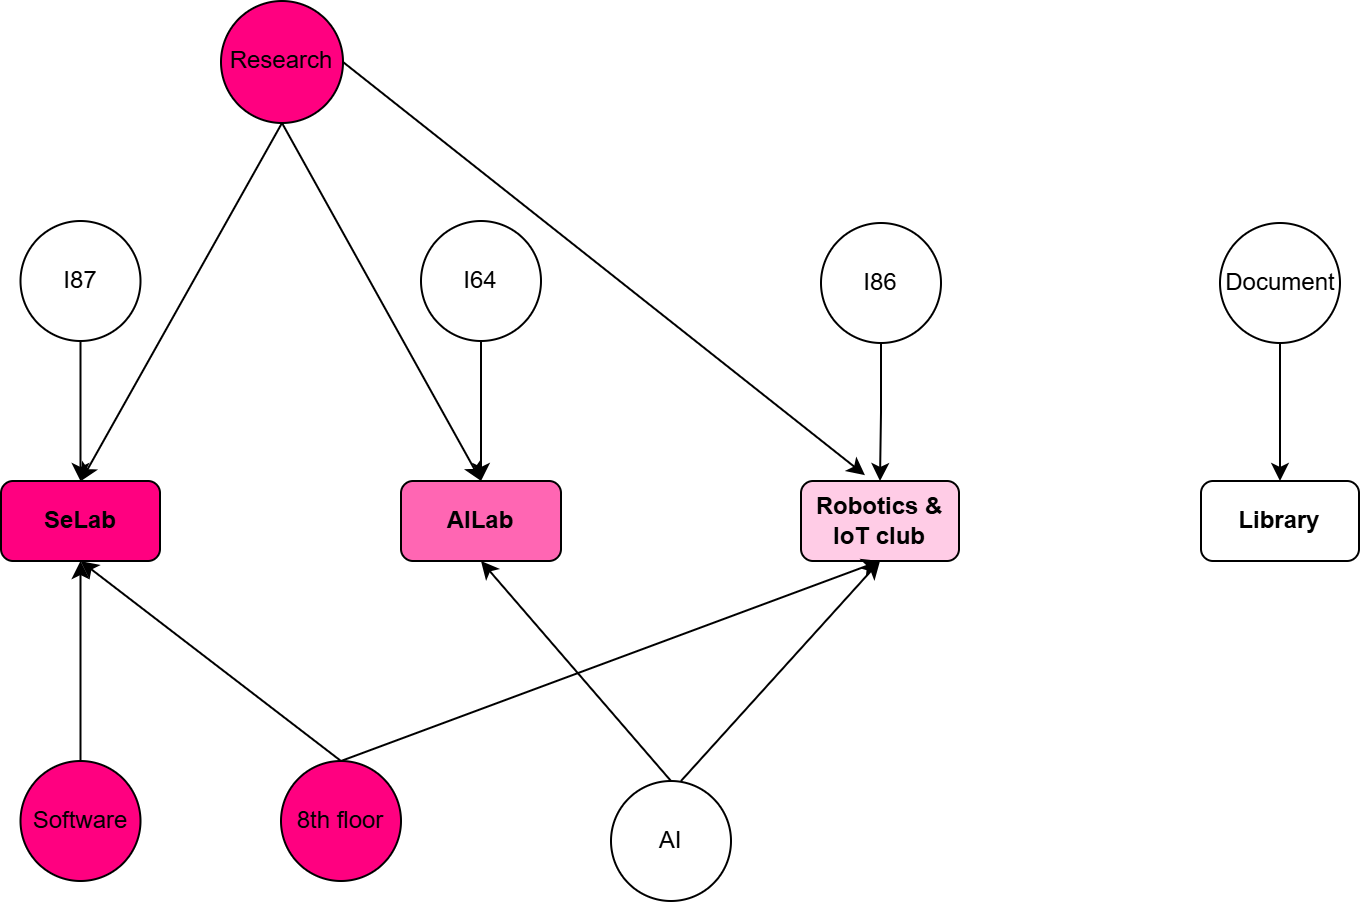
\includegraphics[scale=0.3]{content/resources/images/chap-problems-solutions/data-management-2.png}
  \caption{Reference to rooms with keywords.}
  \label{fig:data-management-2}
\end{figure}

While this approach is efficient in terms of storage and retrieval, it does have certain limitations. A notable downside is that relying solely on keywords may not capture all the nuanced contextual information that can be crucial for an accurate match. As such, manual updates or additional context-aware mechanisms may be required regularly to maintain the system’s accuracy and relevance.

For example, consider a scenario where a user intends to locate the \texttt{Robotics \& IoT club} room but describes it in a less conventional manner:

\begin{lstlisting}[style=cSharp]
Please find me the laboratory next to the I87 room.
\end{lstlisting}

In this case, the LLM extracts the keywords \texttt{laboratory} and \texttt{I87 room}. However, based on our current matching system, these keywords would incorrectly favor the \texttt{SeLab} room. The primary reason for this misinterpretation is that the context in the description is not fully considered. Instead of correctly interpreting “next to the I87 room” as a spatial relation, the system merely processes the keywords. It assumes the target room is the one directly associated with \texttt{I87 room}. Even if we try to extract the keyword as "next to the I87 room", it will either be accurately matched to the keyword "I87" or will not be matched to any of the keywords, resulting in no information gain. \label{no-information-gain}

Another disadvantage is that, since the keywords are scattered, a more general query might not yield any useful information. For example, consider the following query:

\begin{lstlisting}[style=cSharp]
Please navigate me to the laboratory for Computer Science.
\end{lstlisting}

Although both \texttt{AI} and \texttt{software} topics are in the \texttt{Computer Science} category, the initial description might not explicitly state this, and thus there is no such keyword. Therefore, if there are more laboratories in other fields such as Math or Physics, the current data structure cannot be differentiated, although it should be able to be based on the data.\label{not-generalized}

These examples highlight the need for integrating additional context analysis and structuring the data to make the most of the available information and user queries.

\subsubsection{Solution 3: Hierarchical Database with LLM-Driven Question-Answer Metadata scheme}

\subsubsubsection{LLM-Driven Question-Answer Metadata scheme}\label{subsubsub:QA-pairs}
To address the mentioned challenges, we employ an LLM-Driven Question-Answer Metadata scheme. Under this scheme, each place description is processed by the LLMs to generate a set of question-answer pairs that concisely capture the key characteristics of the place. For example, given the following description:

\begin{lstlisting}[style=cSharp]
SELAB was established in 2002 as a pioneer laboratory on software engineering to develop useful systems and services. The research group focuses on the convergence of Artificial Intelligence, Software Engineering, and Human-Computer Interaction to develop smart and secure interactive environments to better assist people in daily lives. SELAB is home to researchers with interests ranging in Machine Learning, Computer Vision, Software Engineering and Human-Computer Interaction.
We welcome students of all levels to take part in our research projects and activities.
Address: I87, 227 Nguyen Van Cu Street, Ward 4, District 5
Ho Chi Minh City
Vietnam
Email:  
contact@selab.hcmus.edu.vn
\end{lstlisting}

The model produces a set of Q\&A pairs like:

\begin{lstlisting}[style=cSharp]
Q: What is the name of the place described?
The name of the place is SELAB.
Q: What is the room code of SELAB?
The room code is I87.
Q: Where is SELAB located?
It is located at 227 Nguyen Van Cu Street, Ward 4, District 5, Ho Chi Minh City, Vietnam.
Q: What is the main purpose of SELAB?
It is a pioneer laboratory on software engineering to develop useful systems and services.
Q: When was SELAB established?
It was established in 2002.
Q: What research fields are focused on at SELAB?
They focus on Artificial Intelligence, Software Engineering, and Human-Computer Interaction.
...
\end{lstlisting}

This approach offers a significantly richer context than traditional keyword matching techniques. The scheme facilitates a more granular understanding of the content by breaking down the full narrative into discrete, focused elements. The generated Q\&A pairs not only summarize the essential details but also capture subtle nuances and interrelationships within the data.

The automation of this process is enabled by LLMs, specifically OpenAI’s GPT in our application, which has been fine-tuned to comprehend and extract contextually relevant information from extensive textual inputs. We developed an application for this purpose, which effectively converts comprehensive place descriptions into well-structured Q\&A metadata. Below is the \hyperlink{prompt-engineering}{prompt} for generating Q\&A pairs.

\begin{lstlisting}[style=cSharp]
This is the description of a place in the university.
Please provide some (sufficient enough) question-answer pairs based on the description below, each pair answering a unique attribute that can be used for finding this place.
Some pivotal information are room code, name, building which it is located, and the purpose of the room, meaning they must be asked if exist in the description.
Please answer EXACTLY 2 * N LINES, each 2 lines are a question and an answer, no more, no less, no any blank lines between, no formatting.
Description: 
\end{lstlisting}

This prompt is designed to enforce strict formatting and ensure the extraction of key details. It instructs the LLM to:
\begin{itemize}
    \item Generate exactly N question-answer pairs (resulting in 2 * N lines of output), with each pair comprising two consecutive lines: one for the question and one for the answer.
    \item Ensure that the pairs sufficiently capture the information needed for querying.
    \item Ensure that each pair corresponds to a specific piece of information.
    \item Ensure that pivotal information—such as the room code, room name, building in which it is located, and the room’s purpose—is included if available in the description.
    \item Produce the output with no additional formatting or blank lines, thereby maintaining a consistent, easily parsable structure for subsequent storage and retrieval in the database.
\end{itemize}

These pairs are then stored in a dedicated database and processed to be added to the hierarchical data structure as discussed in Paragraph~\ref{para:Hierarchical-Database}. Each place is an object in the database containing the Q\&A pairs, position, and id. The id is later used for retrieving the full description if needed, as discussed in Paragraph~\ref{para:Hierarchical-Database}. There is also a refinement session and sanity check to guarantee the correct format, as follows: \label{refine-session}

\begin{lstlisting}[style=cSharp]
public string refineResponse(string response) {
    response = Regex.Replace(response, @"[^a-zA-Z0-9 \n\r-]", "").TrimStart(' ', '\n', '\r');
    response = Regex.Replace(response, @"(?<!^|\s)-|-(?!\d)", "");
    response = Regex.Replace(response, @"^\s*$\n|\r", "", RegexOptions.Multiline);
    if (response.Length % 2 != 0) {
        // handle error
    }
    return response;
}
\end{lstlisting}    

\subsubsubsection{Hierarchical Data Structure}\label{para:Hierarchical-Database}

\subsubsubsubsection*{Data Structure Design}
By breaking down place information into distinct question-answer elements, we build a hierarchy to efficiently organize and retrieve the data. A sample overview of the hierarchy is illustrated in Figure~\ref{fig:data-management-3}.

\begin{figure}[ht]
  \centering
  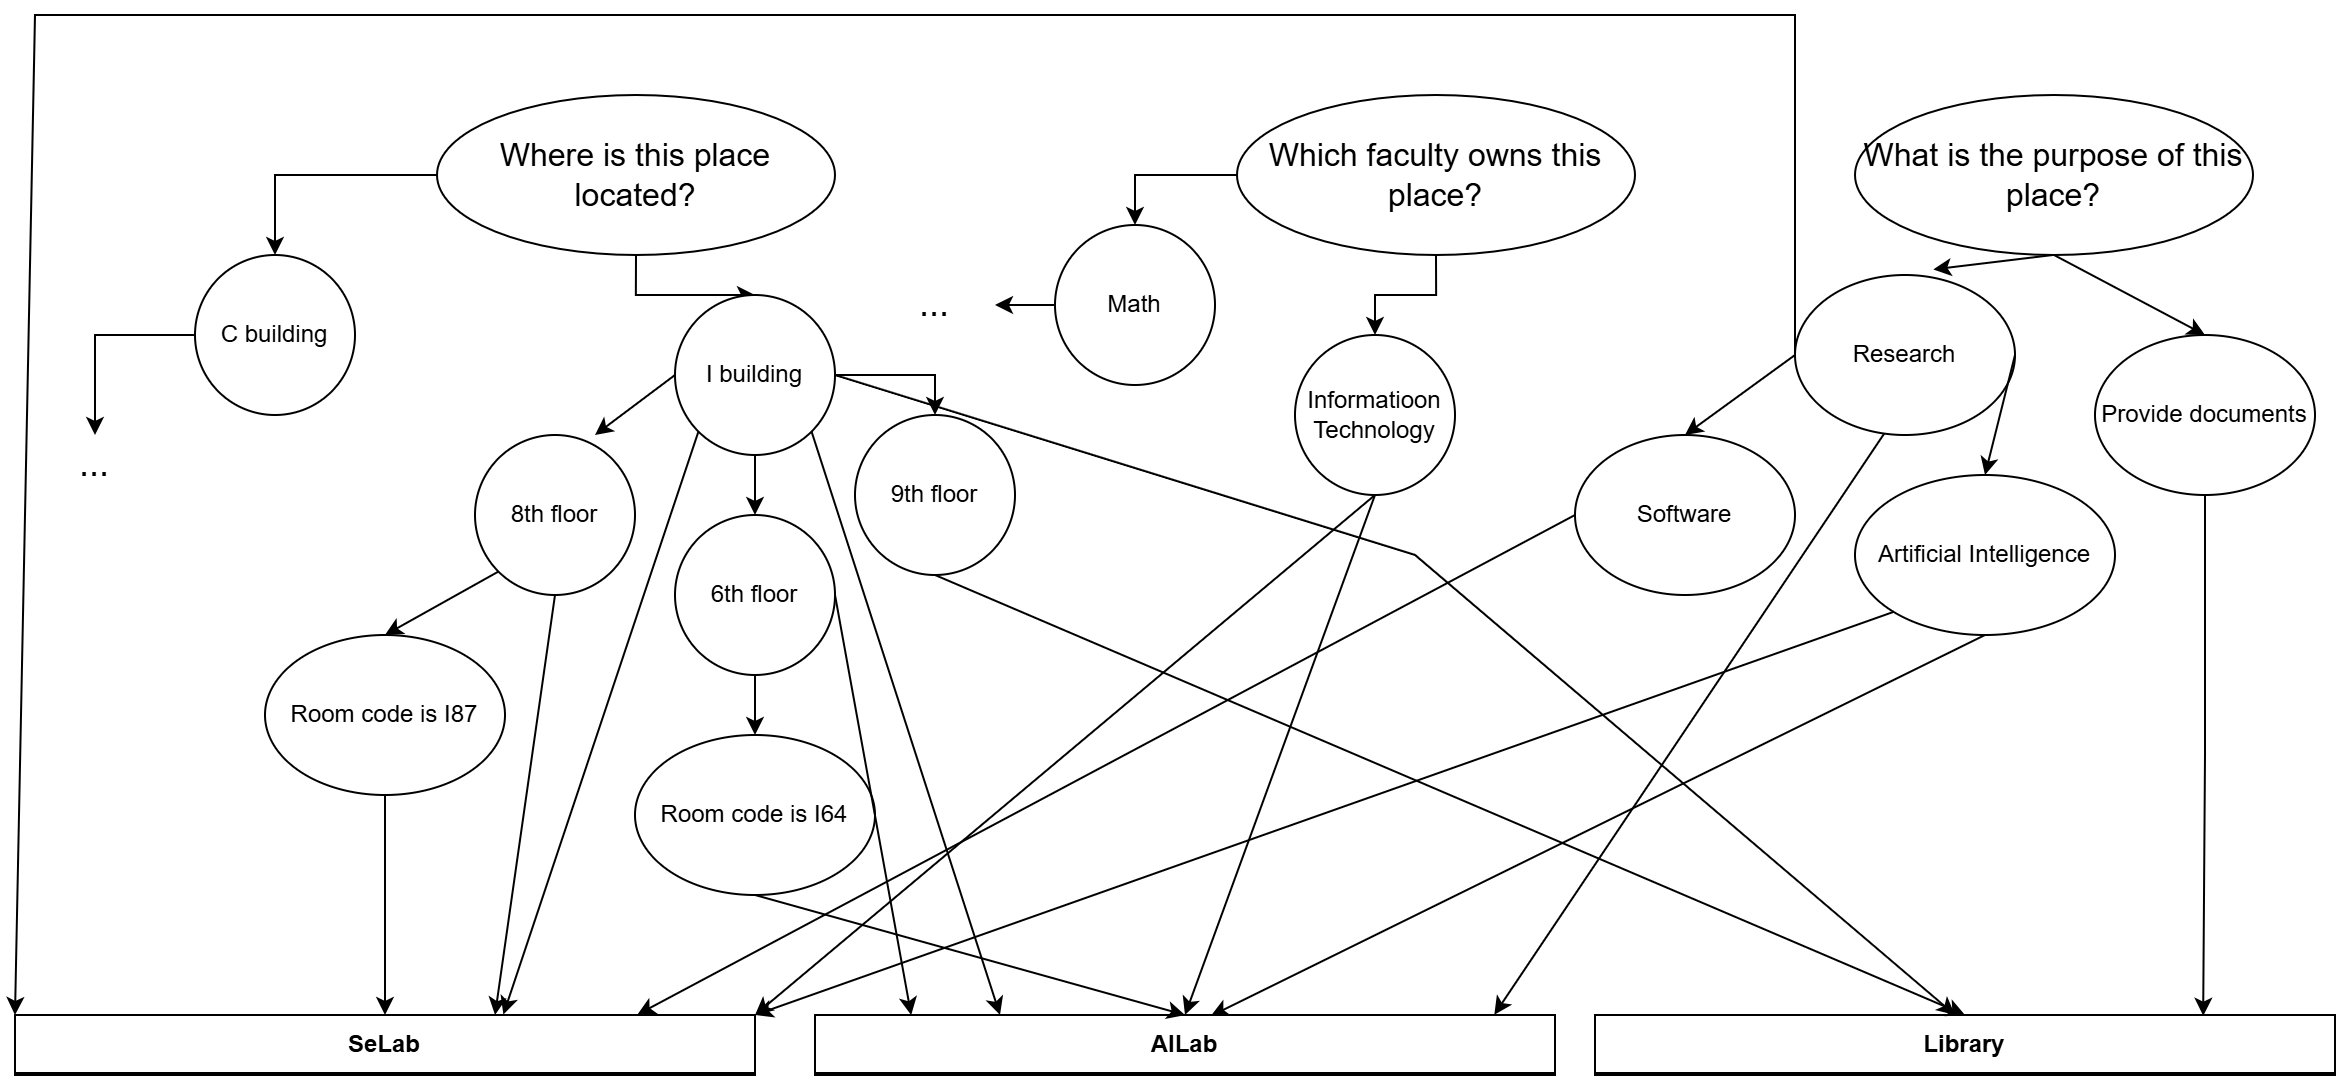
\includegraphics[scale=0.2]{content/resources/images/chap-problems-solutions/data-management-3.png}
  \caption{Hierarchical Data Structure of the three rooms at HCMUS.}
  \label{fig:data-management-3}
\end{figure}

Overall, the hierarchy can be represented as a Directed Acyclic Graph (DAG). We organize places (e.g., SeLab, AILab, Library) according to several attributes. These attributes are grouped under root-level questions, shown at the figure's top. The details are as follows:
\begin{itemize}
\item \textbf{The roots} are the questions pertaining to specific attributes of the places. In other words, each root node corresponds to a fundamental query. These questions do not directly connect to the places; rather, they serve as the entry points for the attribute hierarchy.
\item \textbf{The non-leaf nodes} are the answers for their roots describing the attributes, with the parents containing a generalization of all of their children.
\item \textbf{The leaves} are the actual places themselves (e.g., SeLab, AILab, Library). A leaf node is reached by traversing the path of attributes that fully describe it. The presence of an edge from a non-leaf node to a leaf indicates that the place satisfies the description provided by that node.
\end{itemize}

There is an edge from a non-leaf node to a leaf if the place matches the description in that node. Since a parent contains the generalized description of its children, if there is an edge from a node to a leaf, there must also be an edge from its parent to the leaf, except for the root, as exemplified in Figure~\ref{fig:data-management-4}. With this principle, each attribute can contribute to the finding process at different levels of specificity. For example, if the user asks to find a place with the I87 room, the \texttt{SeLab} can be immediately found (Figure~\ref{fig:data-management-5}). However, suppose the user provides a more vague destination, like finding a room in the I building. In that case, we can still use this information to indicate that the desired destination must be among the three places: \texttt{SeLab}, \texttt{AILab}, or \texttt{Library} (Figure~\ref{fig:data-management-6}). This helps narrow down the search pool of places. Figures~\ref{fig:data-management-7} and~\ref{fig:data-management-8} show the other two common cases.

\begin{figure}[ht]
  \centering
  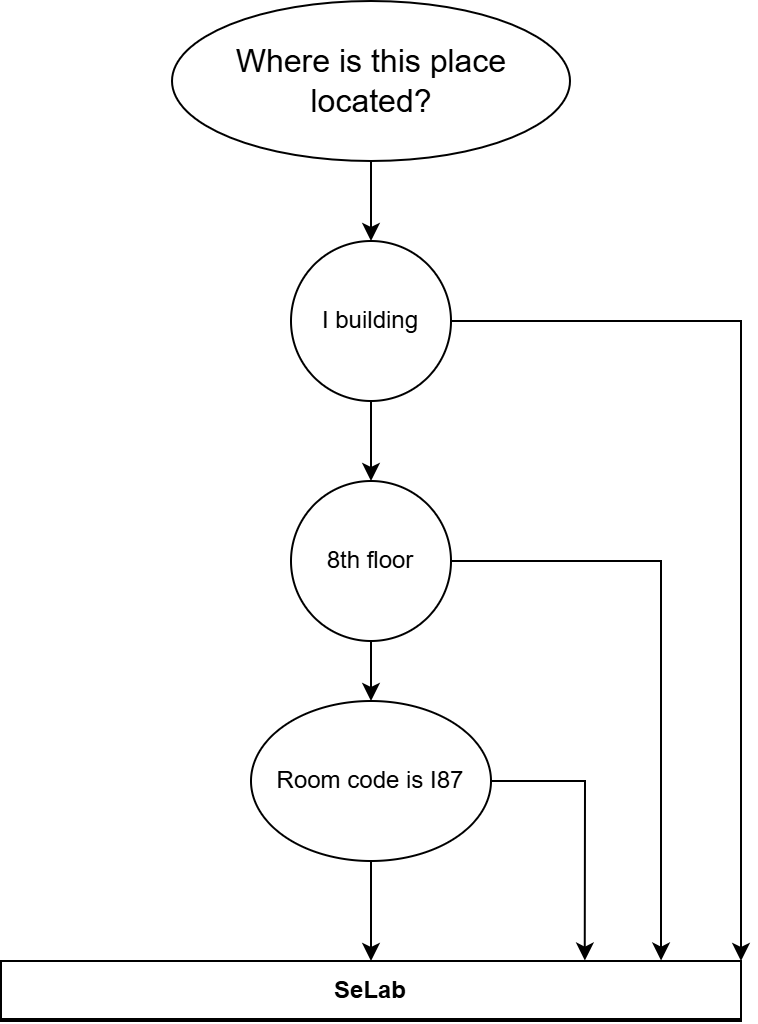
\includegraphics[scale=0.3]{content/resources/images/chap-problems-solutions/data-management-4.png}
  \caption{Leaf's attribute references.}
  \label{fig:data-management-4}
\end{figure}

\begin{figure}[ht]
  \centering
  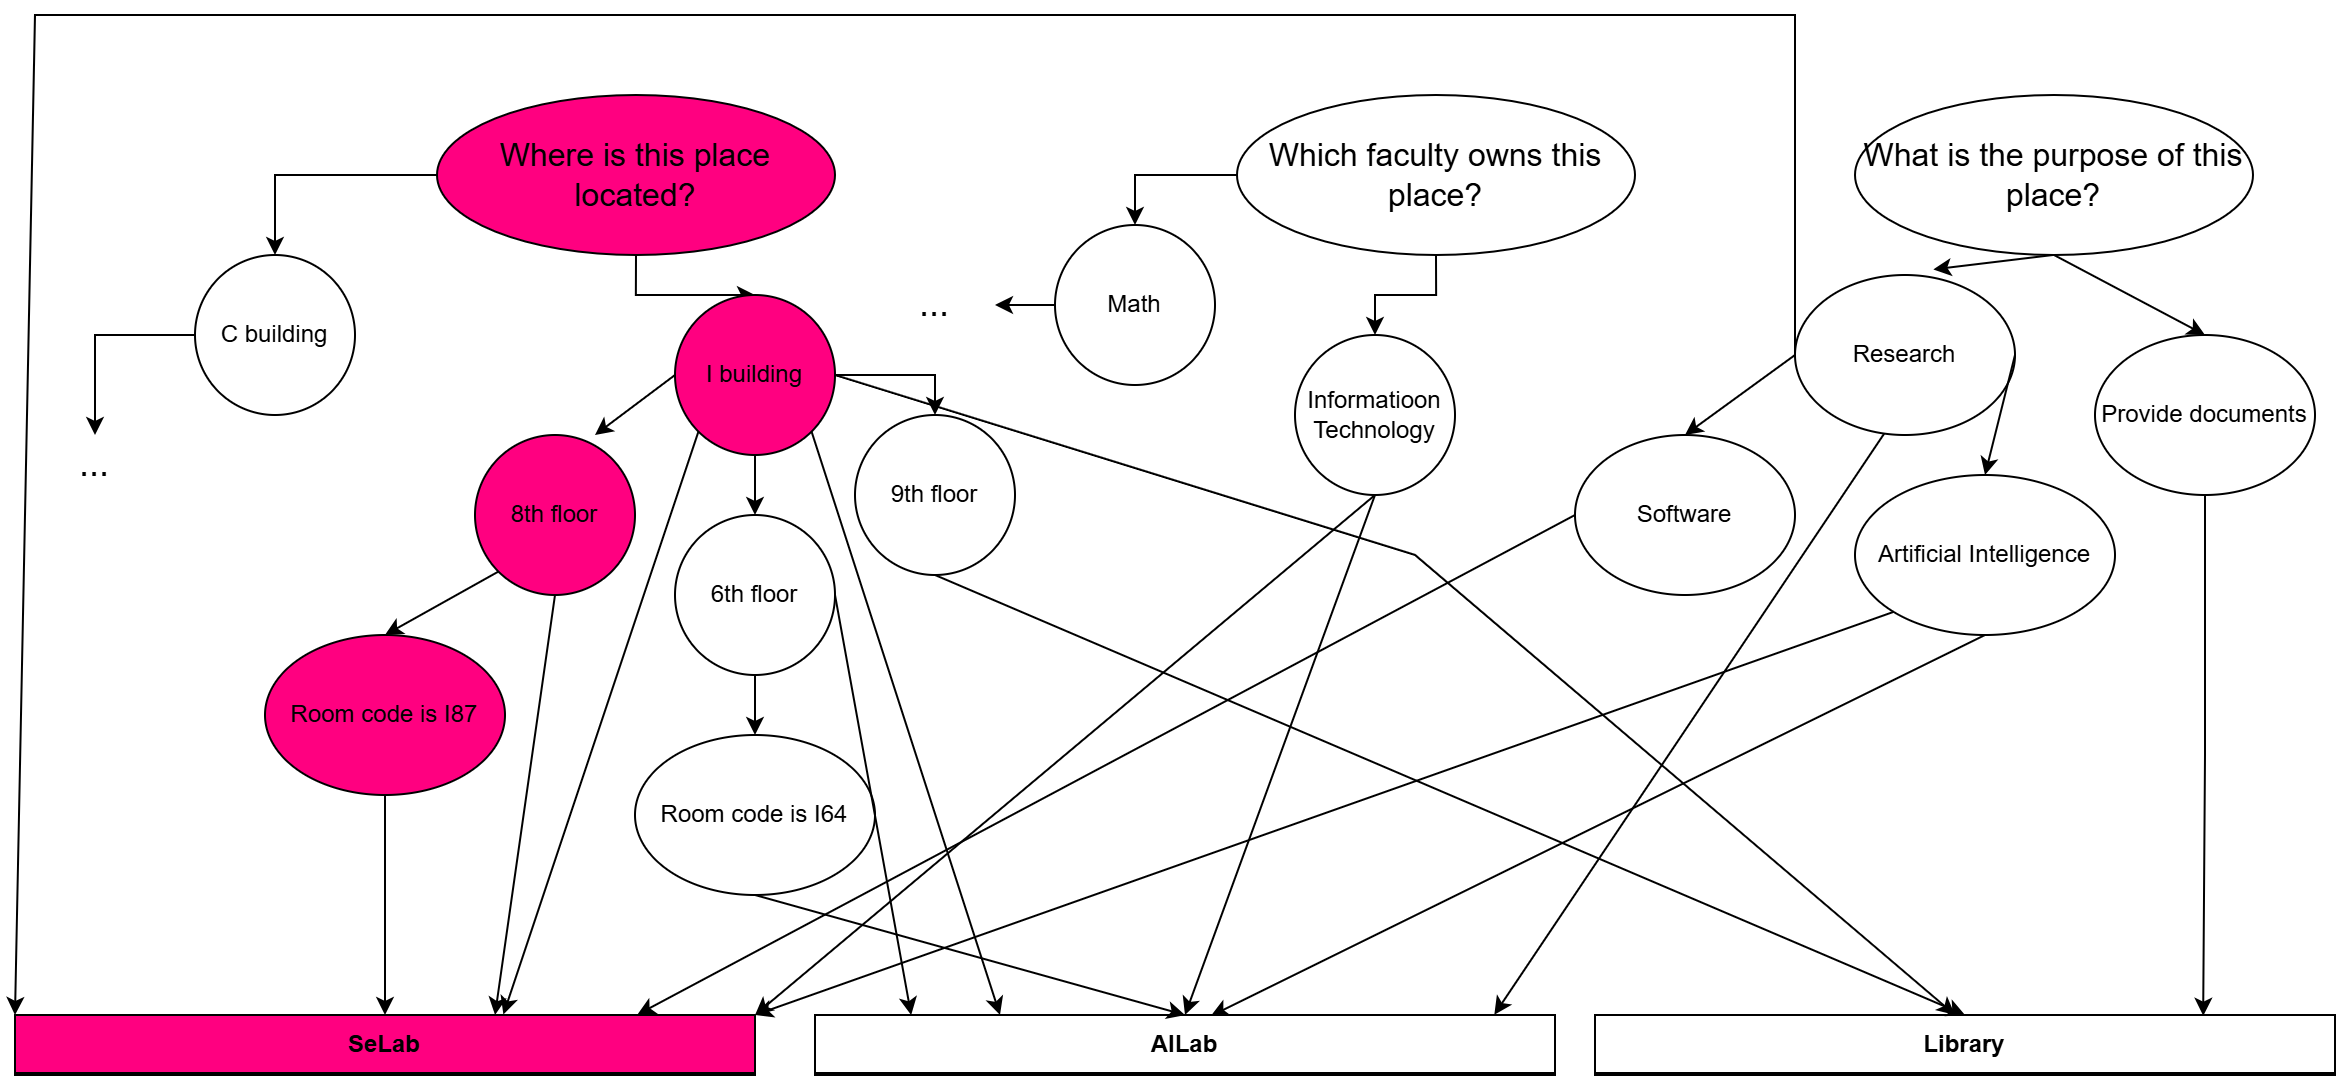
\includegraphics[scale=0.2]{content/resources/images/chap-problems-solutions/data-management-5.png}
  \caption{Find the exact place with detailed information.}
  \label{fig:data-management-5}
\end{figure}

\begin{figure}[ht]
  \centering
  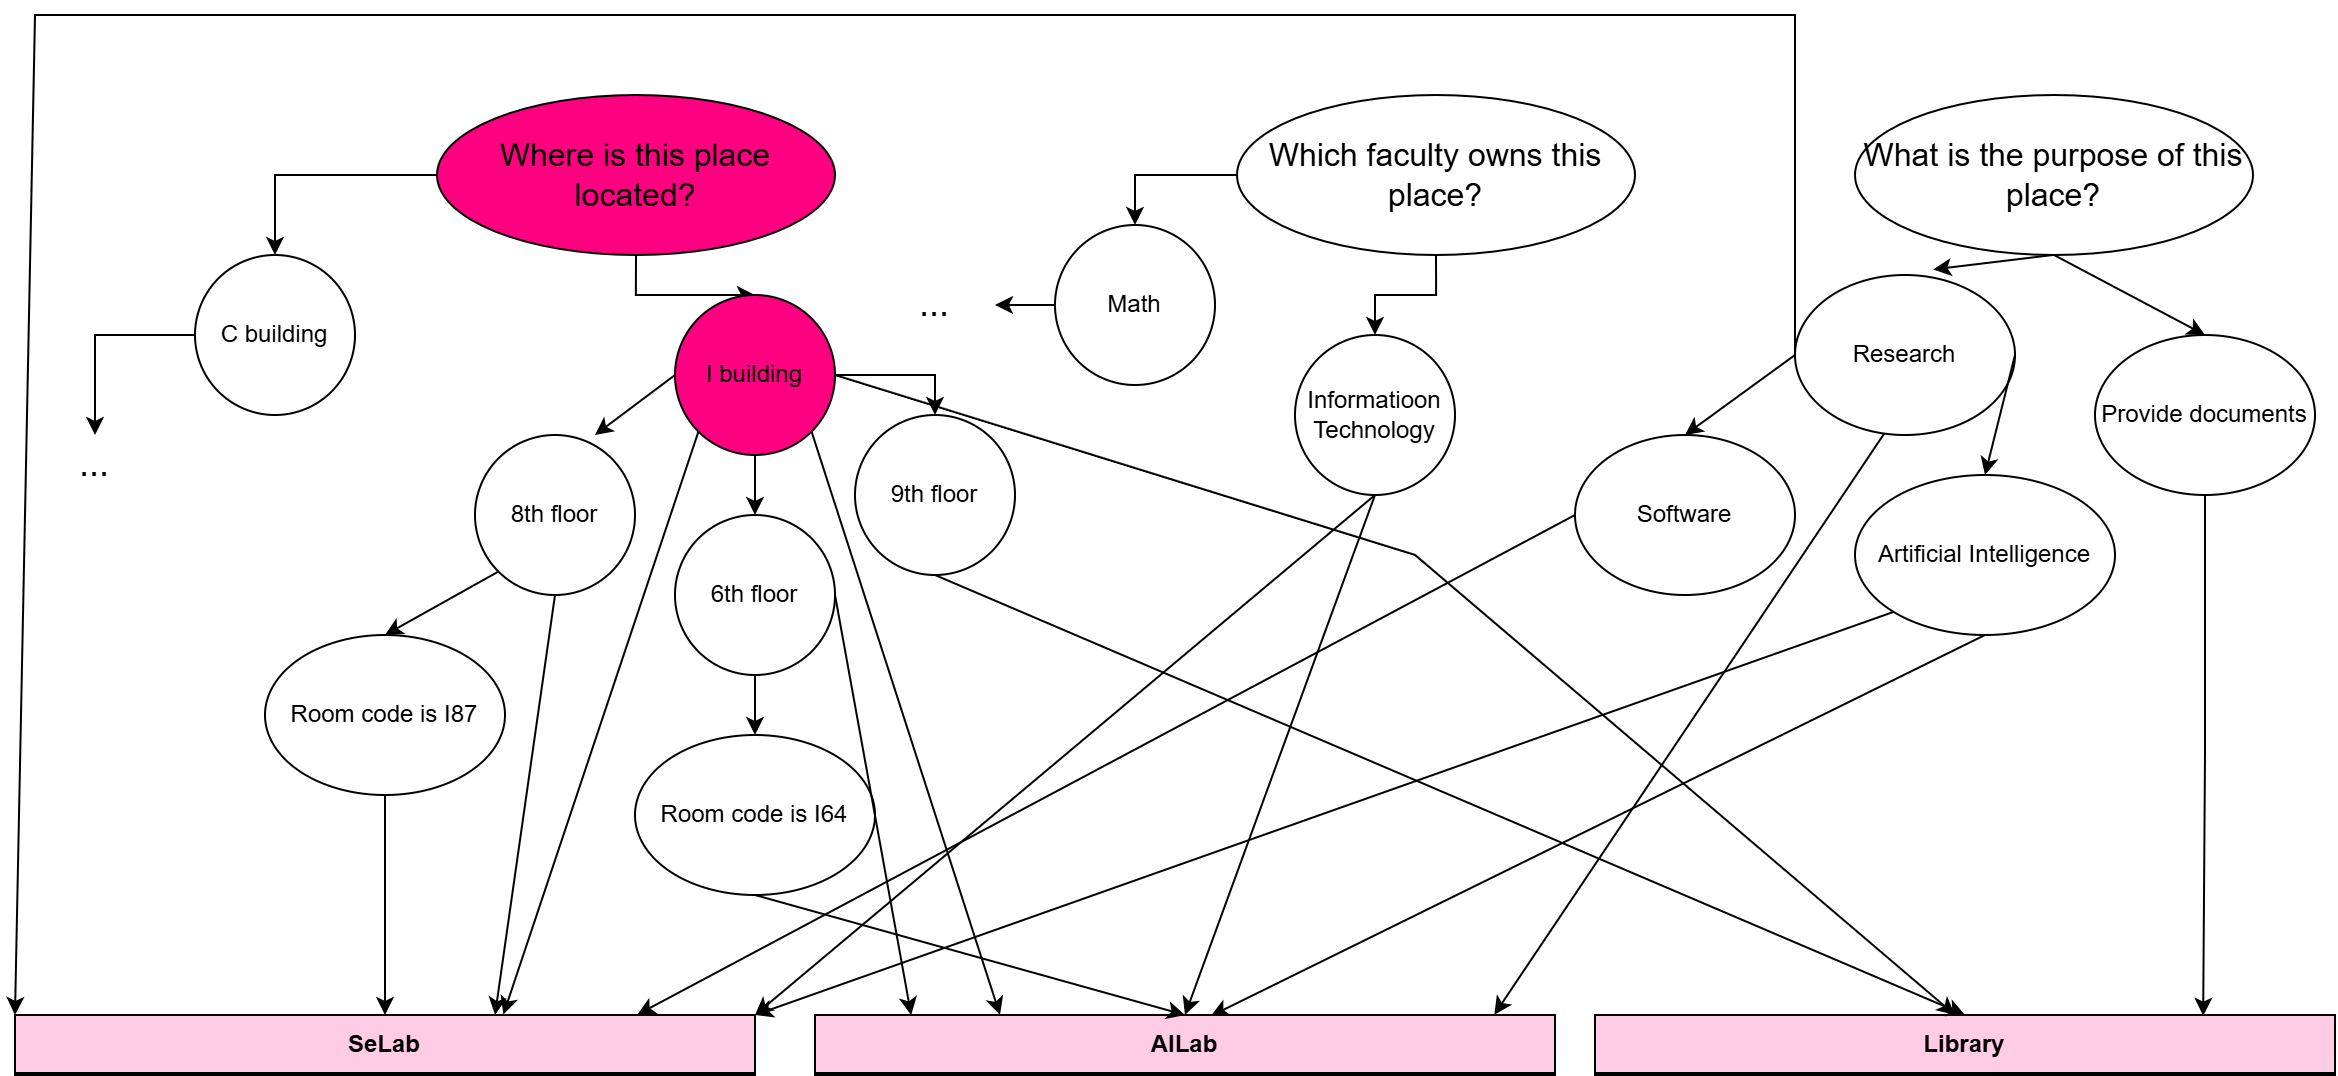
\includegraphics[scale=0.2]{content/resources/images/chap-problems-solutions/data-management-6.png}
  \caption{Narrow down the search range with more generalized information.}
  \label{fig:data-management-6}
\end{figure}

\begin{figure}[ht]
  \centering
  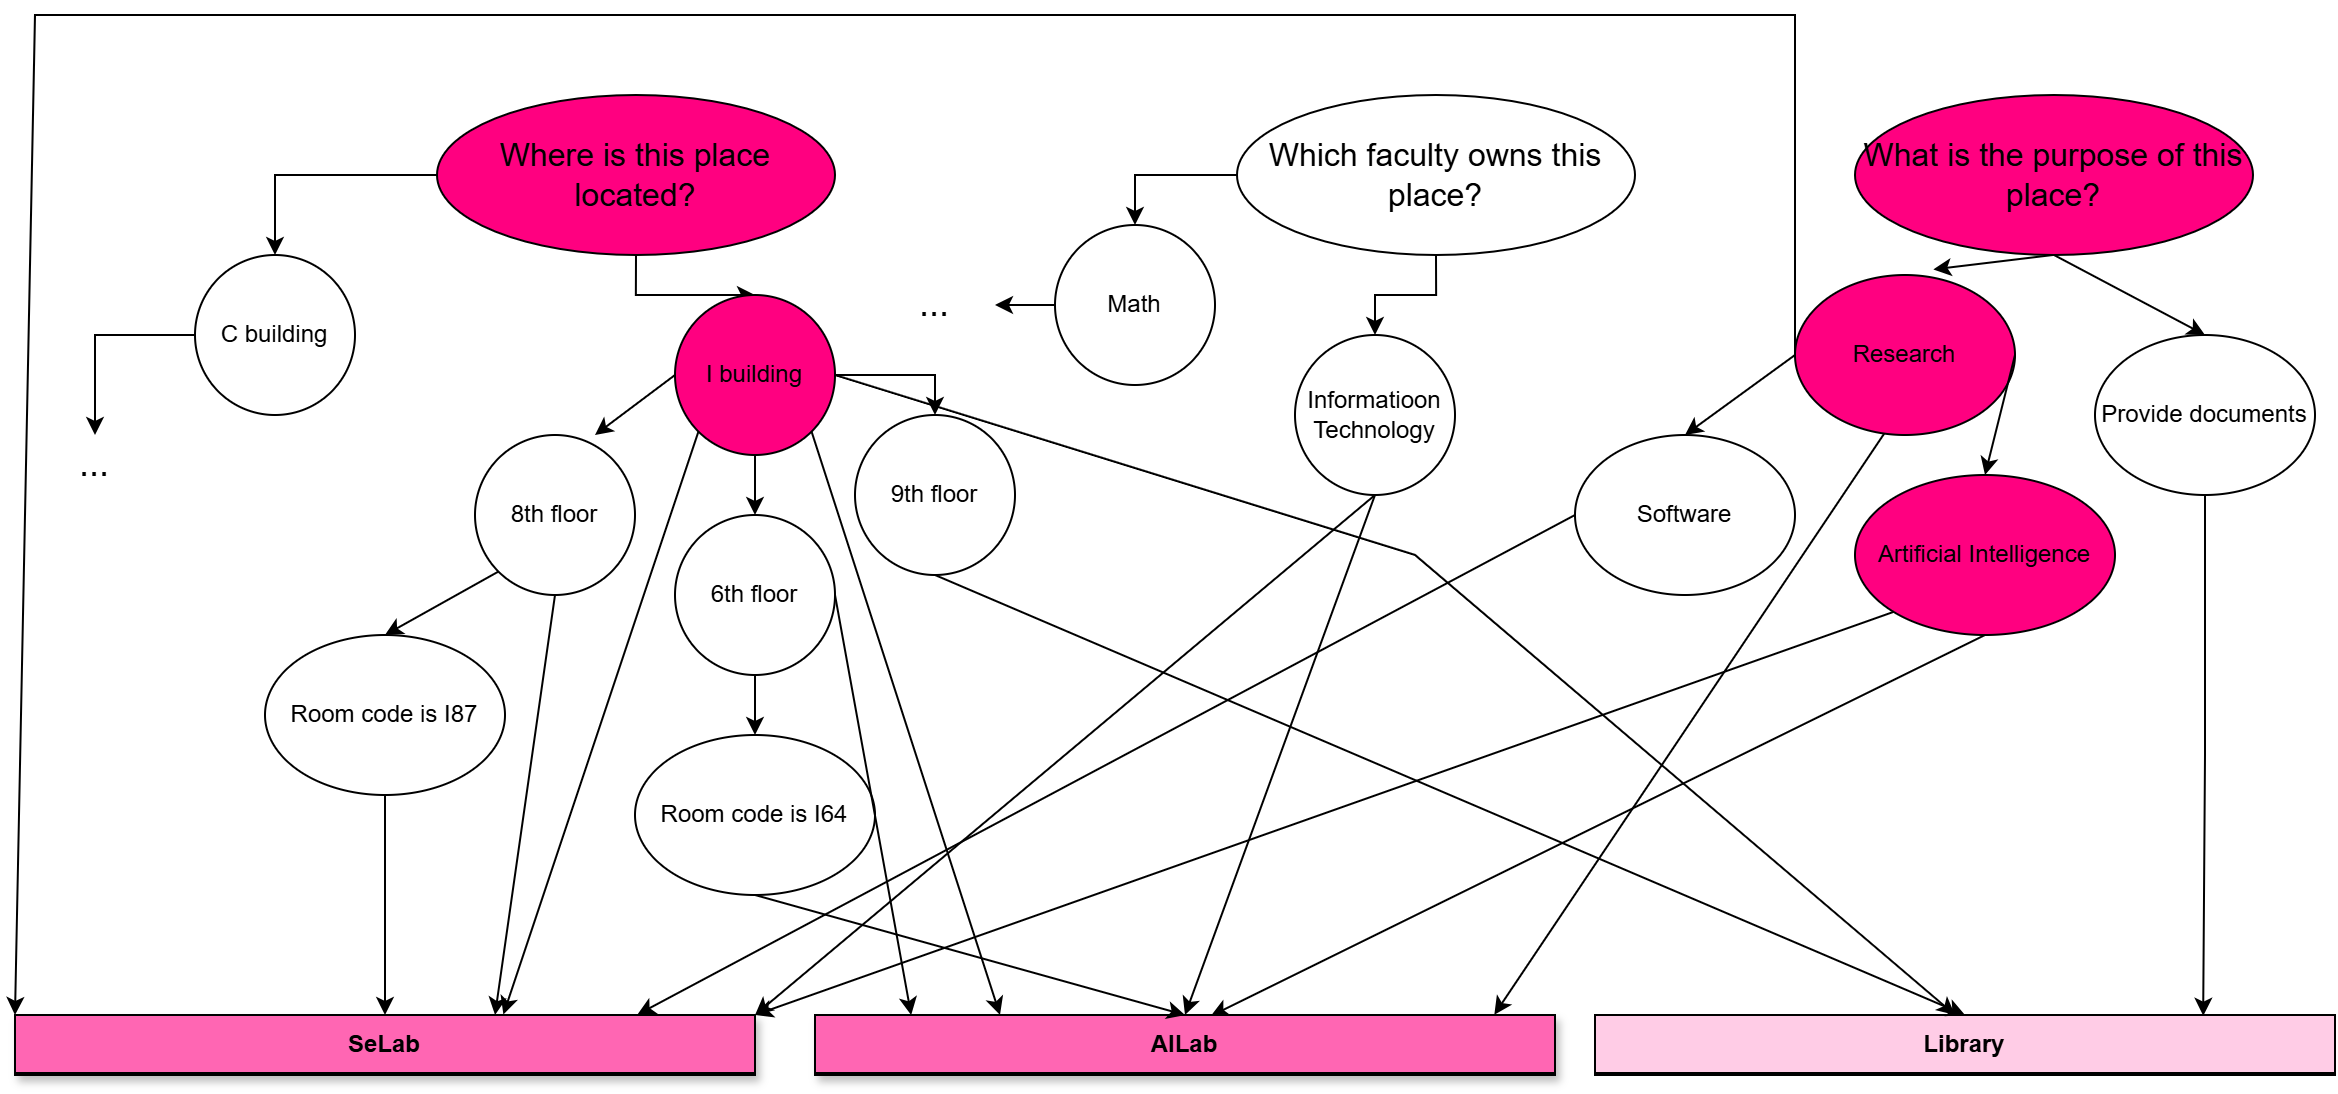
\includegraphics[scale=0.2]{content/resources/images/chap-problems-solutions/data-management-7.png}
  \caption{Narrow down the searching space with \texttt{SeLab} and \texttt{AILab} being the potential candidates.}
  \label{fig:data-management-7}
\end{figure}

\begin{figure}[ht]
  \centering
  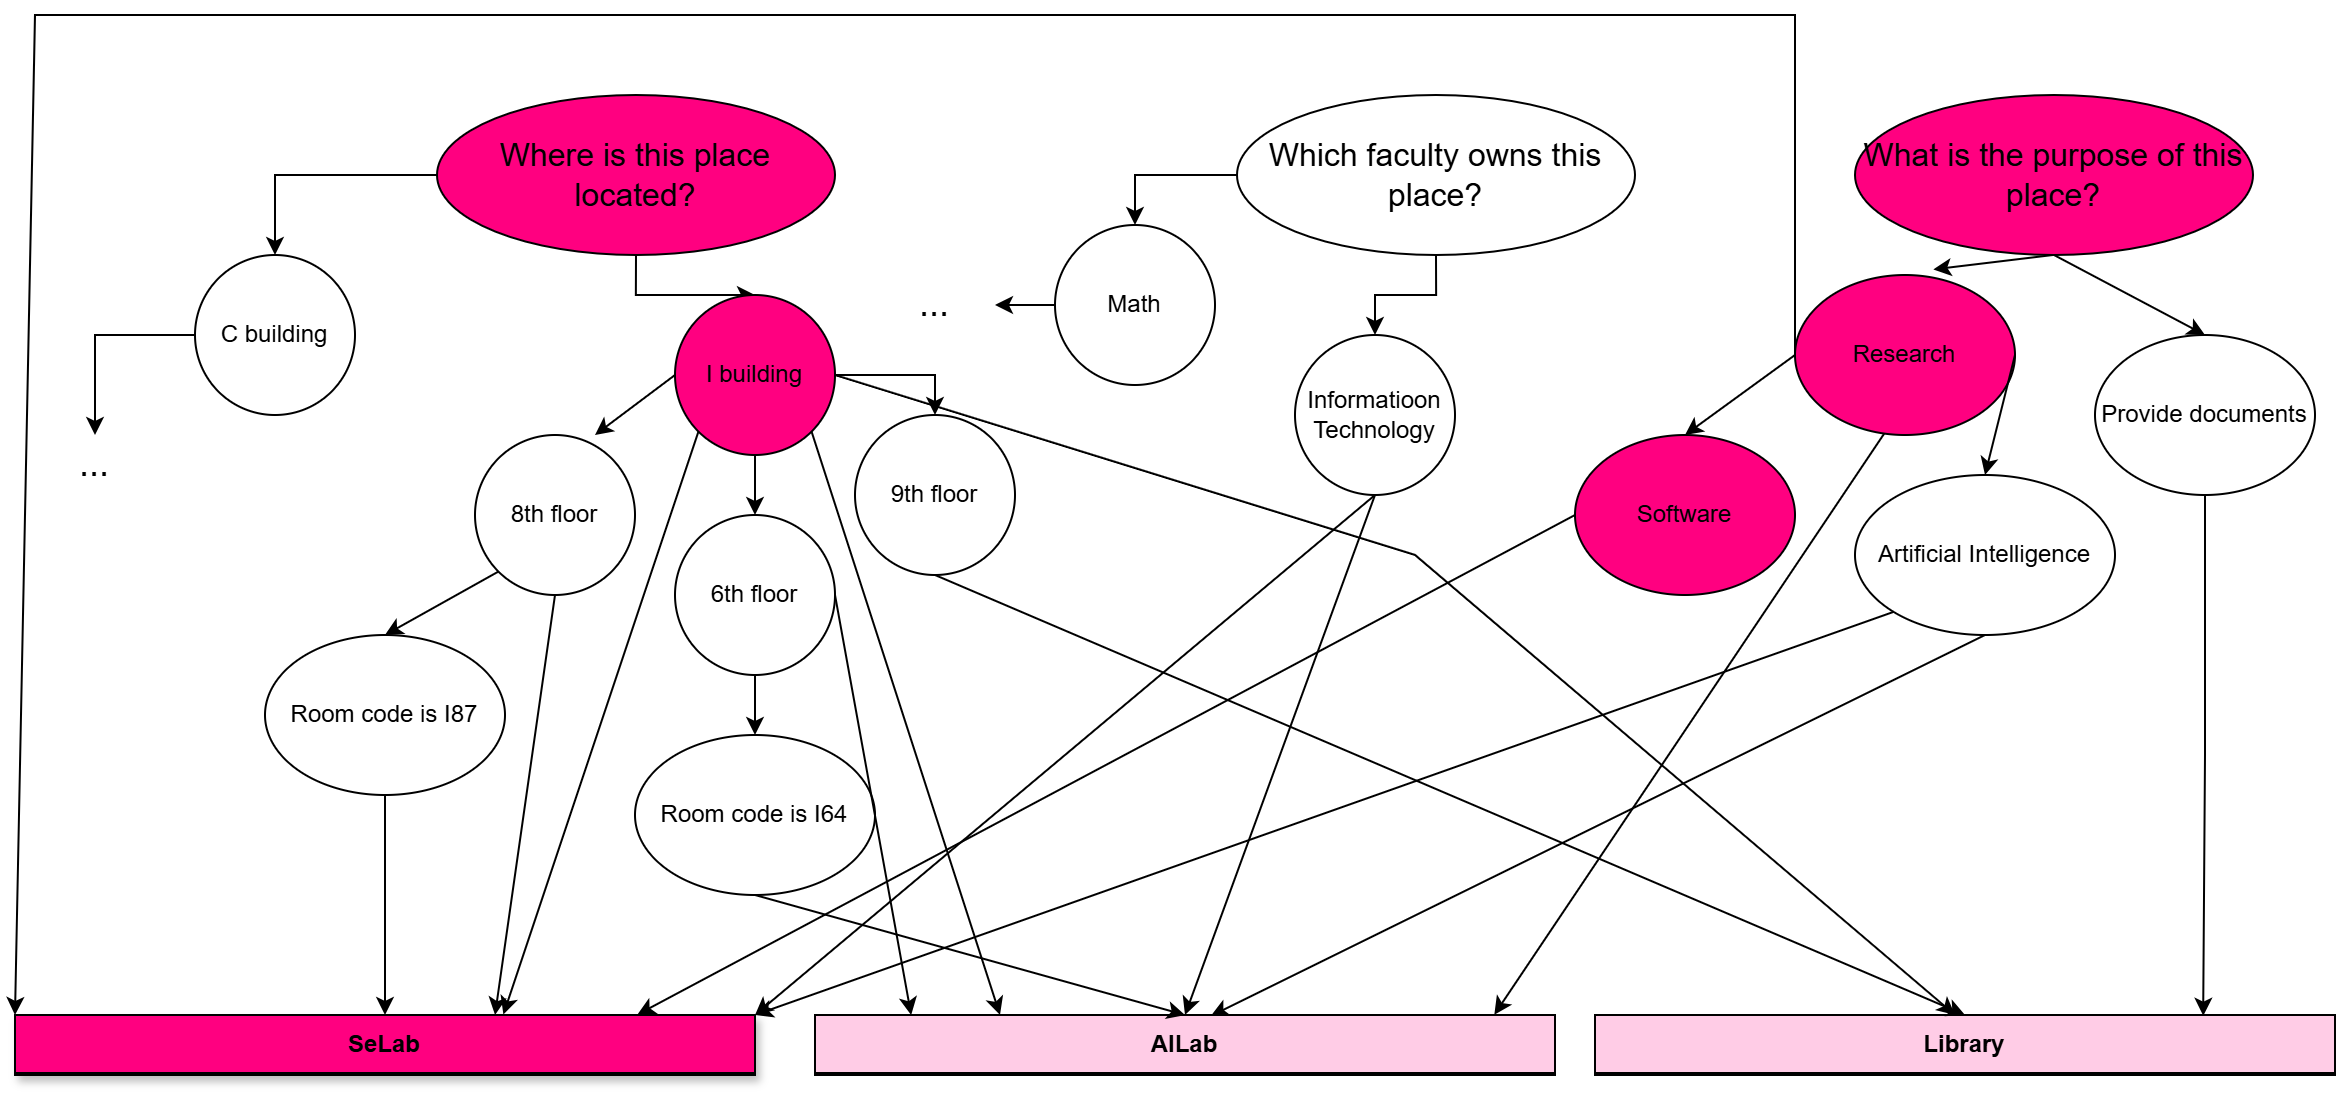
\includegraphics[scale=0.2]{content/resources/images/chap-problems-solutions/data-management-8.png}
  \caption{Searching the exact place with only one most potential candidate being \texttt{SeLab}.}
  \label{fig:data-management-8}
\end{figure}

The hierarchy can be as follows:
\begin{lstlisting}[style=cSharp]
public class HierarchicalDataStructure {
    public const int ROOT = 0;
    public const int SUB_ROOT = 1;
    public const int INTERMEDIATE_NODE = 2;
    public const int LEAF_NODE = 3;
    List<Node> nodes;
}
\end{lstlisting}

A node in the hierarchy can be as follows:

\begin{lstlisting}[style=cSharp]
public class Node {
    public int id;
    public int type;
    public HashSet<int> children;
    public string data;
    public List<String> rules;
}
\end{lstlisting}

The \texttt{id} is the internal id in the hierarchy, which is used for referencing the nodes through a single array \texttt{nodes}. There are four types of nodes, with the \texttt{ROOT} being simply a dummy node for accessing the hierarchy, and the \texttt{SUB\_ROOT}, \texttt{INTERMEDIATE\_NODE}, and \texttt{LEAF\_NODE} corresponding to the roots, non-leaf nodes, and leaves as mentioned above, respectively. The \texttt{children} is the list of links to the lower nodes. The \texttt{data} is:
\begin{itemize}
\item For \texttt{ROOT}: empty, since it is just a dummy node.
\item For \texttt{SUB\_ROOT}: The question that this node represents.
\item For \texttt{INTERMEDIATE\_NODE}: The answer for its \texttt{SUB\_ROOT}, which becomes more specific as one goes downward.
\item For \texttt{LEAF\_NODE}: The information of the place, including its \texttt{id} in the database (as mentioned in Section~\ref{subsubsub:QA-pairs}) for querying the full set of Q\&A pairs if needed. It can also contain some basic information for the place, such as name or position, for immediate usage.
\end{itemize}

The \texttt{rules} is an optional field for the \textt{SUB\_ROOT} only, which is used to define additional rules for each attribute, as discussed in Section~\ref{subsubsubsub:rules}

\subsubsubsubsection*{Query a Place with User's Description}
For a user's description, we also generate the Q\&A pairs. For each pair, we compare the question with the roots to determine if there is a match. If so, we start traversing from that root using the answer in the generated pair to find the most detailed matching attribute. Once we reach the most detailed description possible, we increment the attribute count for all the places referenced. The process is repeated until all pairs are processed, and the place with the highest attribute count will be considered the desired destination. If there are many matching places, we might prompt the user to provide more details about the place, or we might retrieve the complete list of Q\&A pairs for all the found destinations and feed them to the LLM for more detailed matching, as described in Section~\ref{description-matching}. Since the list of places is now much narrower, this operation will be much less costly than previously described.

For now, finding the best matching node is handled through the LLM (specifically ChatGPT's API) to capture the full semantic and contextual meaning best. The nodes are processed by the prompts as follows:
\begin{itemize}
    \item For \texttt{SUB\_ROOT} representing the question, we use the following prompt:
\begin{lstlisting}[style=cSharp]
You are given a pair of text entries: a "Question" and a "Query". Your task is to determine whether the Query provides sufficient information to either directly answer the Question or to allow further classification of potential answers. Follow these rules:
1/ If the Query directly answers the Question, return YES.
2/ If the Query only partially answers the Question but still gives information that can be used to narrow down the possibilities (for example, indicating proximity to a specific room number), return YES.
3/ Otherwise, return NO.
Your output must be exactly one word, either YES or NO, on a single line with no additional text, spaces, or blank lines.
\end{lstlisting}
    \begin{itemize}
        \item Ensure the query accurately matches the question.
        \item Accept the case where the answer might not transparently answer the question but does provide useful information, handling the case mentioned in Section~\ref{no-information-gain}.
        \item Ensure the correct response format.
    \end{itemize}
    
    \item For \texttt{INTERMEDIATE\_NODE} representing an attribute, we use the following prompt:
\begin{lstlisting}[style=cSharp]
You are given a question, a query, and several candidate answers in the format "ID: description". Here, the 'Question' asks for an attribute and the 'Query' is the user’s description of the desired attribute. Following the Query, each line provides a candidate answer where the first candidate is a generalization (i.e., the parent) of all subsequent, more specific answers. Your task is to select the best matching candidate IDs based on the following rules:
1. If the Query is not specific enough and only aligns with the generalization, return only the first candidate's ID.
2. If the Query provides specific information that matches one or more specific candidates, return all matching candidate IDs (each on its own line).
3. If the Query explicitly negates or does not match any candidate when specificity is expected, return an absolutely empty message.
4. If there is an exact match, return only that candidate's ID.
5. If the Query is vague but still permits multiple possibilities, return all candidate IDs that could be valid given the Query, excluding any that are explicitly ruled out.

Your output must contain only the matching candidate IDs (or nothing — an absolutely empty message), with each ID on a separate line and no extra text, spaces, or blank lines.

Examples:
Example 1 (Exact Match):
Question: What is the purpose of this room?
Query: This room is for software engineer research
2: The room purpose is for researching
4: The room purpose is for software engineer research
17: The room purpose is for biology research
Output:
4

Example 2 (Not Specific Enough):
Question: What is the purpose of this room?
Query: This is a laboratory
2: The room purpose is for researching
3: This room is for software engineer research
4: This room is for biology research
Output:
2

Example 3 (Specific but No Match):
Question: What is the purpose of this room?
Query: This room is for math research
2: The room purpose is for researching
3: This room is for software engineer research
4: This room is for biology research
Output:
\end{lstlisting}
    \begin{itemize}
        \item Summarize the context for better contextual handling.
        \item Ensure the query reaches the appropriate level of generalization for the attribute, handling the case mentioned in Section~\ref{not-generalized}.
        \item Correctly utilize other types of information for classifying the nodes, for example, the negation cases, handling the case mentioned in Section~\ref{no-information-gain}.
        \item Exemplify some pivotal cases for accurate handling.
        \item Ensure the correct response format.
    \end{itemize}

\end{itemize}

To confidently ensure the response formats are accurate, all responses will be refined as mentioned in Section~\ref{refine-session}.

For each node, we process it with the following function:

\begin{lstlisting}[style=cSharp]
public async Task TraverseTreeQuery(int id, string query, string sub_root_question = "")
\end{lstlisting}

The details of this function are as follows:
\begin{itemize}
    \item This is a recursive function that is called for each node matching the previous query to traverse further in the hierarchy.
    \item \texttt{id} is the id of the current node being processed.
    \item \texttt{query} is a sentence representing a queried attribute.
    \item \texttt{sub\_root\_question} is the question of the corresponding \texttt{SUB\_ROOT} to capture the context better when matching the query with the answers.
\end{itemize}

When reaching the deepest node (i.e., when it cannot be more specific for the current query), we update the count for places, which are the \texttt{LEAF\_NODE}, as follows:

\begin{lstlisting}[style=cSharp]
foreach (int child in nodes[id].children) {
    if (nodes[child].type == LEAF_NODE) {
        if (matches.ContainsKey(child)) {
            matches[child]++;
        }
        else {
            matches[child] = 1;
        }
    }
}
\end{lstlisting}

Note that a bottleneck in this hierarchy is the response time from the LLM at each node. Although the processed nodes might eventually reference the same leaf nodes, those leaves are also the only shared nodes. Therefore, we consider each node as a separate branch that can be processed concurrently, and thus many requests to the LLM will be sent concurrently, reducing the total response time. Finally, \texttt{ConcurrentDictionary}, a thread-safe hash map in C\#, can handle concurrent leaf node matching. Below is how we use \texttt{Task} for processing the branches concurrently:

\begin{lstlisting}[style=cSharp]
List<Task> tasks = new List<Task>();

// Traverse the tree
foreach (int child in nodes[root].children) {
    foreach (string query in queries) {
        tasks.Add(TraverseTreeQuery(child, query));
    }
}
await Task.WhenAll(tasks);
\end{lstlisting}

Below is an example of processing a query (Figure~\ref{fig:data-management-8}). Consider the query:

\begin{lstlisting}[style=cSharp]
Find me the software lab in I building. 
\end{lstlisting}

The generated pairs are:

\begin{lstlisting}[style=cSharp]
What is the purpose of this room?
This room is a software laboratory.
What is the building of this room?
This room is in the I building.
\end{lstlisting}

Comparing each pair of questions from \texttt{SUB\_ROOT} nodes and the generated ones, we have two matches: \texttt{(What is the location of this lab?, Where is this place located?)} and \texttt{(What is the purpose of this room?, What is the purpose of this room?)}.

For the first question, the LLM then responds with the \texttt{I building} node as the best match. After that, when processing the \texttt{I building} node, the LLM responds that the only match is the \texttt{I building} node, which is the current node itself. This means that we have reached the deepest possible level of specification for this question, given the query; therefore, all of its children, including all three rooms, are marked as matches.

For the second question, the LLM then responds with the \texttt{Research} node as the best match, and then \texttt{Software} as the best match. Since this node has no other \texttt{INTERMEDIATE\_NODE} children, we have reached the deepest level of specification. Therefore, its only child, \texttt{SeLab}, is marked.

Finally, since the only leaf with the highest attribute count, this is the desired destination since \texttt{SeLab} is the only leaf with the highest attribute count.

\subsubsubsubsection*{Add a New Place to the Hierarchy}
First, a new \texttt{LEAF\_NODE} representing the new place is created. Similar to the querying process, using the metadata of the place (i.e., the set of Q\&A pairs), we traverse the existing hierarchy to find any matching attributes and reference them to the new node. When there are no matches, we create a new node with the following prompt:

\begin{lstlisting}[style=cSharp]
I want to build a hierarchy for a room/place in the campus.
Given the following attribute description that is to answer the below question.
Please consider the following two cases:
    1. If the description can be generalized, return the generalized description.
    2. Otherwise, return the description itself.
For example, if the question is ""What is the purpose of this room?"", and the description is ""The room is for computer science research"".
In this case, return ""The room is for research purposes"", since it is more general.
Another example, if the question is ""What is the room number?"", and the description is ""The room number is I87"".
In this case, return ""The room number is I87"", since it cannot be generalized.
Just return description, NO OTHER WORDS OR CHARACTERS.
\end{lstlisting}

This prompt:
\begin{itemize}
    \item Summarizes the context for better contextual handling.
    \item Generates the descriptive data for this node for the new place. If possible, it also attempts to create a generalized description for handling the case mentioned in Section~\ref{not-generalized}.
    \item Correctly utilizes other types of information for classifying the nodes, for example, the negation cases, handling the case mentioned in Section~\ref{no-information-gain}.
    \item Exemplifies some pivotal cases for accurate handling.
    \item Ensures the correct response format.
\end{itemize}

For example, consider adding a place with the following Q\&A pairs metadata:

\begin{lstlisting}[style=cSharp]
What is the purpose of this place?
The purpose of this place is for researching microbiology.
Which faculty does this place belong to?
This place belongs to the Biology Faculty.
\end{lstlisting}

The hierarchy is updated as in Figure~\ref{fig:data-management-9}. In this figure, the pink nodes are the nodes that matched the new place's attributes, while the blue ones are the newly created nodes. As we can see, three common cases are being exemplified here:
\begin{itemize}
\item The questions and the \texttt{Research} node are reused since those match the new attributes.
\item The \texttt{Biology} node (the one under the \texttt{Which faculty owns this place?} node) is created as described in the metadata.
\item The \texttt{Biology} node (the one under the \texttt{Research} node), although not explicitly described in the metadata, is created as a generalization of the \texttt{Microbiology} attribute. This node guarantees the structure of the hierarchy.
\end{itemize}

Using this method in combination with the Q\&A pairs generation mentioned in Section~\ref{subsubsub:QA-pairs}, the entire process of adding a new place with a raw description to the data structure can be fully automated.

\begin{figure}[ht]
  \centering
  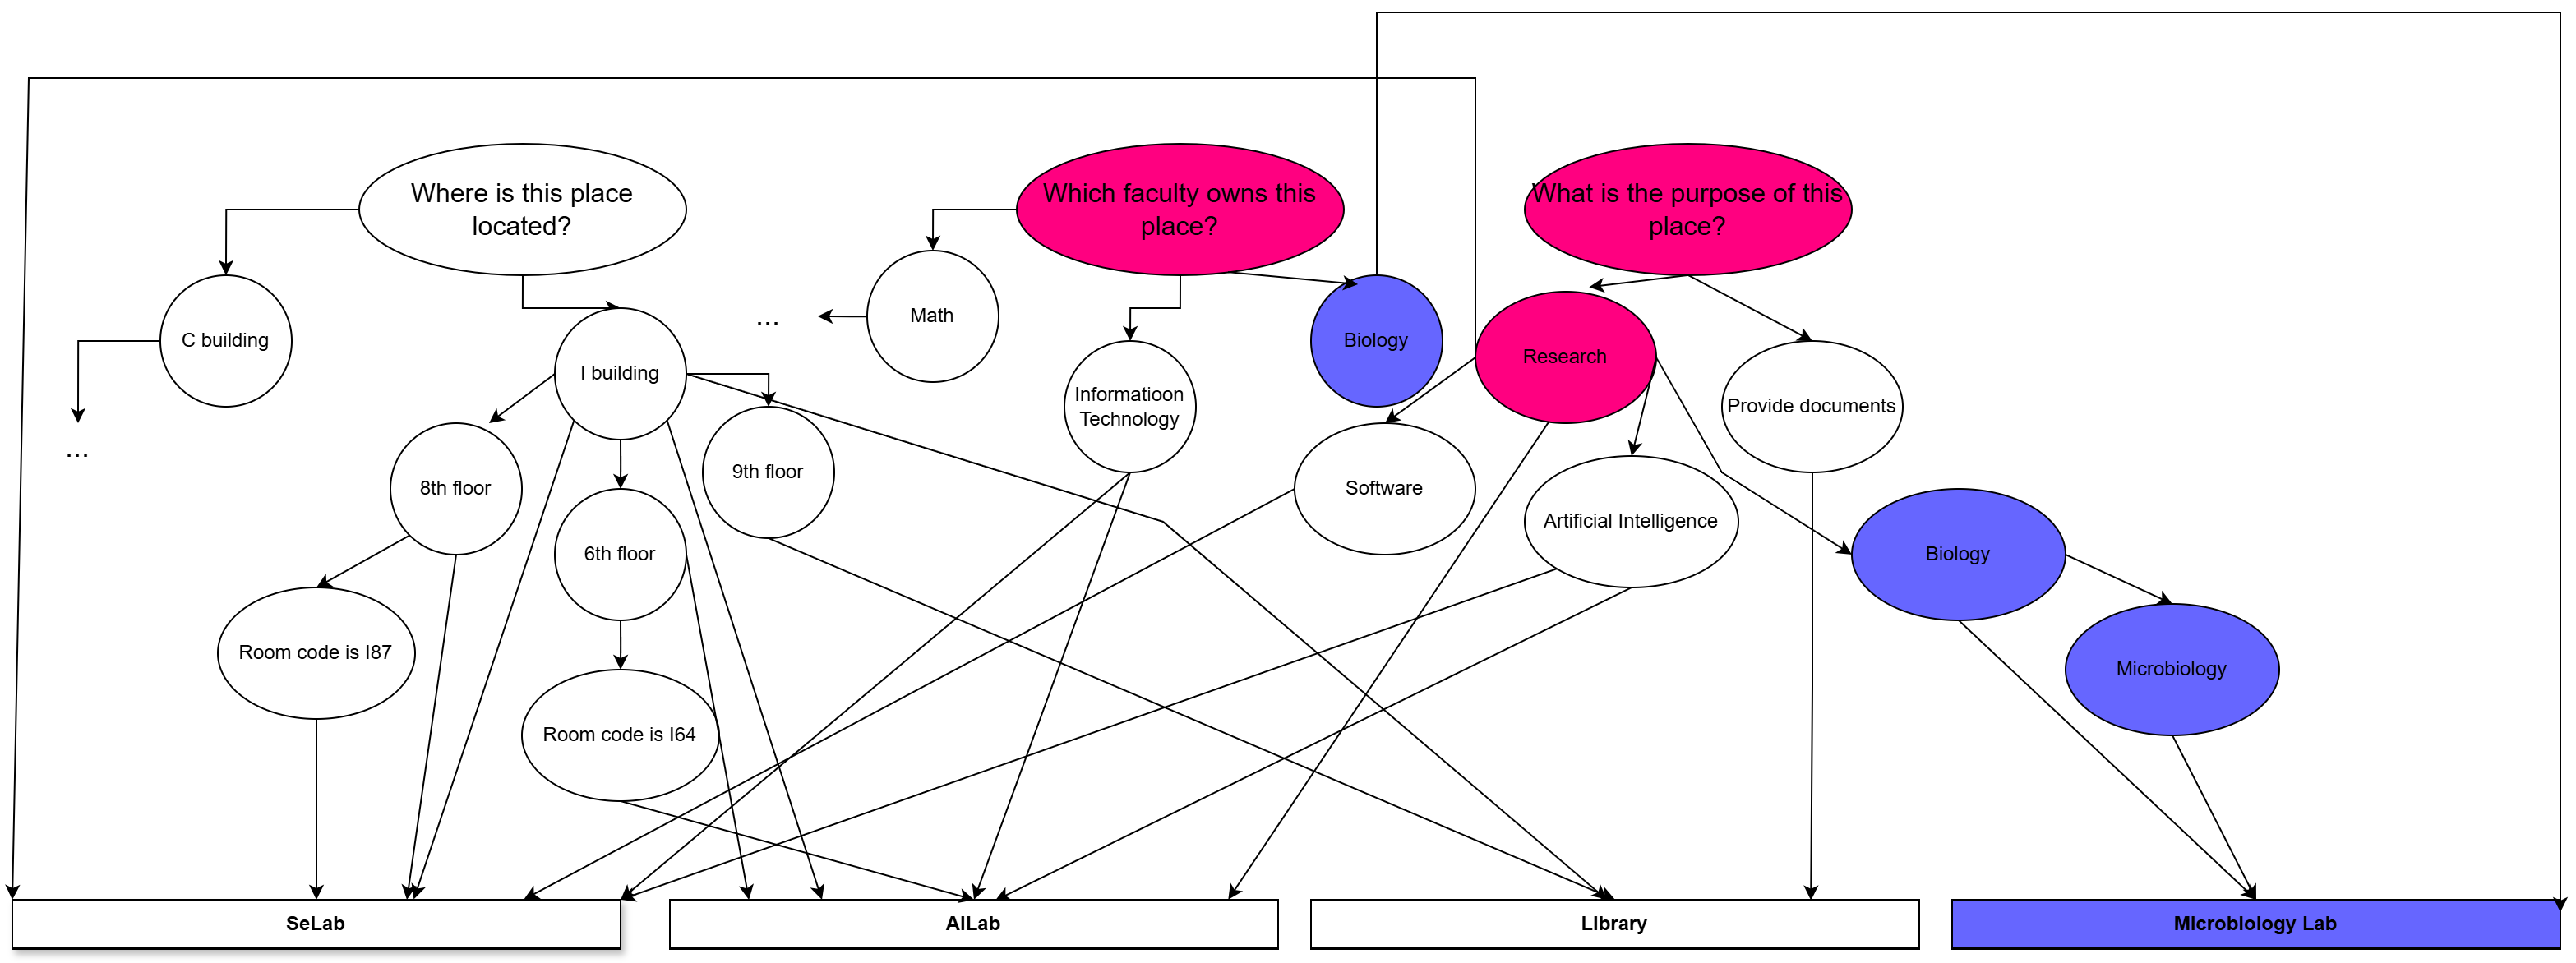
\includegraphics[scale=0.15]{content/resources/images/chap-problems-solutions/data-management-9.png}
  \caption{The hierarchy being updated with \texttt{Microbiology Lab}.}
  \label{fig:data-management-9}
\end{figure}

\subsubsubsubsection*{Add a new rule}\label{subsubsubsub:rules}
With each attribute on a different \texttt{SUB\_ROOT}, users can manually define new rules that can be considered when querying. The process of adding a new rule can also be done automatically, as follows:
\begin{lstlisting}[style=cSharp]
public async Task AddRule(string rule) {
    OpenAI openAI = new OpenAI();
    Helper helper = new Helper();
    foreach (int sub_root in nodes[root].children) {
        string response = await openAI.OpenAIGetAnswer("\nRule: " + rule + "\nQuestion: " + nodes[sub_root].data, 
@"Please answer if the following rule serves as extra information for defining the structure of the answer for the following question.
Return exactly 'YES' if the query answer the question, 'NO' otherwise.
NO OTHER WORDS
");
        response = helper.refineResponse(response);
        if (response.Contains("YES")) {
            nodes[sub_root].rules.Add(rule);
        }
    }
}
\end{lstlisting}

The users only need to define a new rule, the rule is then matched to the appropriate \texttt{SUB\_ROOT}.

\begin{figure}[ht]
  \centering
  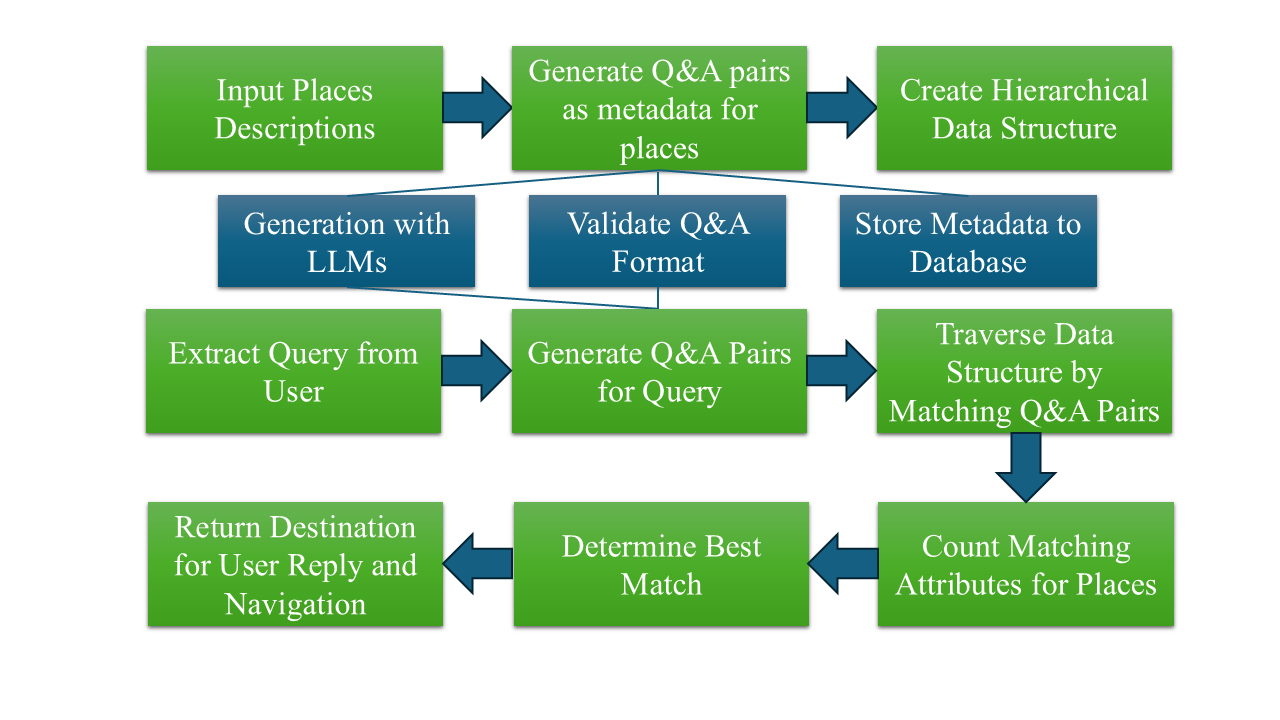
\includegraphics[scale=0.5]{content/resources/images/chap-problems-solutions/data-management-0.png}
  \caption{LLM-Driven Hierarchical Database: Construction and Query Processing Workflow.}
  \label{fig:data-management-0}
\end{figure}

\chapter{ANNOTATION SYSTEM FOR MEDICAL DATA WITH SMART ASSISTANCE}
\label{sec:ANNOTATION SYSTEM FOR MEDICAL DATA WITH SMART ASSISTANCE}
\begin{ChapAbstract}
Chapter 4 details the design, implementation, and evaluation of an integrated AI assistant for smart navigation. This chapter presents a comprehensive system architecture that unifies multiple components: a data generation module, a cloud-based Firebase database with a hierarchical data structure, and an AI assistant powered by a state-of-the-art large language model (LLM) for natural language processing. It further explains the development of AI navigation capabilities using the Vuforia Engine and Creator App to enable real-time augmented reality experiences. The chapter also describes the user interface design—including an interactive home screen, AR navigation overlays, and a dedicated Q\&A metadata generation application—ensuring a seamless and intuitive user experience. A detailed demo plan is provided to illustrate the system's performance in diverse indoor environments.
\end{ChapAbstract}

\section{System Architecture}
This section presents an overview of the platform's system architecture, which is designed to be modular, scalable, and responsive for data annotation workflows. Figure~\ref{fig:system-architecture} illustrates the interconnected components that form the platform's ecosystem, comprising a client-side web application, a cloud-hosted serverless backend, and integrations with specialized external services.

\begin{figure}[ht]
\centering
\includegraphics[width=0.9\textwidth]{content/resources/architecture.png} % Placeholder for diagram
\caption{Overall System Architecture.}
\label{fig:system-architecture}
\end{figure}

\subsection{Client-Side Application}
The client-side application provides the user interface for interacting with the platform. It runs within a standard web browser and is responsible for data presentation, user input, and real-time visualization of workflows and annotations.

\subsubsection{Web Browser Interface}
Users access the platform through a modern web browser. A dedicated Nginx reverse proxy manages traffic routing, serving the frontend assets and securely proxying specific requests to external services where necessary.

\subsubsection{Frontend Technologies}
The user interface is built as a React application, utilizing the \texttt{Refine.dev} framework to streamline development of CRUD operations and application logic. Visual consistency is provided by \texttt{Ant Design} components. For workflow design, the platform integrates \texttt{XYFlow} to enable interactive graphical editing of workflow graphs. Additionally, the \texttt{OHIF Viewer} is embedded for specialized medical imaging annotation and viewing functionalities.

\subsection{Backend Services (Supabase)}
The backend operates on a serverless architecture, leveraging Supabase to provide core database, authentication, and real-time capabilities.

\subsubsection{Supabase Ecosystem}
The entire backend resides within the Supabase platform, which provides a comprehensive suite of cloud-hosted services. This includes a robust \texttt{PostgreSQL Database} for all data storage, \texttt{Supabase Auth} for user authentication and authorization, and \texttt{Supabase Realtime} for instant data synchronization to connected clients.

\subsubsection{Data Storage and Logic}
All persistent data and core business logic are managed within the PostgreSQL database. This includes structured data for projects, tasks, and users, along with JSONB fields for flexible workflow stage configurations. Complex operations and state transitions are encapsulated within \texttt{SQL Functions}, which serve as the primary executable logic, while \texttt{SQL Views} provide abstracted and secure data access layers for the frontend.

\subsection{External Integrations}
The platform extends its capabilities through seamless integration with specialized external systems, particularly relevant for advanced medical imaging and AI-assisted annotation.

\subsubsection{Specialized Tools}
For AI-assisted medical image labeling, the platform integrates with the \texttt{MONAI Label App}, a server-side framework that offers machine learning model inference. Additionally, \texttt{Orthanc}, a lightweight DICOM server, functions as a primary source for medical image data, providing seamless access to studies for annotation tasks.
Generated latex
\section{System Requirements}

This section outlines the hardware and software prerequisites for deploying and utilizing the data annotation platform. The system is designed as a web-based application, with a distinct client-side interface and a cloud-hosted backend.

\subsection{Client-Side Requirements}
This section details the prerequisites for end-users interacting with the platform's web-based frontend.

\subsubsection{Software Requirements}
\begin{itemize}
    \item \textbf{Web Browser:} A modern web browser (e.g., Google Chrome, Mozilla Firefox, Microsoft Edge, Apple Safari) is required. The browser must support contemporary web standards, including JavaScript and CSS, for proper rendering and interactive functionality of the React-based frontend developed with Refine.dev and Ant Design.
    \item \textbf{Internet Connectivity:} A stable and reliable internet connection is essential for users to access the platform's cloud-hosted backend, retrieve project data, submit annotations, and receive real-time updates through Supabase's real-time capabilities.
\end{itemize}

\subsubsection{Hardware Recommendations}
\begin{itemize}
    \item \textbf{Device Type:} A desktop or laptop computer is recommended for optimal user experience. This allows for a larger screen area and precise input methods, which are beneficial for detailed annotation tasks and complex workflow graph design.
    \item \textbf{Processing Power \& Memory:} Devices should possess sufficient computing resources, typically 8GB of RAM or more and a modern multi-core CPU, to ensure smooth operation of demanding web applications, efficient rendering of intricate user interface components, and responsive interaction with large datasets that may be displayed in the browser.
    \item \textbf{Display Resolution:} A minimum screen resolution of 1920x1080 pixels is advisable. This ensures that all components of the user interface, particularly the interactive workflow editor and the integrated annotation tools, are displayed comprehensively without excessive scrolling or scaling.
\end{itemize}

\subsection{Server-Side Requirements}
This section outlines the infrastructure and software prerequisites for hosting and operating the platform's backend services and database.

\subsubsection{Supabase Backend Infrastructure}
The platform's backend is fundamentally architected around the \textbf{Supabase} ecosystem. This choice simplifies deployment and management by providing an integrated suite of services:
\begin{itemize}
    \item \textbf{PostgreSQL Database:} As the core data store, a PostgreSQL instance (version 12 or later recommended) is required. Supabase natively provides this, offering robust support for concurrent connections, efficient handling of JSONB data types for flexible configurations, and the execution of custom PL/pgSQL functions that encapsulate all backend business logic and workflow automation. Adequate and scalable disk space within the PostgreSQL environment is necessary to accommodate project data, tasks, annotations, and the comprehensive audit trail.
    \item \textbf{Integrated Services:} Supabase natively includes \textbf{Supabase Auth} for robust user authentication and authorization, and \textbf{Supabase Realtime} for real-time data synchronization.
    \item \textbf{System Automation:} The platform's automated workflow orchestration relies heavily on scheduled PostgreSQL functions acting as cron jobs. Supabase's architecture inherently supports the reliable execution of these functions at regular intervals, which is critical for triggering automated tasks assigned to virtual users and ensuring continuous workflow progression.
\end{itemize}
As an open-source platform, Supabase can be deployed as a managed cloud service or self-hosted, including via Docker container images, offering flexibility in infrastructure provisioning.

\subsubsection{External System Integrations}
The platform's comprehensive functionality is significantly enhanced through its ability to integrate with specialized external systems.
\begin{itemize}
    \item \textbf{Medical Imaging Archives (e.g., Orthanc):} For projects involving medical imaging data, network connectivity and appropriate API access permissions are required to integrate with external PACS (Picture Archiving and Communication System) or VNA (Vendor Neutral Archive) systems, such as Orthanc, for importing data items.
    \item \textbf{Annotation Toolkits (e.g., OHIF Viewer, MONAI):} While these are typically client-side components or frameworks leveraged for specific annotation tasks, the backend may require configured endpoints or data exchange protocols to seamlessly interact with instances of OHIF Viewer or MONAI, whether they are hosted externally or bundled within the client environment.
    \item \textbf{Machine Learning Models:} For advanced features like Model-Assisted Labeling (MITL), the backend requires stable network access to external machine learning model API endpoints. This includes consistent connectivity and valid API keys or authentication credentials to securely invoke these services for inference or prediction.
\end{itemize}

\subsubsection{Security \& Permissions}
\begin{itemize}
    \item \textbf{API Keys and Credentials Management:} Secure storage and management of API keys, access tokens, and other credentials for Supabase, external machine learning models, and any integrated third-party data sources (e.g., Orthanc) are paramount to maintaining system security.
    \item \textbf{Network Configuration:} Appropriate firewall rules and network security policies must be implemented on the server infrastructure to allow only necessary inbound and outbound connections for the backend services and external integrations, while strictly adhering to a strong security posture.
\end{itemize}

Here's the updated LaTeX code, with the figures integrated and captions updated. I've used X.Y as placeholders for chapter and figure numbers, as requested, and made sure the image paths are correct.

Generated latex
\section{Platform Features}
This section provides a comprehensive overview of the data annotation platform's features, highlighting its core functionalities, architectural design principles, and collaborative capabilities. The design emphasizes modularity, scalability, and an intuitive user experience, while leveraging a robust backend for automated processes.

\subsection{Authorization and Access Control}
The platform incorporates a sophisticated authorization system designed for granular control over resources and actions, ensuring data security and user privacy.

\subsubsection{Attribute-Based Access Control (ABAC)}
Instead of rigid, static roles, the system employs Attribute-Based Access Control (ABAC). Permissions are dynamically evaluated based on various attributes, including those of the user (e.g., role within a project), the resource (e.g., project, task, assignment), and the specific action being attempted (e.g., `create`, `delete`, `comment`). This enables highly flexible and fine-grained security policies.

\subsubsection{Contextual and Secure Authentication}
Access decisions are inherently contextual, with user permissions determined by their specific role within a given project. User authentication is securely managed through Supabase Auth, and user profiles store additional attributes (e.g., full name, avatar) that can further inform access control policies.

\begin{figure}[h!]
    \centering
    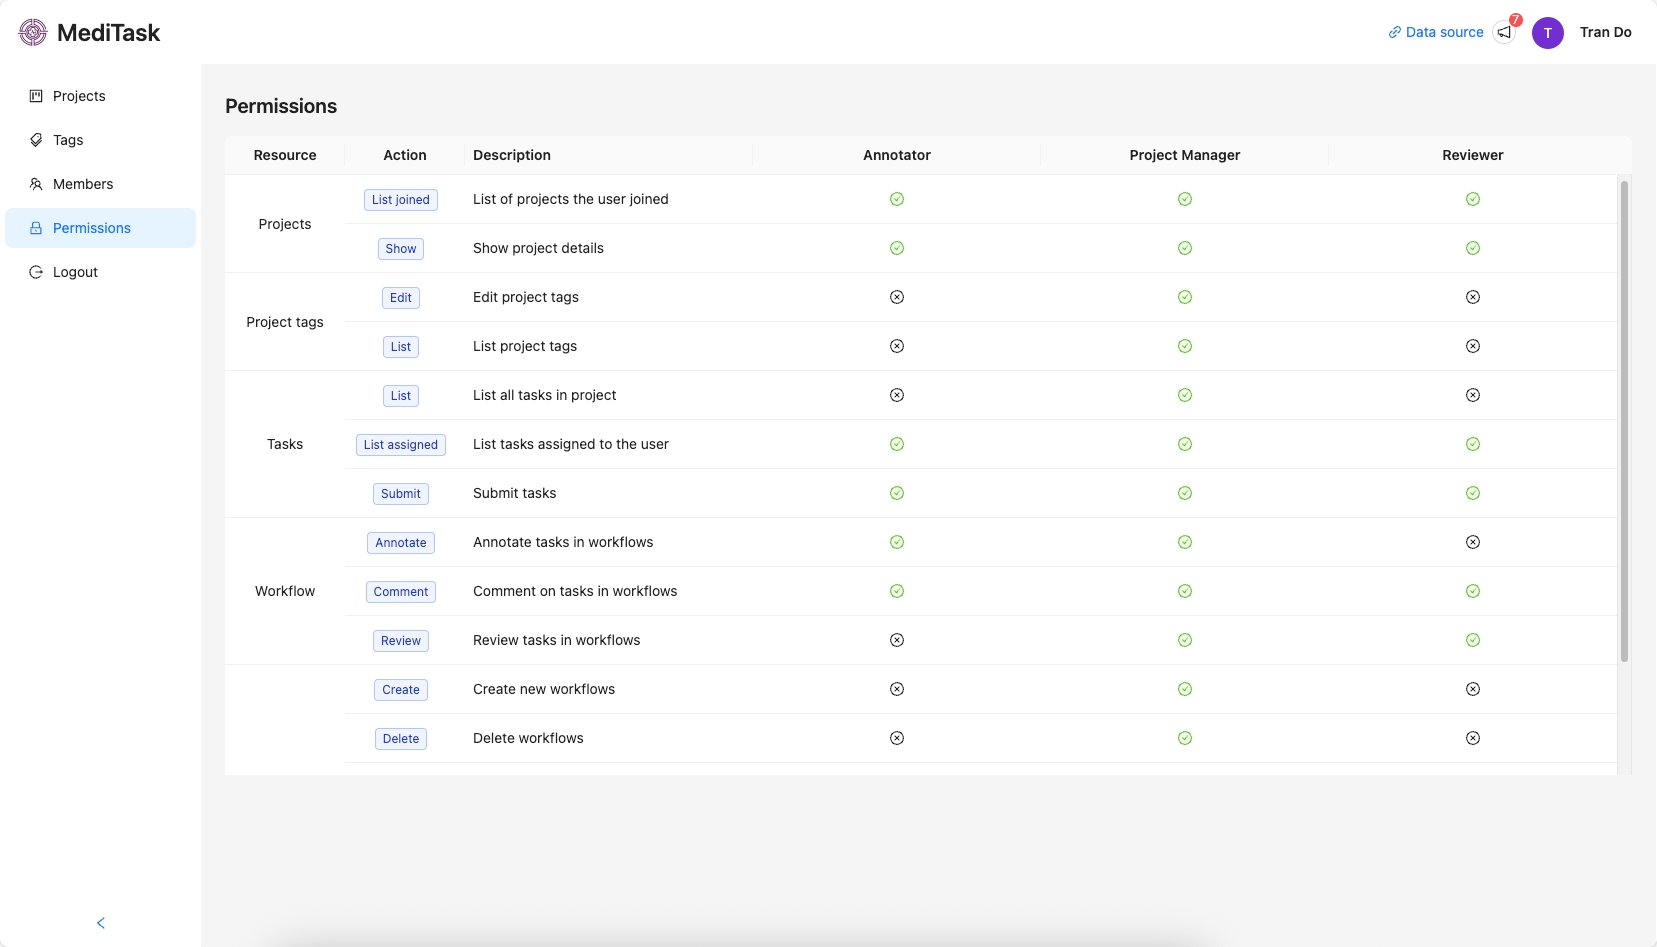
\includegraphics[width=1\textwidth]{content//resources//features//permissions.png}
    \caption{Granular Permissions Configuration Interface}
    \label{fig:permissions-config}
\end{figure}

\subsection{Workflow Management}
At the heart of the platform lies a powerful and adaptable workflow engine that facilitates the construction and execution of complex data processing pipelines.

\subsubsection{Dynamic Workflow Graphs}
Workflows are visually represented and defined as directed graphs, comprising interconnected stages (nodes) and connections (edges). This graph structure is customizable per project, allowing for bespoke data processing flows. Figure~\ref{fig:workflow-editor-simple} illustrates the intuitive drag-and-drop interface for designing workflows, while Figure~\ref{fig:workflow-editor-advanced} demonstrates a more complex workflow incorporating routing and consensus stages.

\begin{figure}[h!]
    \centering
    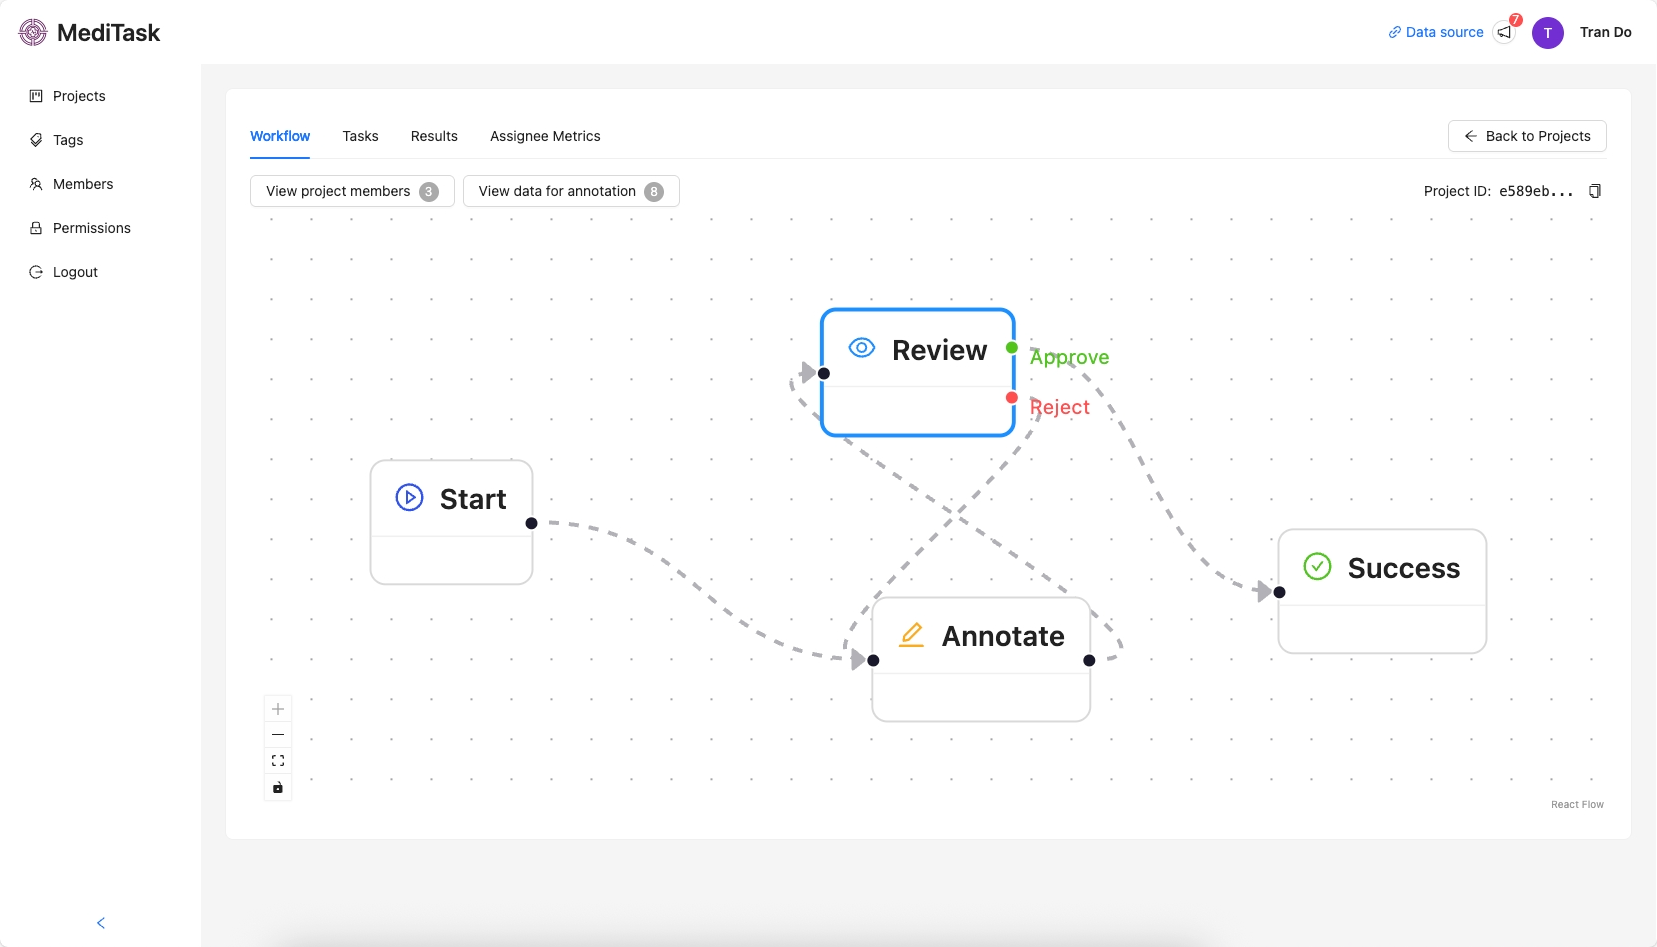
\includegraphics[width=1\textwidth]{content/resources/features/simple workflow.png}
    \caption{Workflow Design Interface}
    \label{fig:workflow-editor-simple}
\end{figure}

\begin{figure}[h!]
    \centering
    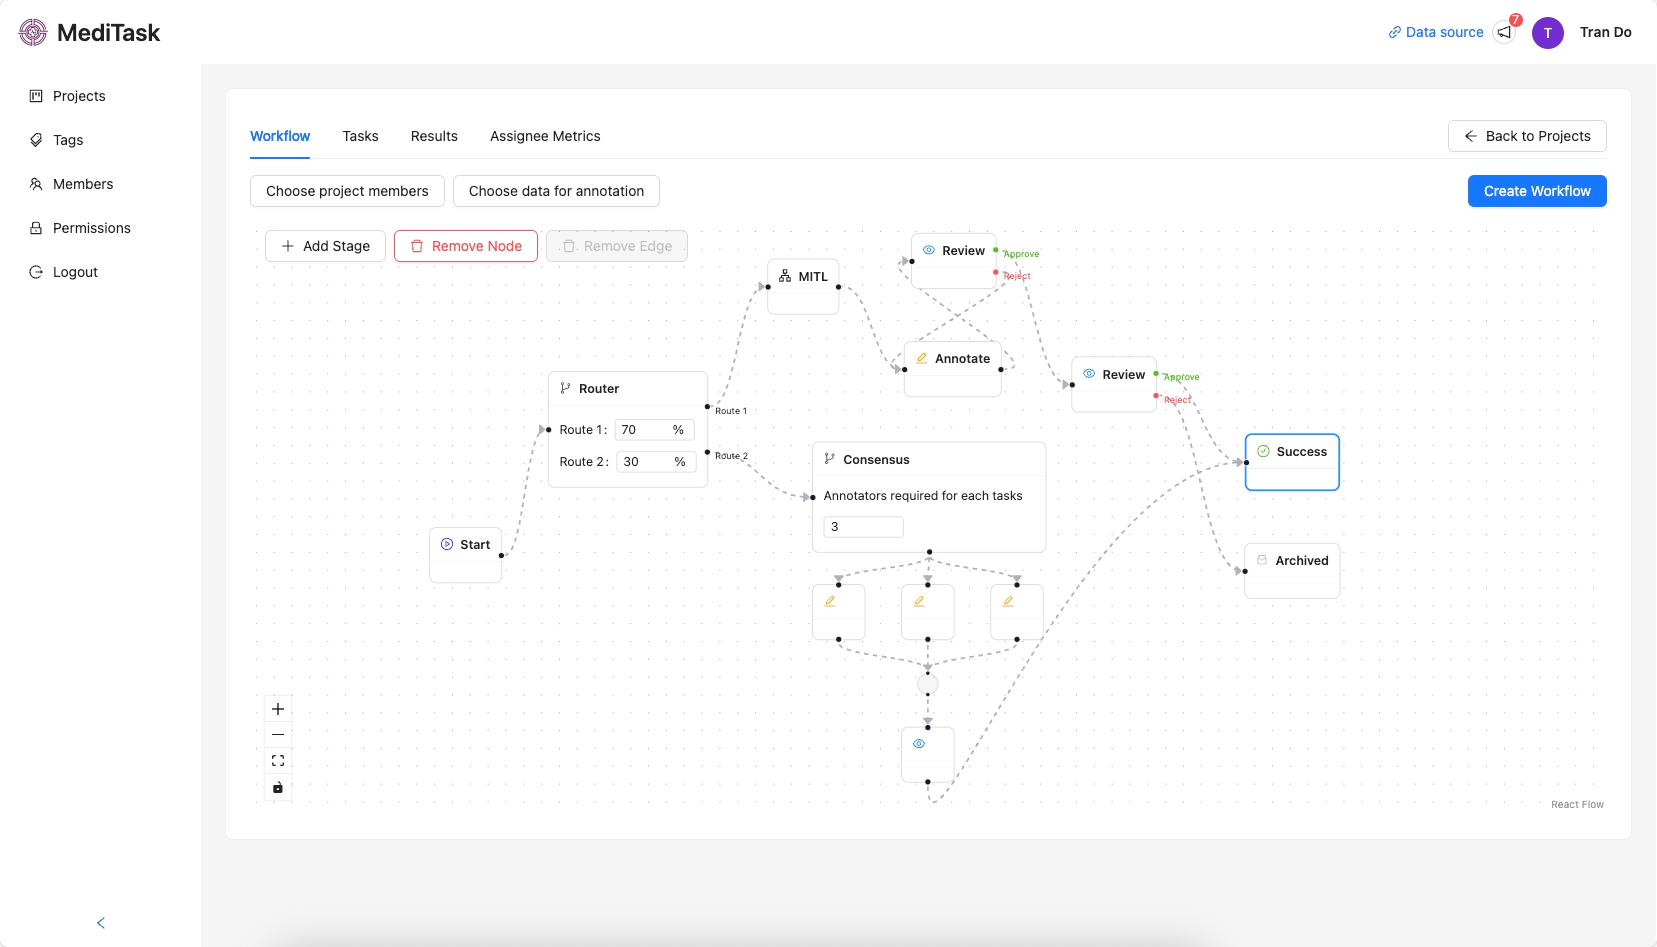
\includegraphics[width=1\textwidth]{content/resources/features/complex workflow.png}
    \caption{Advanced Workflow with Router and Consensus Stages}
    \label{fig:workflow-editor-advanced}
\end{figure}

\subsubsection{Customizable Stages and Conditional Logic}
Each workflow stage possesses a distinct type (e.g., \texttt{ANNOTATE}, \texttt{REVIEW}, \texttt{CONSENSUS}) and can host unique custom configurations. The system supports advanced conditional branching, enabling distinct success and failure paths for tasks at each stage, ensuring resilient workflow progression. As shown in Figure~\ref{fig:workflow-select-members}, users can easily select project members and their roles, which can then be assigned to workflow stages.

\begin{figure}[h!]
    \centering
    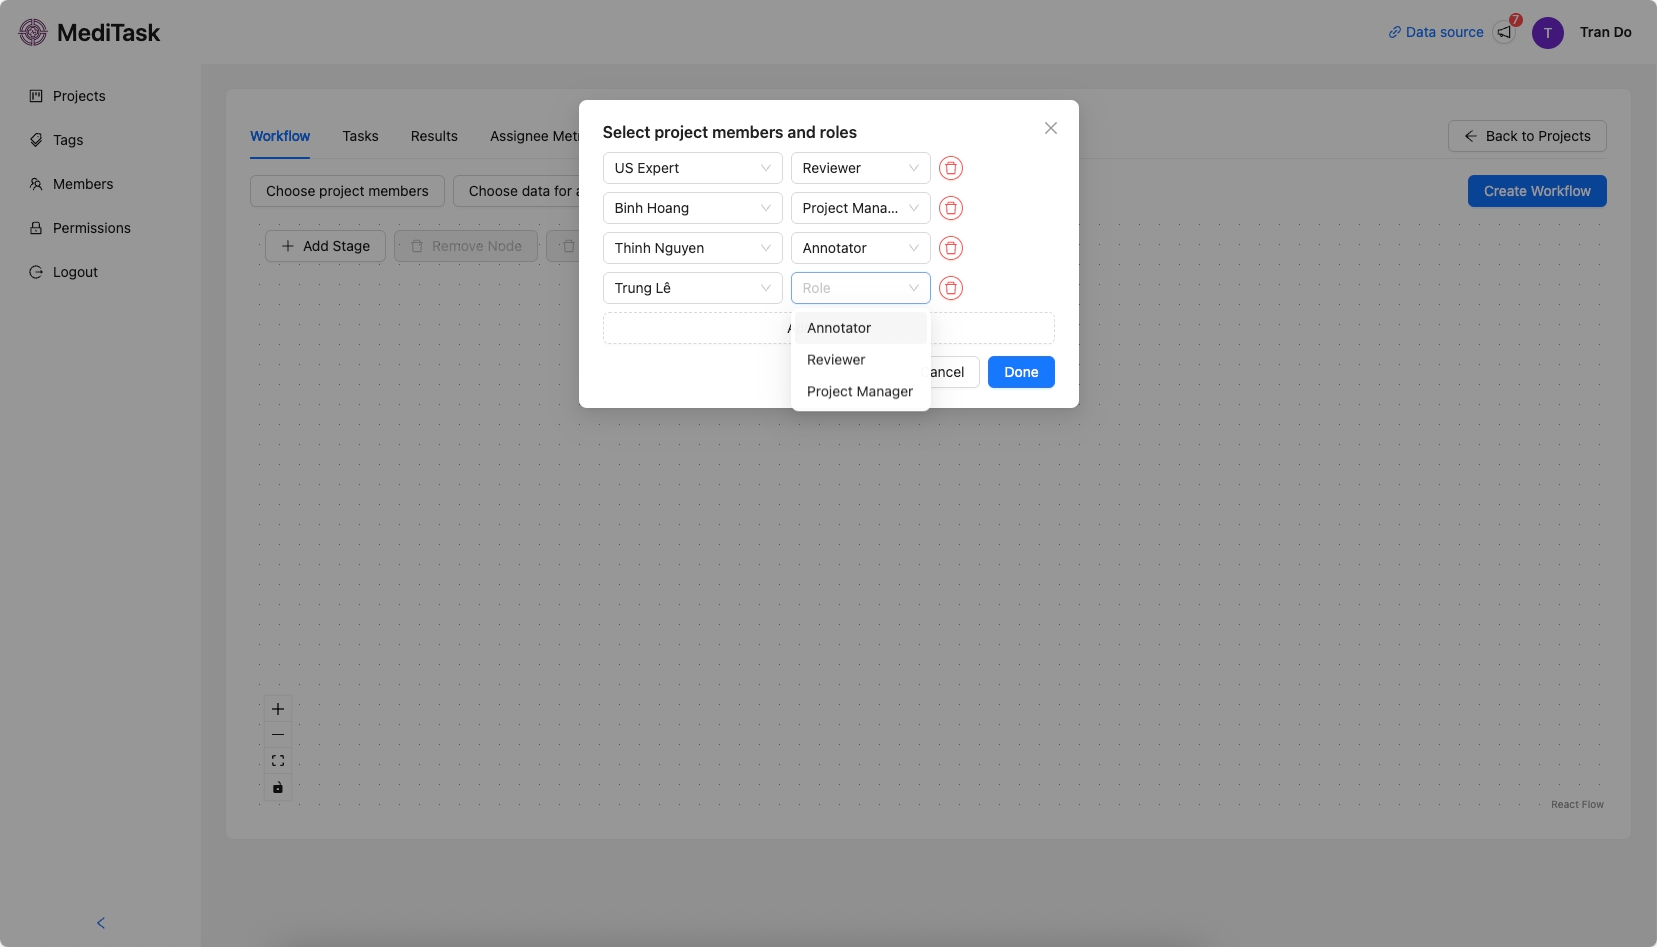
\includegraphics[width=0.6\textwidth]{content/resources/features/choose members.png}
    \caption{Selecting Project Members for Workflow Assignment}
    \label{fig:workflow-select-members}
\end{figure}

\subsubsection{Automated Assignee Selection}
The platform can automatically determine the subsequent assignee for a task based on functions linked to each workflow stage. This capability underpins complex routing logic, optimizing task distribution and flow. Figure~\ref{fig:workflow-select-data} demonstrates the process of selecting specific data instances to be included in a workflow, ensuring only relevant data undergoes the defined process.

\begin{figure}[h!]
    \centering
    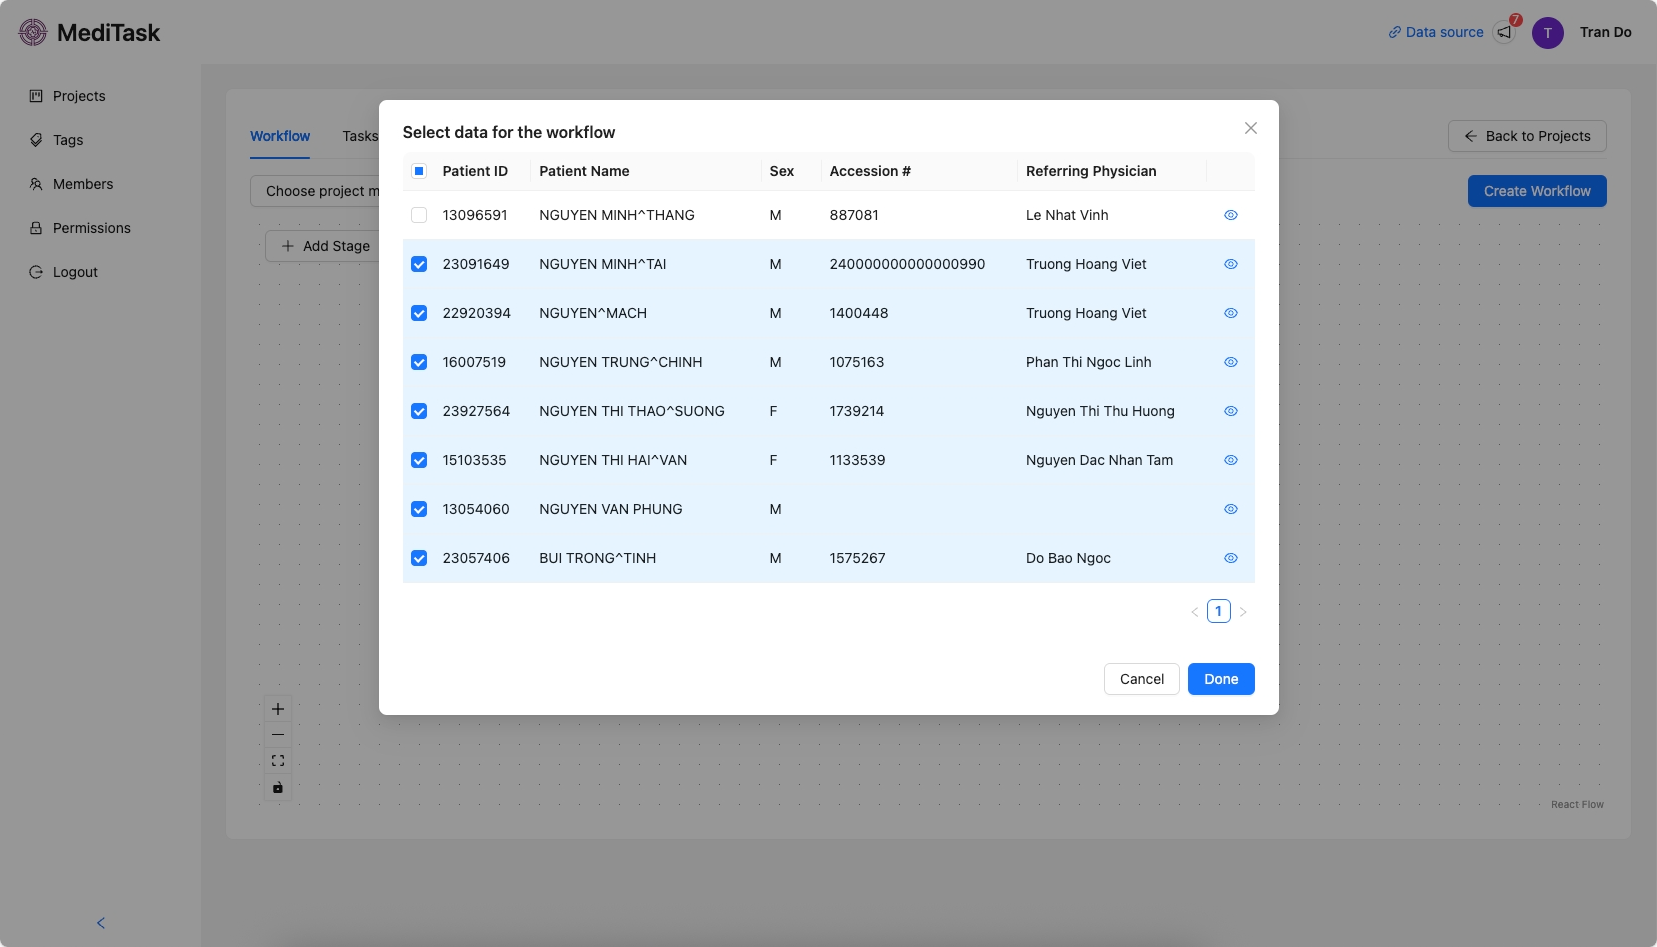
\includegraphics[width=0.6\textwidth]{content/resources/features/choose dataset.png}
    \caption{Selecting Data Instances for Workflow Processing}
    \label{fig:workflow-select-data}
\end{figure}

\subsection{Project \& Task Management}
Comprehensive tools are provided for the organization and management of projects and their constituent tasks.

\subsubsection{Centralized Project Hub}
Projects serve as the primary organizational unit, encapsulating datasets, tasks, and member assignments. Each project is defined by a name, description, and an associated set of members, providing a consolidated view for all related activities. Figure~\ref{fig:project-list} illustrates the centralized project hub, allowing users to overview and manage their ongoing annotation efforts. Projects can also be categorized using a flexible, color-coded tagging system, enhancing visual identification and search capabilities, as seen in Figure~\ref{fig:tags-list}.

\begin{figure}[h!]
    \centering
    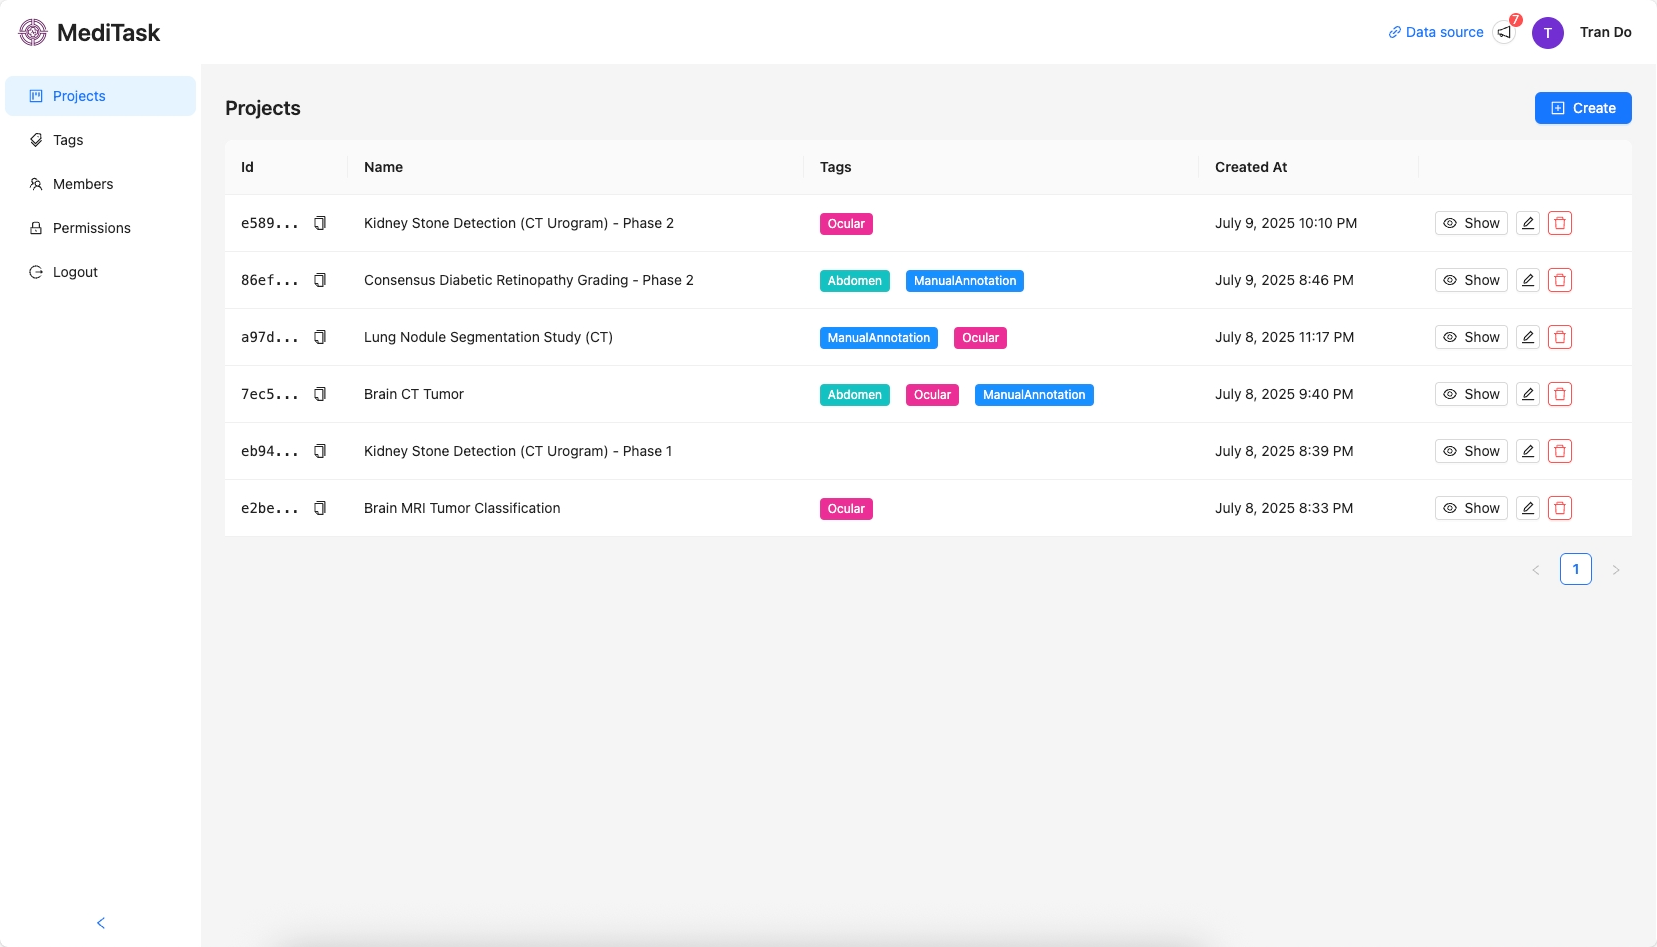
\includegraphics[width=1\textwidth]{content//resources//features//projects.png}
    \caption{Layout of Project Management Page}
    \label{fig:project-list}
\end{figure}

\begin{figure}[h!]
    \centering
    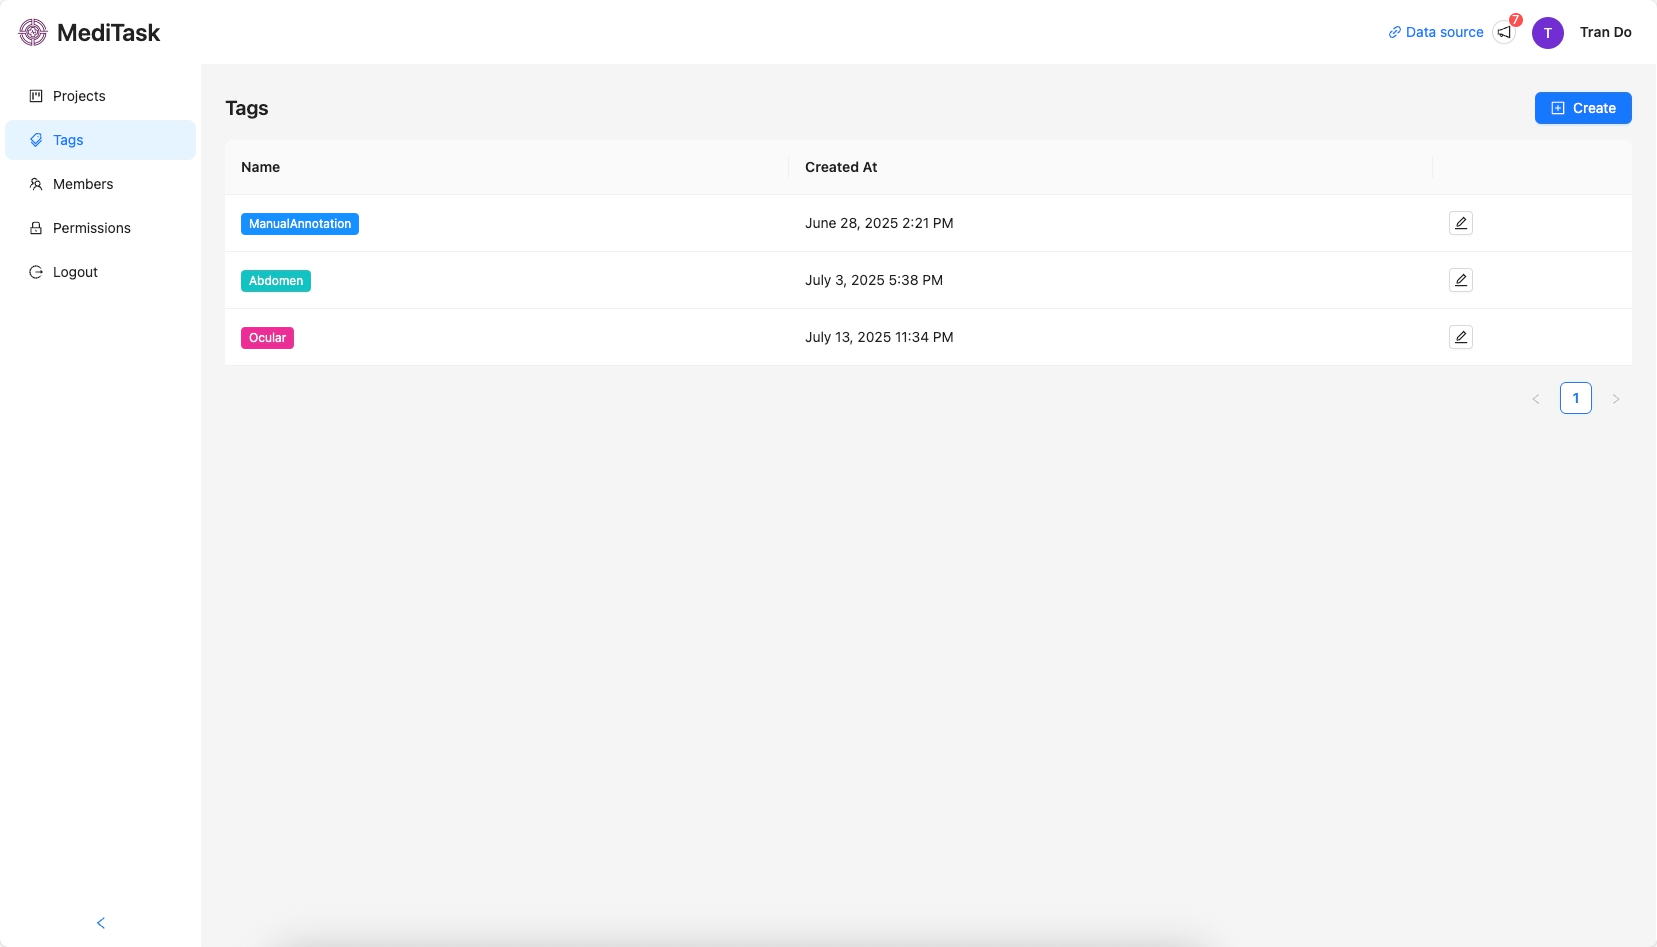
\includegraphics[width=1\textwidth]{content//resources//features//tags.png}
    \caption{Project Tag Management Interface}
    \label{fig:tags-list}
\end{figure}

\subsubsection{Task Lifecycle Management}
Tasks represent discrete units of work tied to specific data items. They transition through various statuses (e.g., \texttt{PENDING}, \texttt{COMPLETED}) as they advance through the defined workflow, ensuring clear visibility of progress. Figure~\ref{fig:tags-list} and Figure~\ref{fig:tasks-tab-1} showcase different views of the task list within a project, providing comprehensive oversight of task status, assignment, and progress.

\begin{figure}[h!]
    \centering
    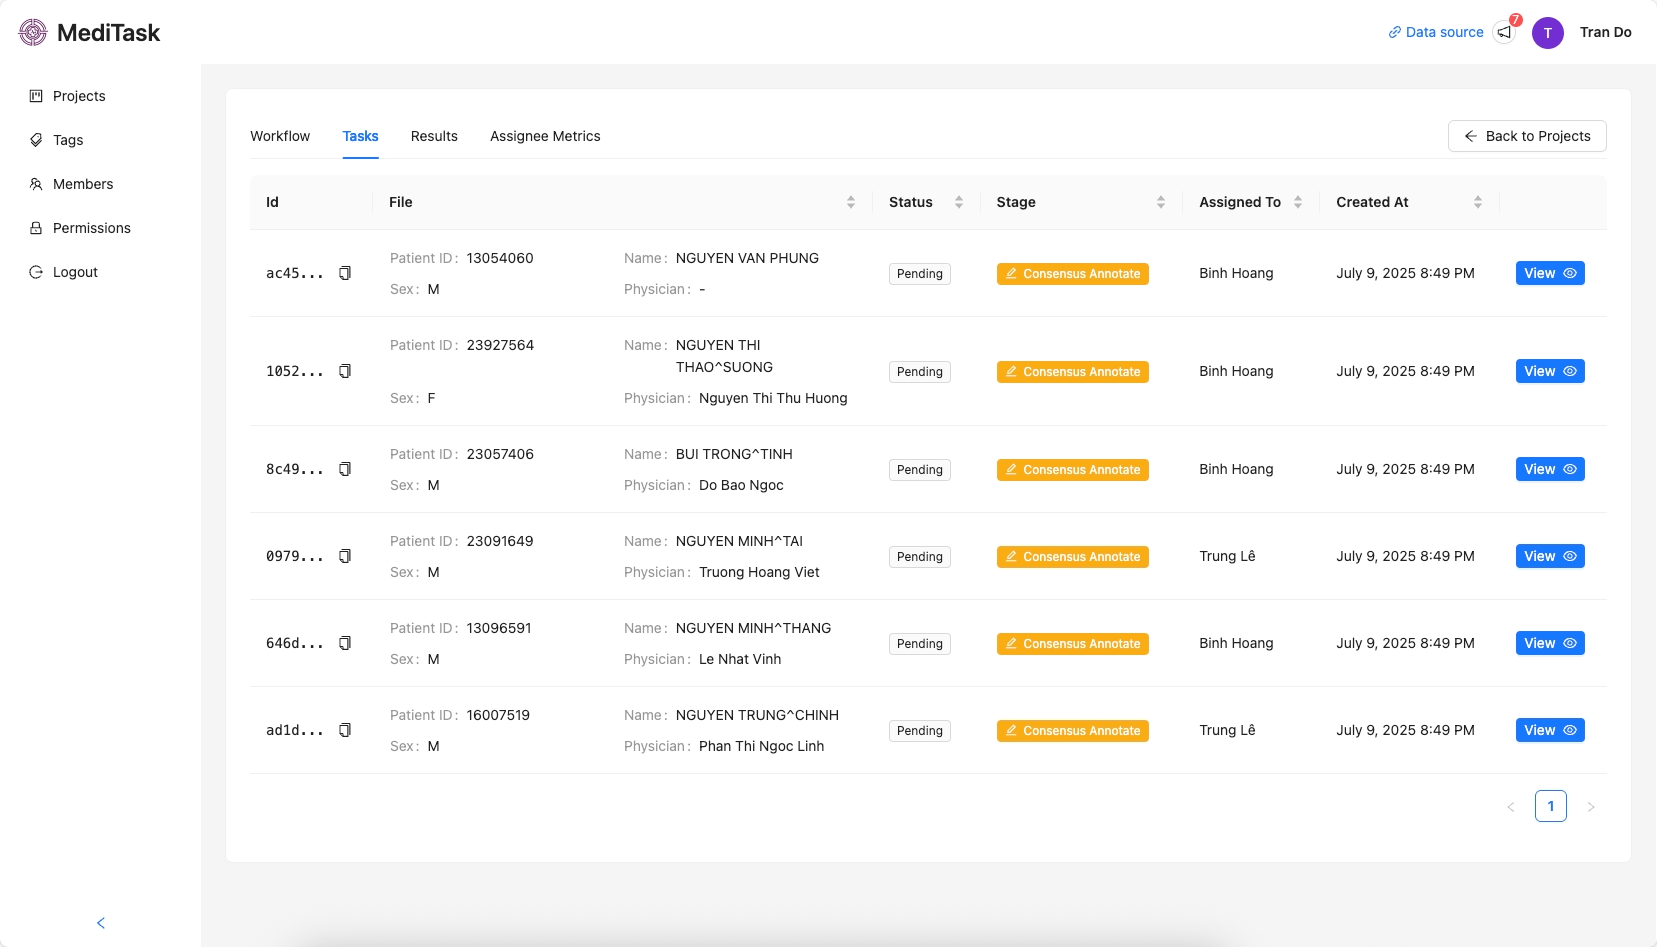
\includegraphics[width=1\textwidth]{content/resources/features/tasks.png}
    \caption{Task List View within a Project}
    \label{fig:tasks-tab-1}
\end{figure}

\subsubsection{Detailed Task Assignments}
Task progression through a workflow is managed via assignments. Each assignment links a task to a specific user at a particular workflow stage, meticulously tracking its status, start time, and completion time, creating an auditable trail.

\subsection{Member Management}
The platform facilitates the effective management of users and their roles within projects.

\subsubsection{User and Project-Level Role Management}
Administrators can create, list, and modify user accounts within the system. Critically, roles are assigned on a per-project basis, allowing for granular control over user permissions and responsibilities tailored to each project's needs. While a dedicated member list view is not shown, the `Permissions` interface (Figure~\ref{fig:permissions-config}) implicitly demonstrates the role-based access control for different user types.

\subsection{Annotation \& Collaboration}
The platform is meticulously designed to foster efficient and accurate data annotation through a robust collaborative environment.

\subsubsection{Integrated Annotation Tools}
The system seamlessly integrates with industry-standard tools such as OHIF Viewer, MONAI, and Orthanc. This integration supports advanced medical imaging annotation workflows and enables AI-assisted labeling functionalities. Figure~\ref{fig:annotation-viewer} provides a view of the integrated medical imaging annotation environment, while Figure~\ref{fig:orthanc-integration} shows the external Orthanc integration for data source management.

\begin{figure}[h!]
    \centering
    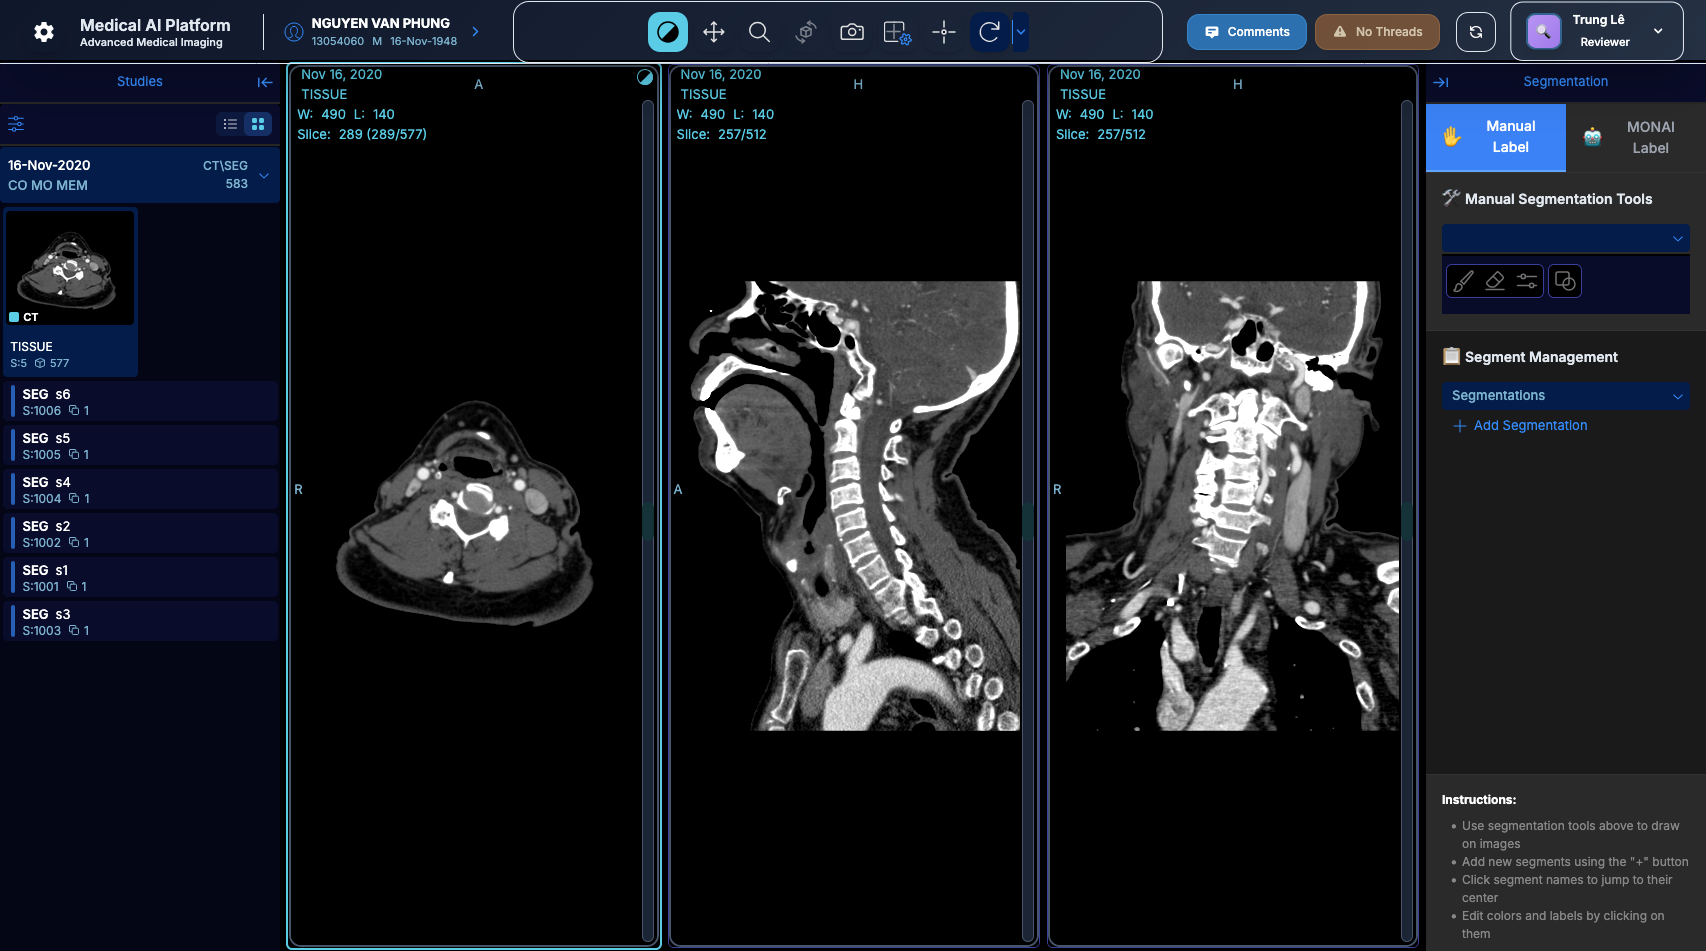
\includegraphics[width=1\textwidth]{content/resources/features/ohif.png}
    \caption{Integrated Medical Imaging Annotation Viewer}
    \label{fig:annotation-viewer}
\end{figure}

\subsubsection{Annotation Commenting and Segmentation Data}
Users can leave rich, structured comments on task assignments, facilitating detailed discussions and feedback loops. Figure~\ref{fig:annotation-comments} illustrates the task assessment hub, which includes a dedicated section for comments and collaboration. Tasks are also capable of storing lists of segmentation IDs, which are crucial for image-based annotation tasks involving precise object boundaries.

\begin{figure}[h!]
    \centering
    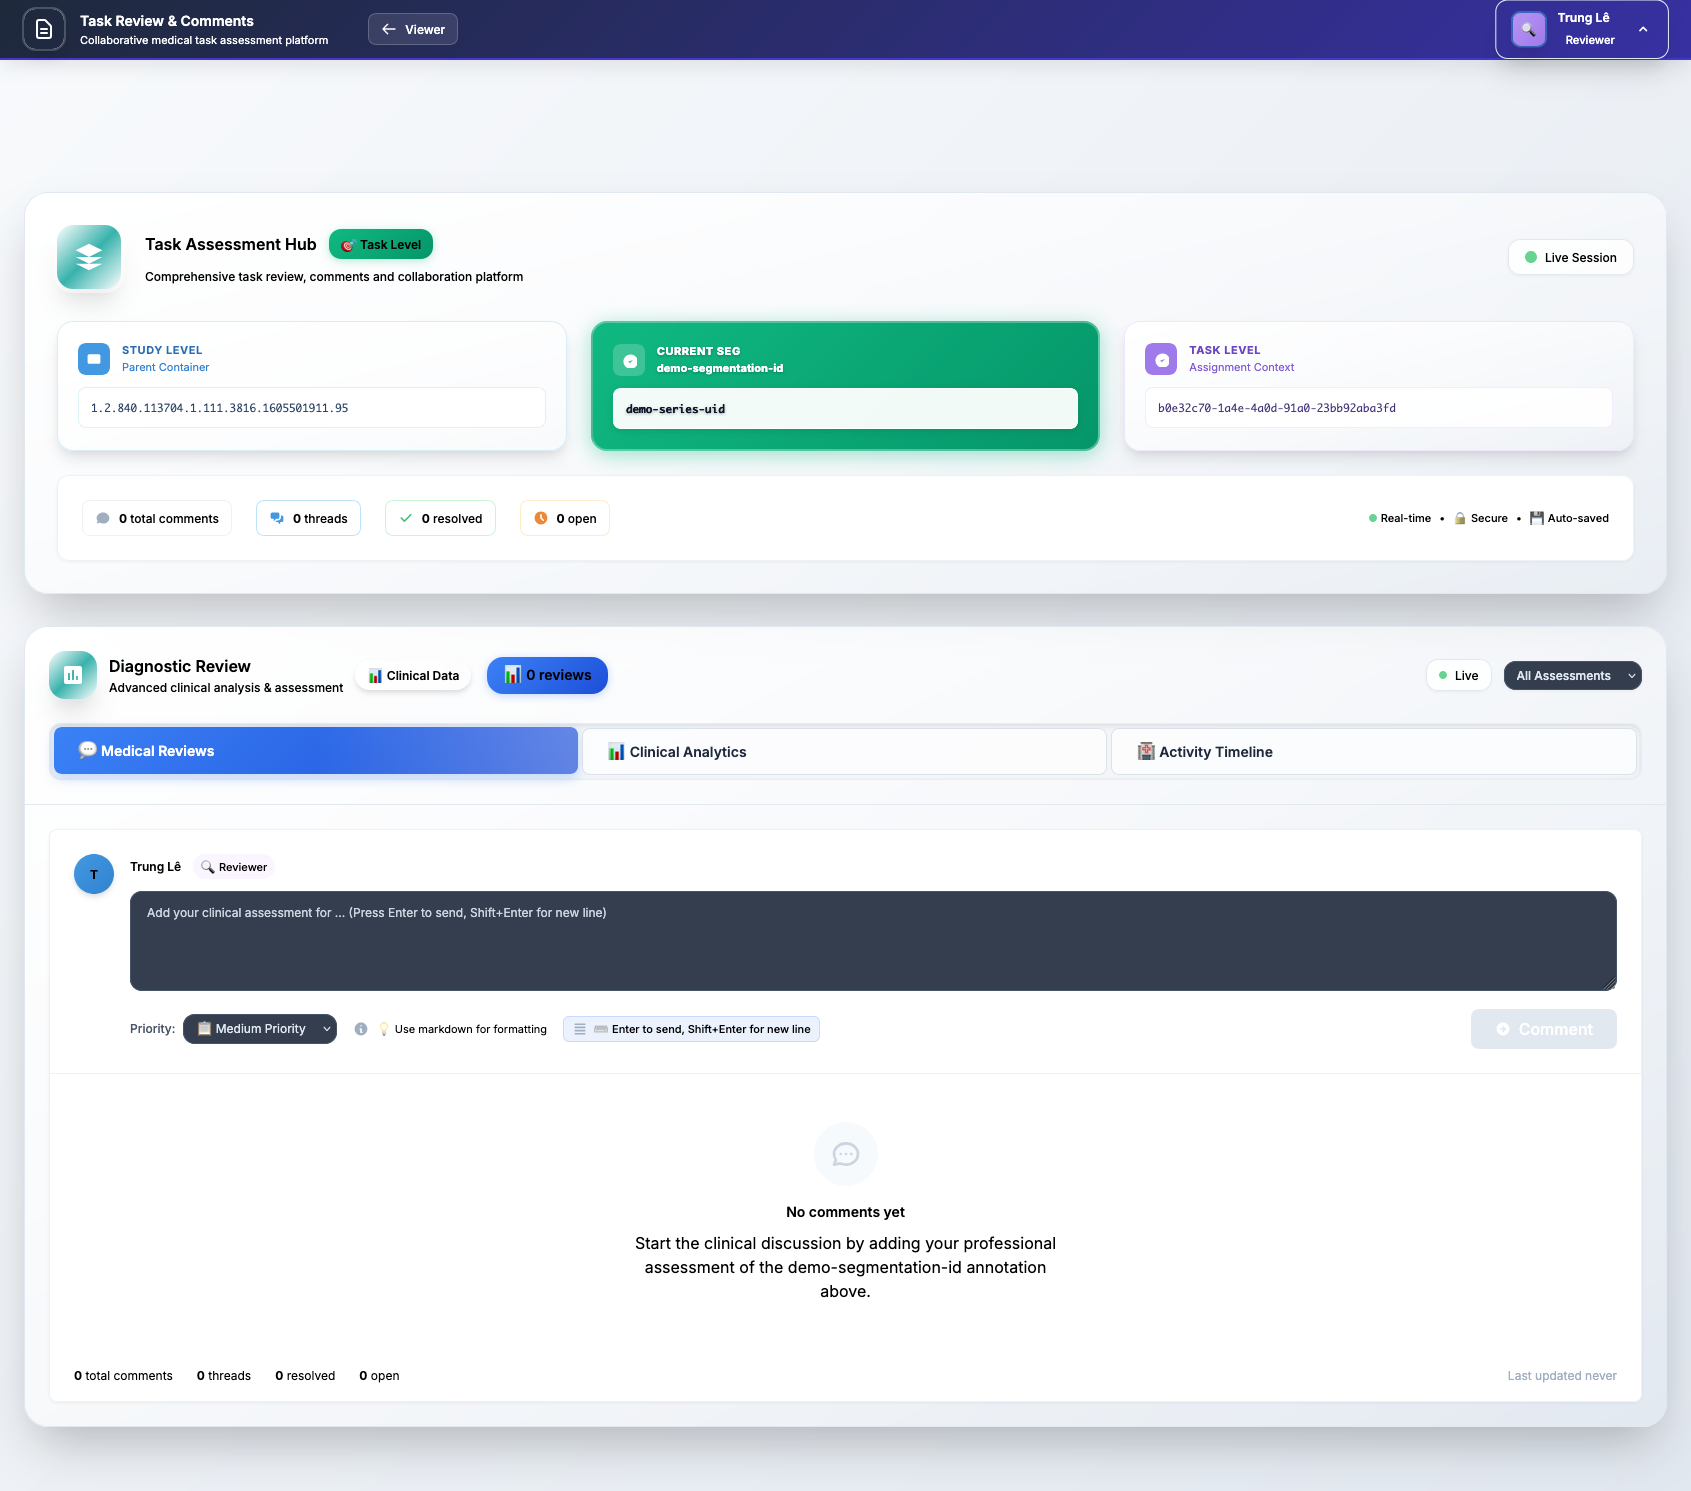
\includegraphics[width=1\textwidth]{content/resources/features/ohif comment.png}
    \caption{Task Assessment Hub with Annotation Commenting}
    \label{fig:annotation-comments}
\end{figure}

\subsubsection{Data Source Integration}
The system can connect to and ingest data items from external sources, including specialized medical imaging archives like Orthanc, streamlining the data acquisition process for annotation.

\begin{figure}[h!]
    \centering
    \includegraphics[width=1\textwidth]{content//resources//features//orthanc.png}
    \caption{Orthanc Data Source Integration Interface}
    \label{fig:orthanc-integration}
\end{figure}

\subsection{Backend Automation: Virtual Users and Cron-Based Workflow Orchestration}
A cornerstone of the platform's backend architecture is its capacity for automated workflow progression, reducing the need for direct human intervention in repetitive or system-driven tasks. This is achieved through a synergy of "virtual users" and scheduled cron jobs, forming an intelligent, SQL-based orchestration layer.

\subsubsection{The Concept of Virtual Users}
To manage automated, non-human operations, the system employs "virtual users." These are specialized user accounts within the `\_users` table, distinguished by an `is\_system` boolean field set to `true`. They act as system-level actors for specific automated functions, such as:
\begin{itemize}
    \item \textbf{START}: Initiates new tasks in a workflow.
    \item \textbf{ROUTER}: Manages conditional logic, directing tasks based on predefined rules embedded in workflow stage configurations.
    \item \textbf{CONSENSUS}: Orchestrates the aggregation and comparison of multiple annotations to determine agreement, critical for quality control.
\end{itemize}
When a task enters a stage requiring automated processing, it is assigned to one of these virtual users within the `\_task\_assignments` table, awaiting system action.

\subsubsection{Cron Jobs: The Automation Trigger}
Unlike human-initiated tasks, tasks assigned to virtual users are processed by scheduled cron jobs. These are PostgreSQL functions configured to execute at regular intervals (e.g., every minute), establishing a robust polling mechanism. Key cron jobs for workflow automation include `workflow\_start`, `workflow\_route`, `workflow\_consensus`, and `workflow\_consensus\_holding`.

\subsubsection{The Automated Orchestration Flow}
The automated workflow progresses through a clear, stateful sequence recorded within the database:
\begin{enumerate}
    \item \textbf{Assignment to Virtual User}: A task transitions to an automated stage (e.g., a `ROUTER` stage), triggering the creation of a new `\_task\_assignments` record that links the task to the stage and the relevant virtual user.
    \item \textbf{Scheduled Execution}: A periodically running cron job (e.g., `workflow\_route()`) is invoked.
    \item \textbf{Task Processing}: The executing function queries `\_task\_assignments` for all 'PENDING' tasks assigned to its corresponding virtual user.
    \item \textbf{Logic Execution}: For each pending task, the function executes specialized logic. For a `ROUTER` stage, this involves interpreting the `custom\_config` JSONB field from the `\_workflow\_stages` entry to determine the next path.
    \item \textbf{Workflow Progression}: Upon logic execution, the function advances the task to the next stage by:
    \begin{itemize}
        \item Updating the current assignment's status to 'COMPLETED'.
        \item Determining the subsequent stage ID using `on\_success\_stage\_id` or `on\_failure\_stage\_id`.
        \item Creating a new `\_task\_assignments` record for the next stage, assigning it to the appropriate human or virtual user. The `previous\_task\_assignment\_id` is linked to the completed assignment, ensuring an immutable and auditable event chain.
    \end{itemize}
\end{enumerate}
This cron-based approach establishes a powerful, asynchronous, and fully automated backend engine, driving the workflow forward in a serverless architecture.

\begin{figure}[h!]
    \centering
    % \includegraphics[width=0.8\textwidth]{path/to/your/workflow\_automation\_flow.png} % No specific image provided for this abstract concept.
    \caption{Conceptual Workflow Automation Flow}
    \label{fig:automation-flow}
\end{figure}

\subsection{Notifications}
A robust, built-in notification system ensures users are continuously informed about critical events and workflow updates.

\subsubsection{Event-Driven Notifications with Custom Payloads}
Users receive timely notifications for key events, such as new task assignments or actions requiring their attention. Each notification carries a custom payload, providing contextual data directly to the user, enhancing actionable information. Figure~\ref{fig:notifications} shows the notification panel, providing a chronological list of updates.

\begin{figure}[h!]
    \centering
    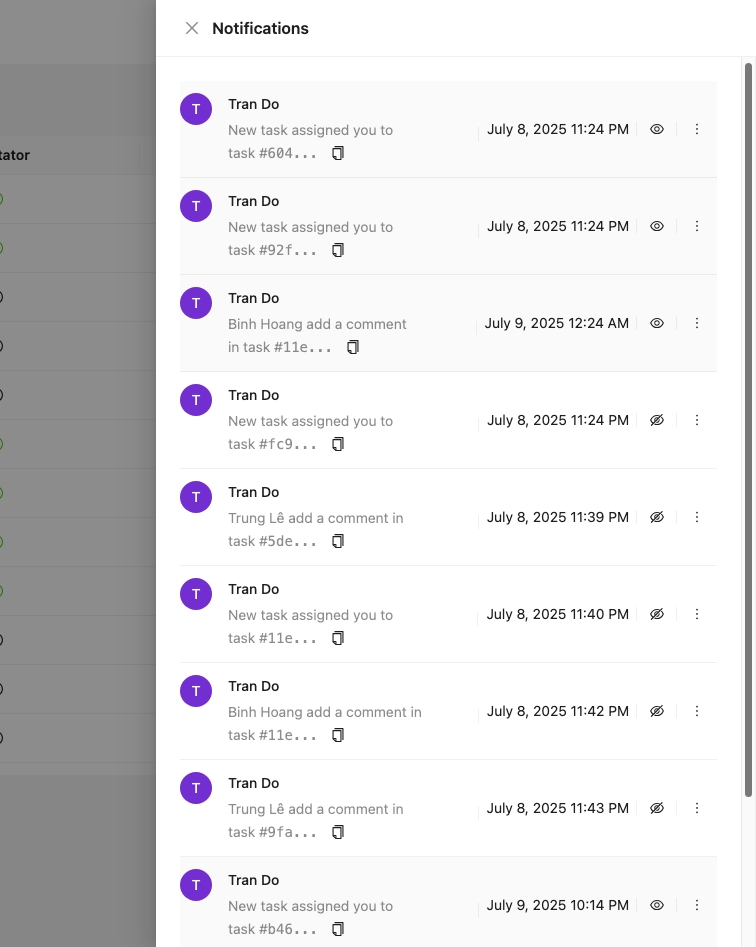
\includegraphics[width=0.6\textwidth]{content//resources//features//notifications.png}
    \caption{User Notification Panel}
    \label{fig:notifications}
\end{figure}

\subsubsection{View Tracking}
The system tracks notification viewing status, ensuring users do not miss critical updates and facilitating effective communication within the platform.

\subsection{System Integrations}
The platform is designed with extensibility in mind, allowing for seamless integration with external systems and machine learning models.

\subsubsection{Machine Learning Model Integration}
The system can connect to external ML models by storing their API endpoints. This capability enables advanced features such as model-assisted labeling (MITL), enhancing annotation efficiency and accuracy.

\section{Demo Plan}
\subsection{Metadata Auto Extraction with Q\&A Pairs Generation}
\begin{itemize}
    \item \textbf{Step 1: Input}
    \begin{itemize}
        \item \textbf{Action:} Input a full description of SeLab into the input box, along with the exact position.
        \item \textbf{Expected Result:} No immediate output is generated.
    \end{itemize}
    
    \item \textbf{Step 2: Q\&A Pair Generation}
    \begin{itemize}
        \item \textbf{Action:} Click the \emph{Generate} button.
        \item \textbf{Expected Result:} The app displays a generating process (from 0--100\%). Once complete, a new screen presents the generated Q\&A pairs.
    \end{itemize}
    
    \item \textbf{Step 3: Regeneration}
    \begin{itemize}
        \item \textbf{Action:} Click the \emph{Regenerate} button.
        \item \textbf{Expected Result:} The app displays the generating process again. A new screen shows a slightly different set of Q\&A pairs when finished.
    \end{itemize}
    
    \item \textbf{Step 4: Submission}
    \begin{itemize}
        \item \textbf{Action:} Click the \emph{Submit} button.
        \item \textbf{Expected Result:} The app shows the submission process (from 0--100\%), and upon completion, notifies the user that the metadata has been successfully updated to the remote database.
    \end{itemize}
\end{itemize}

\subsection{Indoor Space -- Floor 7th and 8th}
\begin{itemize}
    \item \textbf{Step 1: Initiate AR Session}
    \begin{itemize}
        \item \textbf{Action:} Scan the QR code located on the 8th floor.
        \item \textbf{Expected Result:} The system automatically launches the AR camera session.
    \end{itemize}
    
    \item \textbf{Step 2: Location Tracking}
    \begin{itemize}
        \item \textbf{Action:} Walk between the 7th and 8th floors and move the camera into unknown locations.
        \item \textbf{Expected Result:} The system updates and notifies the current location as the user moves between floors and warns when entering undetected environments.
    \end{itemize}
    
    \item \textbf{Step 3: Activate AI Assistance}
    \begin{itemize}
        \item \textbf{Action:} Greet the AI assistant.
        \item \textbf{Expected Result:} The AI assistant responds with guidance on how to query for a destination.
    \end{itemize}
    
    \item \textbf{Step 4: Query to I77}
    \begin{itemize}
        \item \textbf{Action:} Query “Find the path to the I77 room.”
        \item \textbf{Expected Result:} The system displays a clear navigation path leading to the I77 room.
    \end{itemize}
    
    \item \textbf{Step 5: Follow the Navigation Path}
    \begin{itemize}
        \item \textbf{Action:} Walk following the on-screen arrows.
        \item \textbf{Expected Result:} Upon arrival at the I77 room, the system notifies the user that they have reached the destination.
    \end{itemize}
    
    \item \textbf{Step 6: Query for the Research Room}
    \begin{itemize}
        \item \textbf{Action:} Query “How do I get to the research room?”
        \item \textbf{Expected Result:} The system responds with an ambiguity alert, indicating that multiple rooms could match the query (e.g., I87 and I77) and requests more information.
    \end{itemize}
    
    \item \textbf{Step 7: Clarify Destination for Software Engineering}
    \begin{itemize}
        \item \textbf{Action:} Query more specifically “Show path to the room for researching about Software Engineering.”
        \item \textbf{Expected Result:} The system displays the navigation path to the I87 room.
    \end{itemize}
    
    \item \textbf{Step 8: Query for a Room on Floor 8}
    \begin{itemize}
        \item \textbf{Action:} Query “Find the path to the room on floor 8.”
        \item \textbf{Expected Result:} The system again flags the query as ambiguous, indicating that multiple rooms could match the query (e.g., I87 and the restroom on floor 8) and requests more information..
    \end{itemize}
    
    \item \textbf{Step 9: Specify Research Room on Floor 8}
    \begin{itemize}
        \item \textbf{Action:} Combine the vague details by querying “Show me the path to the room for research on floor 8.”
        \item \textbf{Expected Result:} The system correctly displays the navigation path to the I87 room.
    \end{itemize}
\end{itemize}

\subsection{Semi-outdoor Space -- Front Campus of HCMUS}
\begin{itemize}
    \item \textbf{Step 1: Initiate AR Session}
    \begin{itemize}
        \item \textbf{Action:} Scan the QR code at the front gate.
        \item \textbf{Expected Result:} The AR camera session is activated, launching the AR interface in the semi-outdoor environment.
    \end{itemize}
    
    \item \textbf{Step 2: Verify AR Tracking}
    \begin{itemize}
        \item \textbf{Action:} Pan and move the camera around the area.
        \item \textbf{Expected Result:} The system confirms continuous tracking and reliable environment detection.
    \end{itemize}
    
    \item \textbf{Step 3: Query for the Ground Elevator}
    \begin{itemize}
        \item \textbf{Action:} Query “Find the path to the ground elevator of building I.”
        \item \textbf{Expected Result:} The system displays a clear navigation path leading to the ground elevator.
    \end{itemize}
    
    \item \textbf{Step 4: Follow the Navigation Path}
    \begin{itemize}
        \item \textbf{Action:} Walk following the on-screen arrows.
        \item \textbf{Expected Result:} The user arrives at the ground elevator of building I.
    \end{itemize}
    
    \item \textbf{Step 5: Query for the Parking Lot}
    \begin{itemize}
        \item \textbf{Action:} Query “Find the path to the parking lot.”
        \item \textbf{Expected Result:} The system flags the query as ambiguous due to multiple parking lots, requesting additional clarification.
    \end{itemize}
    
    \item \textbf{Step 6: Specify the Underground Parking Lot}
    \begin{itemize}
        \item \textbf{Action:} Query “Show me the path to the underground parking lot.”
        \item \textbf{Expected Result:} The system displays a clear navigation route to the underground parking lot.
    \end{itemize}
\end{itemize}

\chapter{Conclusion and Future Work}
\label{sec:Conclusion and Future Work}
\begin{ChapAbstract}

Chapter 5 concludes by synthesizing the thesis's contributions. The thesis introduced an AI-assisted smart navigation system combining augmented reality with advanced indoor modeling and natural language processing. The work demonstrated how integrating refined path computation with LLM-powered query interpretation enhances user navigation experiences. Future directions include automating the 3D scanning process, incorporating BLE beacons for improved tracking accuracy, and optimizing LLM query efficiency to refine further and scale the system.

\end{ChapAbstract}

\section{Summary}
This thesis presented an innovative AI-assisted intelligent navigation system that integrates augmented reality (AR) with advanced indoor environment modeling and large language models (LLMs) to overcome the limitations of traditional navigation methods. By employing mobile scanning via the Vuforia Creator application, accurate 3D models were generated and imported as Area Targets, thereby establishing a robust foundation for real-time environment tracking and localization.

A key contribution of this work is the integration of multiple components into a cohesive system that enhances the overall user experience. This includes the seamless combination of a refined NavMesh for precise path computation with an AI assistant powered by a large language model. This integration enables the system to interpret natural language queries and efficiently map them to a structured hierarchical destination database, thereby streamlining destination identification and delivering context-aware, personalized navigation support.

Overall, the thesis demonstrates the technical feasibility and practical benefits of merging AR with AI-driven natural language processing for indoor navigation. The proposed system lays the groundwork for scalable, intuitive navigation solutions that can be further refined and extended in future research.

\section{Future Work}
\label{sec:future_work}

This section outlines potential avenues for future development and research to further enhance the capabilities and robustness of the data annotation platform. These directions aim to expand functionality, improve user experience, optimize performance, and integrate advanced technologies.

\subsection{Advanced Workflow Capabilities}
The existing workflow engine provides a flexible foundation, but several enhancements can extend its power and adaptability:
\begin{itemize}
    \item \textbf{Support for More Stage Nodes}: Introducing a wider array of predefined and customizable stage types beyond current annotations, reviews, and consensus. This could include specialized nodes for data preprocessing, automated quality checks, model inference triggers, or complex data transformations, enabling even more diverse and automated pipelines.
    \item \textbf{Workflow Versioning and Rollback}: Implementing a system to version workflows would allow users to track changes, revert to previous configurations, and ensure reproducibility of annotation processes.
    \item \textbf{Complex Stage Types}: Developing more sophisticated custom stage types that incorporate complex conditional logic or external API calls.
    \item \textbf{Workflow Templates and Sharing}: Allowing users to create, save, and share workflow templates would accelerate project setup and promote best practices across different teams or organizations.
\end{itemize}

\subsection{Enhanced Annotation Tools and AI Integration}
Building upon the current annotation capabilities, future work can focus on more intelligent and efficient labeling, particularly for complex medical data:
\begin{itemize}
    \item \textbf{Customizable Annotation Interfaces}: Creating an abstraction layer or framework that allows for seamless integration with external web-based UI tools or even desktop applications like 3D Slicer. This would enable users to utilize specialized, domain-specific annotation environments while keeping project and task management centralized on the platform.
    \item \textbf{Active Learning Integration}: Implementing active learning loops where the platform identifies ambiguous data points and prioritizes them for human annotation, thereby optimizing the labeling effort and improving model performance with fewer annotations.
    \item \textbf{More AI-Assisted Labeling Tools}: Expanding the suite of AI-assisted tools to include functionalities like object tracking across frames in video annotation, semi-supervised segmentation, or generative AI-based suggestion tools.
\end{itemize}

\subsection{Improved Data Management and Caching}
Further development in data management and caching can provide deeper insights, better control, and significant performance gains:
\begin{itemize}
    \item \textbf{Advanced Reporting and Analytics}: Developing more comprehensive dashboards and reporting tools to visualize annotation progress, inter-annotator agreement (IAA), annotator performance metrics, and bottlenecks within workflows.
    \item \textbf{Caching DICOM Files (with Electron Migration Consideration)}: Implementing a robust caching mechanism for large DICOM files to significantly improve loading times for annotators. Given the substantial storage requirements for medical imaging data and the desire for improved local file access performance, exploring a migration to an Electron-based desktop application could be considered. This would enable direct access to more disk space and potentially local processing capabilities, overcoming browser storage limitations.
\end{itemize}

\subsection{Refined Security, Access Control, and Administration}
While robust, the authorization system can be further refined for broader enterprise use and to address specific security concerns:
\begin{itemize}
    \item \textbf{Enhanced Role-Based Access Control and Existing Issues}: While ABAC is foundational, a complementary enhancement to Role-Based Access Control (RBAC) could simplify common permission assignments. This involves refining predefined roles and ensuring that the interaction between ABAC policies and these roles is seamless and secure, addressing any edge cases or existing permission discrepancies identified during testing or deployment.
    \item \textbf{Auditing and Compliance Features}: Enhancing logging and auditing capabilities to track all user actions and system events. This is crucial for maintaining accountability and achieving compliance in regulated industries such as healthcare.
    \item \textbf{Organization-Level Management}: Introducing hierarchical organizational structures to manage multiple teams, projects, and users at an enterprise level, facilitating easier scaling and administrative oversight.
\end{itemize}

\subsection{Performance and Scalability Optimizations}
As the platform scales to handle larger datasets and more concurrent users, continuous performance optimization will be crucial:
\begin{itemize}
    \item \textbf{Optimized Database Queries}: Continuously optimizing database queries and indexing strategies to ensure efficient data retrieval and manipulation, especially for large-scale data and complex workflow operations.
    \item \textbf{Caching Mechanisms}: Implementing advanced caching strategies at various layers (database query results, application data, and client-side UI data) to reduce latency and improve overall responsiveness.
\end{itemize}

\subsection{User Experience and Testing}
Continuous refinement of the user interface and platform robustness based on user feedback and best practices in UI/UX design and software quality assurance:
\begin{itemize}
    \item \textbf{Intuitive Onboarding Flows (using Tour/Guides)}: Developing guided onboarding experiences, possibly incorporating interactive tours or step-by-step guides, to quickly familiarize new users with the platform's core functionalities and accelerate their productivity.
    \item \textbf{Improved Testing Application}: Expanding the test suite to include a broader range of end-to-end scenarios, stress testing, and performance benchmarks. This would involve investing in more sophisticated testing frameworks and potentially automated UI testing tools to ensure the application's stability and reliability under various conditions.
    \item \textbf{Customizable Dashboards}: Allowing users to personalize their dashboards to prioritize relevant tasks, projects, and notifications.
    \item \textbf{Mobile and Tablet Optimization}: Ensuring the platform offers a seamless and responsive experience across various devices.
\end{itemize}

By pursuing these areas, the data annotation platform can evolve into an even more comprehensive, efficient, and intelligent solution for diverse annotation needs, particularly in complex domains like medical imaging.

\import{content}{mainchaps.tex}

\nocite{D2L}
%%%%%%%%%%%%%%%%%%%%%%%%%%%%%%%%%%%%%%%%%%%%%%%%%%%%%%%
% The bibliography. Turn on page numbering.
%%%%%%%%%%%%%%%%%%%%%%%%%%%%%%%%%%%%%%%%%%%%%%%%%%%%%%%
\addtocontents{toc}{\protect\cftpagenumberson{chap}}
%%%% Soooo if IPS says there should be 5cm top margin
%%%% on the ``References'' heading page, uncomment the
%%%% line just before and after \bibliography. Repeat for
%%%% \bibliographyown if necessary
%% Increase spacing before chapter heading
\titlespacing*{\chapter}{0pt}{\dimexpr2.5cm-50pt}{\baselineskip}
\bibliography{references/refs}
% \bibliographystyle{plain}
% now change it back to normal
\titlespacing*{\chapter}{0pt}{-50pt}{\baselineskip}

%%%%%%%%%%%%%%%%%%%%%%%%%%%%%%%%%%%%%%%%%%%%%%%%%%%%%%%
% The appendices.
% If you don't have any, you may delete everything below,
% until and including \input{appendices}.
%%%%%%%%%%%%%%%%%%%%%%%%%%%%%%%%%%%%%%%%%%%%%%%%%%%%%%%


%\appendix

%\assignpagestyle{\chapter}{empty}
% * If IPS says they don't want any page numbering in the footer,
%   add \pagestyle{empty}
% * If they don't want any page numbering in the ToC either,
%   add \addtocontents{toc}{\protect\cftpagenumbersoff{chap}}
% * If they say they don't want Appendix A, B, C... to appear
%   in the ToC either, add
%     \addtocontents{toc}{\protect\setcounter{tocdepth}{-1}}
%     \addtocontents{toc}{\texbf{List of Publications}} % (to get it to appear)
% \input{appendices}
% \assignpagestyle{\chapter}{plain}

%%%%%%%%%%%%%%%%%%%%%%%%%%%%%%%%%%%%%%%%%%%%%%%%%%%%%%%
% The list of own publications.  If you don't have one, you may
% comment out the next 4 lines.
%%%%%%%%%%%%%%%%%%%%%%%%%%%%%%%%%%%%%%%%%%%%%%%%%%%%%%%
% Uncomment/comment this line if you need the List of Publications to be bold/not bold in the ToC.



%\usepackage{comment}
%\usepackage{listings}
\end{document}
